\documentclass[a4paper,14pt]{extreport}
%\usepackage{pscyr}
\usepackage[T2A]{fontenc}
\usepackage[utf8]{inputenc}
\usepackage[english,russian]{babel}
\usepackage{comment}
\usepackage{amssymb}
\usepackage{amsmath} % мат.формулы
\usepackage{amssymb} % мат.символы
\usepackage{array} % расширенные функции для оформления таблиц
% \usepackage{natbib} % расширенные функции для оформления таблиц
%\usepackage{epsfig}

\usepackage[labelsep=period]{caption} %заменить умолчальное разделение ':' на '.' в подписях к рисункам и таблицам
\usepackage{graphicx} %разрешить включение PostScript-графики
\graphicspath{{ch1_figures/}{ch2_figures/}{ch3_figures/}{ch4_figures/}{sign/}}

\usepackage{geometry} % Меняем поля страницы
\geometry{left=25mm}% левое поле
\geometry{right=10mm}% правое поле
\geometry{top=20mm}% верхнее поле
\geometry{bottom=20mm}% нижнее поле

%\bibliographystyle{mygost}
%\bibliographystyle{gost71u-utf8}
%\bibliographystyle{utf8gost705u}
\bibliographystyle{ugost2008}
%\bibliographystyle{utf8gost780u.bst}
%\bibliographystyle{ugost2003.bst}

\makeatletter
\renewcommand{\@biblabel}[1]{#1.}
%\providecommand*{\BibDash}{}
\makeatother

% % Меняем везде перечисления на цифра.цифра
% \renewcommand{\theenumi}{\arabic{enumi}} 
% \renewcommand{\labelenumi}{\arabic{enumi}}
% \renewcommand{\theenumii}{\arabic{enumii}}
% \renewcommand{\labelenumii}{\arabic{enumi}.\arabic{enumii}.}
% \renewcommand{\theenumiii}{\arabic{enumiii}}
% \renewcommand{\labelenumiii}{\arabic{enumi}.\arabic{enumii}.\arabic{enumiii}.}

\righthyphenmin=2 % Минимальное число символов при переносе - 2.

\usepackage{fancyhdr} % пакет для установки колонтитулов
\pagestyle{fancy} % смена стиля оформления страниц
\fancyhf{} % очистка текущих значений
\fancyhead[CH]{\thepage} % установка верхнего колонтитула
\renewcommand{\headrulewidth}{0pt} % убрать разделительную линию
\fancyfoot{}

\frenchspacing

\usepackage{cite}
\renewcommand{\baselinestretch}{1.3} % увеличенный межстрочный интервал
\usepackage{indentfirst} %отступ в начале параграфа
\parindent=6ex % базацный отсутп
% \usepackage{showkeys} %подписи к меткам


\renewcommand{\topfraction}{0.9}
\usepackage[pdfborder={0 0 0}]{hyperref}

\usepackage{titlesec}
\titleformat{\chapter}[block]{\Large\bfseries\centering}{Глава \thechapter.}{1ex}{}
\titleformat{\section}[block]{\normalsize\bfseries\centering}{\thesection.}{1ex}{}

%-----------------------------------------------------------%

\newcommand{\tocsecindent}{\hspace{0mm}}

%\makeatletter
%\renewcommand*\l@chapter{\@dottedtocline{0}{0em}{1.3em}}
%\makeatother

%-----------------------------------------------------------%
%-----------------------------------------------------------%

\let\vaccent=\v % rename builtin command \v{} to \vaccent{}
\renewcommand{\v}[1]{\mathbf{#1}} % for vectors
\newcommand{\gv}[1]{\ensuremath{\mbox{\boldmath$ #1 $}}} 
% for vectors of Greek letters
\newcommand{\uv}[1]{\ensuremath{\mathbf{\hat{#1}}}} % for unit vector
\newcommand{\abs}[1]{\left| #1 \right|} % for absolute value
\newcommand{\avg}[1]{\left< #1 \right>} % for average
\let\underdot=\d % rename builtin command \d{} to \underdot{}
\renewcommand{\d}[2]{\frac{d #1}{d #2}} % for derivatives
\newcommand{\dd}[2]{\frac{d^2 #1}{d #2^2}} % for double derivatives
\newcommand{\pd}[2]{\frac{\partial #1}{\partial #2}} 
\newcommand{\pdone}[2]{\partial #1 / \partial #2} 
% for partial derivatives
\newcommand{\pdd}[2]{\frac{\partial^2 #1}{\partial #2^2}} 
% for double partial derivatives
\newcommand{\pdc}[3]{\left( \frac{\partial #1}{\partial #2}
 \right)_{#3}} % for thermodynamic partial derivatives
\newcommand{\ket}[1]{\left| #1 \right>} % for Dirac bras
\newcommand{\bra}[1]{\left< #1 \right|} % for Dirac kets
\newcommand{\braket}[2]{\left< #1 \vphantom{#2} \right|
 \left. #2 \vphantom{#1} \right>} % for Dirac brackets
\newcommand{\matrixel}[3]{\left< #1 \vphantom{#2#3} \right|
 #2 \left| #3 \vphantom{#1#2} \right>} % for Dirac matrix elements
\newcommand{\grad}[1]{\nabla #1} % for gradient
\let\divsymb=\div % rename builtin command \div to \divsymb
%\renewcommand{\div}[1]{\nabla \cdot #1} % for divergence
%\newcommand{\curl}[1]{\nabla \times #1} % for curl
\let\baraccent=\= % rename builtin command \= to \baraccent
\renewcommand{\=}[1]{\stackrel{#1}{=}} % for putting numbers above =
\renewcommand{\phi}{\varphi}
\def\No{\textnumero}

\def\v{\mathbf{v}}
\def\u{\mathbf{u}}
\def\x{\mathbf{x}}
\def\n{\mathbf{n}}
\def\V{\mathbf{V}}
\def\U{\mathbf{U}}
\def\F{\mathbf{F}}
\def\n{\mathbf{n}}
\def\c{\mathbf{c}}
\def\p{\mathbf{p}}
\def\d{\partial}
\def\om{\ensuremath{\mbox{\boldmath$\omega$}}} 
\def\Om{\ensuremath{\mbox{\boldmath$\Omega$}}} 
\def\rot{\mathop{}\!\operatorname{rot}}
\def\div{\mathop{}\!\operatorname{div}}
%\def\grad{\mathop{}\!\operatorname{grad}}
\def\grad{\nabla}
%\def\Laplace{\mathop{}\!\mathbin\bigtriangleup}
\def\Laplace{\mathop{}\!\Delta}
\def\Re{\operatorname{Re}}
%\def\i{\uv{i}}

\begin{document}

\begin{titlepage}
\newpage

%\pagestyle{plain} \thispagestyle{empty}

\begin{center}
{\bf МОСКОВСКИЙ ГОСУДАРСТВЕННЫЙ УНИВЕРСИТЕТ} \\[3pt]
{\bf имени М.В. ЛОМОНОСОВА} \\[3pt]
\begin{tabular}{p{\textwidth}}
\hline {} \\[-14pt]
\end{tabular}
МЕХАНИКО-МАТЕМАТИЧЕСКИЙ ФАКУЛЬТЕТ \\[40pt]
\end{center}

\begin{flushright}
{\it На правах рукописи}\\
УДК 532.517.3: 532.542.3\\[50pt]
\end{flushright}

\begin{center}
{\bf Пиманов Владимир Олегович} \\[30pt]
{\bf ЧИСЛЕННОЕ ИССЛЕДОВАНИЕ ЛОКАЛИЗОВАННЫХ} \\ 
{\bf ТУРБУЛЕНТНЫХ СТРУКТУР В ТРУБАХ} \\[30pt]
{\it 01.02.05 -- механика жидкости, газа и плазмы} \\[30pt]
Диссертация на соискание ученой степени \\
кандидата физико-математических наук \\[30mm]
\hfill\parbox[t]{80mm}{Научный руководитель: \\ д.ф.-м.н., проф. Н.В.~Никитин} \\[5cm]
Москва -- 2017
\end{center}

\end{titlepage}


\setcounter{page}{2}
\tableofcontents

{\renewcommand \thechapter {i}
\addcontentsline{toc}{chapter}{Введение}
\thispagestyle{empty}
\phantom{.}
\chapter*{Введение}


Изучение закономерностей движения жидкостей и газов в трубах имеет большое значение как с практической, так и с теоретической точки зрения. Известно, что при небольших скоростях течения жидкость в трубах движется ламинарным образом. Такое движение хорошо организовано --- жидкие частицы могут быть объединены в слои, смещающиеся друг относительно друга без перемешивания. При достаточно больших скоростях течения, ламинарный режим сменяется турбулентным, характеризующимся наличием беспорядочных пульсаций скорости, давления, и других характеристик. Кроме того, при переходе к турбулентности многие свойства потока, такие как величина трение на стенке или форма среднего профиля скорости, качественно меняются. Как было установлено Осборном Рейнольдсом в работе 1883 года \cite{Reynolds1883}, характер течение определяет безразмерная комбинация параметров, называемая ныне числом Рейнольдса. Если число Рейнольдса $Re=UR/\nu$, вычисленное по максимальной скорости течения $U$, радиусу трубы $R$ и кинематической вязкости $\nu$, ниже критического значения, близкого к $2000$, жидкость движется ламинарным образом. При б\'{о}льших $\Re$ движение, как правило, оказывается турбулентным.

Уже Рейнольдсом было замечено, что турбулентность первоначально проявляется перемежающимся образом, когда участки возмущенного и спокойного движения следуют вдоль трубы друг за другом, практически не меняя своей протяженности. На тот момент причина пространственной локализации турбулентности установлена не была. Подробное экспериментальное исследование локализованных турбулентных структур в трубах было выполнено в \cite{Wygnanski1973}. Установлено, что в разных условиях могут возникать структуры заметно разных типов. Структуры первого типа --- турбулентные порывы ({\it turbulent puffs}) --- появляются при сильной возмущенности потока на входе в трубу в диапазоне $2000<\Re<2700$. Порывы сносятся вниз по потоку со скоростью, близкой к средней скорости течения, практически не меняя свою протяженность. Для порыва характерны размытость передней границы, на которой скорость на оси трубы плавно уменьшается от ламинарного значения на 30 -- 40\%, и резкость задней границы, на которой происходит возвращение к ламинарному течению. В последующей работе \cite{Wygnanski1975} установлено, что при $\Re<2100$ турбулентные порывы подвержены спонтанному исчезновению, а при $\Re>2300$ возможно деление порыва на два следующих друг за другом. Введено понятие {\it равновесного порыва}, характеристики которого не меняются по мере его продвижения вдоль трубы. Согласно \cite{Wygnanski1975} это наблюдается при $2100 < \Re < 2300$. 

Локализованные турбулентные структуры другого типа --- турбулентные пробки ({\it turbulent slugs}) появляются при б\'{о}льших числах Рейнольдса $\Re>3200$ только когда возмущенность потока на входе недостаточна для непосредственного возникновения турбулентности. Тогда возможен переход через турбулентные пробки --- локализованные образования, расширяющиеся по мере сноса вниз по течению. Продвигаясь по трубе, пробки нагоняют друг друга (передняя граница пробки перемещается быстрее задней), сливаясь в конечном итоге в единую турбулентную область.

В последние годы выполнен ряд подробных экспериментальных и численных исследований характеристик и свойств турбулентных порывов \cite{Priymak2004, Peixinho2006, Hof2006finite, Willis2007, Hof2008, Kuik2010, Avila2011}. Установлено, что турбулентный порыв является нестабильным образованием, склонным либо к исчезновению, либо к делению. С каждой из двух конкурирующих тенденций связано характерное время: среднее время жизни порыва до его исчезновения и среднее время до его разделения. Первое увеличивается с ростом $\Re$, второе уменьшается. Согласно точке зрения \cite{Avila2011}, значение $\Re^*=2040$, при котором происходит смена доминирования тенденций, является точкой статистического фазового перехода и может быть принята в качестве минимального критического числа Рейнольдса в круглой трубе. При $\Re<\Re^*$ турбулентный порыв скорее погибнет, чем успеет разделиться, так что возникновение развитого турбулентного течения невозможно. Наоборот, при $\Re>\Re^*$ порыв скорее успеет произвести потомство прежде, чем погибнет, что приводит к развитию незатухающего турбулентного движения.

Турбулентный порыв представляет собой интересный гидродинамический объект, который в некотором отношении может рассматриваться как структурная единица турбулентности. Можно сформулировать ряд вопросов, касающихся поведения порыва. До конца не понятен механизм, обуславливающий пространственную локализацию и самоподдержание порыва, неясны причины, побуждающие его к делению или затуханию, неизвестны факторы, определяющие его протяженность и скорость перемещения вдоль трубы.

В последние годы акцент в изучении механизма самоподдержания турбулентности в пристенных течениях смещается от лабораторного эксперимента в сторону эксперимента вычислительного, основанного на численном решении уравнений Навье--Стокса. Турбулентные порывы впервые были рассчитаны в \cite{Priymak2004}, где было показано, что пространственная локализация является внутренним свойством решений уравнений Навье--Стокса при переходных числах Рейнольдса, а не является следствием специальных начальных условий. Попытка объяснения механизма самоподдержания турбулентного порыва была предпринята в \cite{Shimizu2009}. В системе отсчета связанной с порывом, пульсации в осевой части трубы сносятся вниз по потоку. Их нелинейное взаимодействие порождает медленно меняющиеся полосчатые структуры, концентрирующиеся в пристенной области трубы, где относительная скорость течения отрицательна. Из-за этого полосчатые структуры отстают от порыва. В хвостовой части порыва в областях расположения полос замедления образуются интенсивные сдвиговые слои с точкой перегиба в профиле скорости, где в силу неустойчивости типа Кельвина--Гельмгольца порождаются мелкомасштабные пульсации, попадающие в приосевую область трубы и сносящиеся вниз по потоку. Так, согласно \cite{Shimizu2009}, выглядит цикл самопроизводства турбулентных пульсаций внутри порыва и цикл самоподдержания самой этой структуры.

Идеализированная схема, предложенная в \cite{Shimizu2009}, выглядит вполне правдоподобно, однако, на наш взгляд, сделанные выводы в должной мере не подкреплены фактическими данными. Реальная динамика порыва сложнее и неопределеннее. Ее изучение осложнено в первую очередь стохастичностью процесса, когда отдельные его фазы следуют друг за другом случайным образом. В этих условиях определенная ясность может быть получена из анализа более простых структур, аппроксимирующих порыв, недавно найденных в \cite{Skufca2006, Avila2013}. Это предельные решения, возникающие на сепаратрисе, разделяющей в фазовом пространстве области притяжения решений, соответствующих ламинарному и турбулентному режимам течения. Такие решения, наследуя ряд качественных характеристик турбулентного порыва, оказываются периодическими по времени в системе отсчета, перемещающейся вдоль трубы с постоянной скоростью. Мы будем называть такие структуры {\it модельными порывами}. Простота поведения позволяет провести исчерпывающее исследование свойств модельного порыва, которые, как мы полагаем, проясняют определенные детали поведения турбулентного порыва. 

Продолжение модельного порыва по числу Рейнольдса позволяет получить новые условно периодические решения уравнений Навье-Стокса (периодические в подходящей подвижной системе отчета), имеющие пространственно-локализованную структуру \cite{Avila2013}. Кроме того, в настоящее время известно достаточно большое число решений, имеющих вид трехмерной бегущей волны (периодичных вдоль потока и стационарных в подходящей подвижной системе отсчета) \cite{Kawahara2012}. Такие решения также допускаю детальное исследование и могут быть использованы для установления универсальности выделенных при исследовании модельного порыва закономерностей. 

Характерной особенностью модельного порыва является наличие вытянутых вдоль потока областей, скорость жидкости внутри которых существенно выше или ниже среднего значения --- полос повышенной и пониженной скорости. Такие полосы являются неотъемлемым элементом всех сценариев поддержания пристенной турбулентности \cite{Hamilton1995, Waleffe1997, Schoppa2002}, что дает основания полагать, что полученные при изучении модельного порыва результаты могут быть полезными для понимания динамики не только турбулентного порыва, но и более общего класса пристенных турбулентных течений. 

%Во введении к диссертации определяется 1) актуальность избранной темы, 2) степень ее разработанности, 3) цели и задачи, 4) научная новизна, 5) теоретическая и практическая значимость работы, 6) методология диссертационного исследования, 7) положения, выносимые на защиту, 8) степень достоверности и апробация результатов.

%В автореферате диссертации излагаются 1) положения, выносимые на защиту, 2) основные идеи и выводы диссертации, 3) показываются вклад автора в проведенное исследование, 4) степень новизны и практическая значимость результатов исследования, 4) содержатся сведения об организации, в которой выполнялась диссертация, об оппонентах, о научных руководителях и научных консультантах соискателя ученой степени (при наличии), 5) приводится список публикаций автора диссертации, в которых отражены основные научные результаты диссертации. 

{\bf Цель диссертационной работы} состоит в выявлении механизмов, ответственных за возникновение и поддержание турбулентных порывов. 
С этой целью поставлены и решены следующие \textbf{задачи}: 

%\begin{enumerate}
 $1.$  Проведено численное исследование модельного порыва --- условно периодического решения уравнений Навье-Стокса в геометрии течения в круглой трубе, имеющего пространственно-локализованную структуру. Воспроизводя ряд качественных особенностей турбулентного порыва, модельный порыв имеет более простое временное поведение, что позволяет выполнить его детальное исследование. 

 $2.$  Методом продолжения по параметру рассчитаны другие условно периодические решения уравнений Навье-Стокса в геометрии течения в круглой трубе, также имеющие пространственно локализованную структуру. Их анализ позволил оценить универсальность найденных при исследовании модельного порыва закономерностей. 

 $3.$  Рассчитаны и исследованы трехмерные решения уравнений Навье-Стокса в геометрии течения в круглой трубе и геометрии течения в плоском канале, имеющие вид бегущей волны. Анализ таких решений также позволил оценить универсальность найденных при изучении модельного порыва закономерностей. 
%\end{enumerate}

{\bf Метод исследования и достоверность результатов.}
В работе движение жидкости воспроизводится и исследуется численно, путем решения полных трехмерных уравнений Навье-Стокса для несжимаемой жидкости. Возможность адекватного описания турбулентных порывов численными решениями уравнений Навье-Стокса впервые показана в \cite{Priymak2004}. Применяемый нами численный метод совмещает конечно-разностную аппроксимацию второго порядка точности по пространственным переменным и полунеявный метод Рунге-Кутты третьего порядка точности интегрирования по времени \cite{Nikitin2006, Nikitin2006third} (детали в параграфе \ref{num_method}). Метод используется в лаборатории Общей аэродинамики института механики МГУ и других лабораториях в разных частях света уже более 20 лет и хорошо себя зарекомендовал. Код программы, реализующей метод, написан Н.В.\,Никитиным и отлажен в процессе решения большого числа задач. Расчеты выполнены с привлечением ресурсов суперкомпьютерного комплекса МГУ. Качество программной реализации численного метода и его адекватность целям работы подтверждают результаты моделирования турбулентного течения в трубе при переходных числах Рейнольдса, приведенные в параграфе \ref{puff_calc}. Турбулентность в расчетах принимает форму порывов, характеристики которых совпадают с представленными в литературе данными. 

Основным объектом исследования в работе выступает модельный порыв. Решение, соответствующее модельному порыву, является предельным состоянием решения, эволюционирующего на сепаратрисе, разделяющей в фазовом пространстве области притяжения решений, соответствующих ламинарному и турбулентному режимам течения. Решение на сепаратрисе неустойчиво и не может быть получено в эксперименте, но может быть найдено численно. Процедура нахождения решения на сепаратрисе приведена в параграфе \ref{edge_seq}. В согласии с \cite{Avila2013} решение на сепаратрисе выходит на условно периодический режим и имеет пространственно-локализованную структуру. Характеристики модельного порыва, полученные на нескольких расчетных сетках, согласуются друг с другом и с характеристиками, приведенными в работах \cite{Avila2013, Chantry2014}. Совпадение результатов подтверждает, что полученное численно решение аппроксимирует соответствующее ему решение уравнений Навье--Стокса и не зависит от выбора численного метода и параметров расчета. В \cite{Avila2013} применен полностью спектральный метод \cite{Meseguer2007} и спектрально-конечно-разностный метод \cite{Willis2009}. В нашей работе применен конечно-разностный метод~\cite{Nikitin2006}. В \cite{Chantry2014} модельный порыв воспроизведен спектрально-конечно-разностным методом \cite{Willis2009}, авторы также сообщают о совпадении результатов с \cite{Avila2013}. 

Оценить степень универсальности полученных при исследовании модельного порыва результатов позволяет анализ других решений уравнений Навье-Стокса, имеющих простое временное поведение. Можно надеяться, что общие для многих решений особенности движения могут иметь место в турбулентном течении. В работе реализован метод Ньютона-Крылова \cite{Viswanath2007, Dijkstra2014} для поиска условно периодических решений (см. параграф  \ref{Newton_seq}). Этот метод позволяет уточнять уже найденные решения и продолжать их по параметру. Продолжение модельного порыва по числу Рейнольдса позволило получить новые условно периодические решения уравнений Навье-Стокса, также, как и модельный порыв, имеющие пространственно-локализованную структуру (детали в параграфе \ref{contin_sec}). Сравнение результатов, полученных на нескольких расчетных сетках, с результатами \cite{Avila2013} позволяет сделать выводы о соответствии найденных численных решений решениям уравнений Навье--Стокса. Также, применение метода поиска решения на сепаратрисе и метода Ньютона-Крылова позволило найти три семейства решений в виде бегущих волн (см. параграф \ref{pipeTW_seq}, \ref{ductTW_seq}). Одно семейство решений относится к течению в круглой трубе и два --- к течению в плоском канале. Основные закономерности, выделенные при изучении модельного порыва, оказываются справедливы для всех исследованных решений, что в некоторой степени подтверждает универсальность этих закономерностей. 

{\bf Научная новизна и положения, выносимые на защиту.} На защиту выносятся следующие новые результаты, полученные в диссертации:

%\begin{enumerate}
 $1.$  Определены основные элементы механизма поддержания колебаний в модельном порыве --- условно периодическом решении уравнений Навье-Стокса с пространственно-локализованной структурой. Поле скорости решения может быть представлено в виде суперпозиции средней и пульсационной составляющих. Характерной особенностью среднего течения являются вытянутые вдоль потока полосы повышенной и пониженной скорости. Пульсации возникают в результате линейной неустойчивости среднего течения в областях между соседними полосами на фоне резкого изменения скорости вдоль угловой координаты. Нелинейное взаимодействие пульсаций приводит к формированию продольных вихрей, поддерживающих существование полос.

 $2.$  Показано, что в модельном порыве продольная неоднородность среднего течения не оказывает существенного влияния на формирование пульсаций. Их образование связано с неоднородностью в поперечной плоскости.

 $3.$  Обнаружен нелинейный механизм поддержания продольных вихрей, вызывающих полосчатое искажение в распределении продольной скорости. Существование продольных вихрей поддерживается нелинейным взаимодействием пульсаций продольной скорости и пульсаций продольной завихренности. Пульсации продольной завихренности образуются за счет сжатия и растяжения существующих в среднем течении вихревых трубок пульсациями продольной скорости, что обеспечивает необходимую для поддержания продольных вихрей согласованность фаз между этими пульсациями. 

 $4.$  Определены основные элементы механизма поддержания колебаний в ус\-лов\-но-периодических решениях уравнений Навье-Стокса с пространственно локализованной структурой, полученных продолжением по параметру решения, соответствующего модельному порыву. Также механизм поддержания колебаний определен в нескольких семействах решений, имеющих вид бегущей волны, описывающих течения в круглой трубе и в плоском канале. Во всех исследованных решениях механизм поддержания колебаний аналогичен найденному при исследовании модельного порыва, что в некоторой степени подтверждает универсальность этого механизма. 
%\end{enumerate}

%\textbf{Научная новизна.} В работе получены новые научные результаты:
%\begin{enumerate}
%\item Рассчитан модельный порыв --- условно периодическое решение уравнений Навье-Стокса в геометрии течения в круглой трубе, имеющее пространственно-локализованную структуру. Описаны его основные характеристики и внутренняя структура. 
%\item Методом продолжения по параметру рассчитаны другие условно периодические решения уравнений Навье-Стокса, также имеющие про\-странственно-локализованную структуру. Описаны их основные характеристики и внутренняя структура. 
%\item Рассчитано три семейства решений уравнений Навье-Стокса в виде бегущих волн. Одно семейство решений найдено в геометрии течения в круглой трубе и два семейства --- в геометрии течения в плоского канала. Описаны их основные характеристики и внутренняя структура. 
%\item В рассчитанных решениях определены основные элементы механизма поддержания колебаний. Во всех исследованных решениях за поддержание колебаний отвечает один механизм, что свидетельствует о его универсальности. 
%Поле скорости решений может быть представлено в виде суммы средней и пульсационной составляющих. Характерной особенностью среднего течения являются вытянутые вдоль потока полосы повышенной и пониженной скорости. Пульсации генерируются в результате линейной неустойчивости среднего течения в промежуточной области между полосами на фоне резкого изменения скорости вдоль угловой (поперечной) координаты. Существование полос поддерживают продольные вихри, перемещающие жидкость в нормальной к основному потоку плоскости.
%\item Обнаружен нелинейный механизм поддержания продольных вихрей, вызывающих полосчатое искажение в распределении продольной скорости. Существование продольных вихрей поддерживается нелинейным взаимодействием пульсаций продольной скорости и пульсаций продольной завихренности. Пульсации продольной завихренности образуются за счет сжатия и растяжения существующих в среднем течении вихревых трубок пульсациями продольной скорости, что обеспечивает необходимую для поддержания продольны вихрей согласованность фаз между этими пульсациями. 
%\end{enumerate}

{\bf Теоретическая и практическая значимость полученных результатов.}
Полосы повышенной и пониженной скорости являются неотъемлемым элементом всех сценариев поддержания колебаний в пристенных турбулентных течениях, что дает основания полагать, что полученные в работе представления о механизме поддержания колебаний в модельных течениях могут быть обобщены на этот класс течений. Понимание механизмов поддержания колебаний имеет первостепенное значения для предсказания характеристик пристенных турбулентных течений и разработки эффективных методов управления ими.

%{\bf Положения, выносимые на защиту.} Анализ рассчитанных в работе течений позволяет предложить следующий идеализированный цикл поддержания колебаний в них:
%\begin{itemize}
%\item В каждом решении поле скорости может быть представлено в виде суммы средней и пульсационной составляющих. Существенной особенностью среднего течения является наличие вытянутых вдоль потока полос повышенной и пониженной скорости. Пульсации возникают в результате линейной неустойчивости среднего течения в областях, расположенных между соседними полосами повышенной и пониженной скорости. В этих областях распределение средней продольной скорости имеет точки перегиба, если рассматривать его как функцию угловой (поперечной) координаты, что позволяет связать образование колебаний с неустойчивостью струйного течения с точками перегиба. 
%\item За поддержание полос повышенной и пониженной скорости ответственны продольные вихри, перемещающие жидкость в нормальной к основному потоку плоскости. Там, где медленная жидкость перемещается от стенки в основной поток, образуются полосы пониженной скорости. В промежуточных областях образуются полосы повышенной скорости. 
%\item Механизм поддержания продольных вихрей состоит в нелинейном взаимодействии пульсаций продольной скорости и пульсаций продольной завихренности. При этом в области расположения продольных вихрей пульсации продольной завихренности образуются в результате сжатия и растяжения существующих в потоке вихревых трубок пульсациями продольной скорости, что обеспечивает необходимую для поддержания продольных вихрей согласованность фаз между этими пульсациями. 
%\end{itemize}

{\bf Личный вклад автора.} 
Научному руководителю, Н.В. Никитину, принадлежит идея исследования, реализация численного метода для прямого интегрирования уравнений движения жидкости, а также руководство работой и ценные советы в процессе её выполнения. Автору диссертации принадлежат численные эксперименты и анализ полученных результатов, а также реализация метода поиска решения на сепаратрисе и метода Ньютона-Крылова для нахождения условно периодических решений уравнений Навье-Стокса. Основная работа по подготовке текста диссертации и иллюстративного материала также принадлежит диссертанту. 


{\bf Апробация работы и публикации.} 
Результаты диссертационной работы представлены на 22 научных конференциях: 
\begin{itemize}
\item Конференция-конкурс молодых ученых НИИ механики МГУ имени М.В. Ломоносова (2014, 2015, 2016, 2017 годы); 
\item Международная научная конференция студентов, аспирантов и молодых ученых <<Ломоносов>> (МГУ им. М.В.\,Ломоносова, Москва, 2014, 2015, 2016, 2017, 2018 годы); 
\item Конференция <<Ломоносовские чтения>> (НИИ механики, МГУ им. М.В. Ломоносова, 2014, 2016, 2017, 2018 годы); 
\item Международная конференция <<Нелинейные задачи теории гидродинамической устойчивости и турбулентность>> (Звенигород, 2014, 2016 годы); 
\item Школа-семинар <<Современные проблемы аэрогидродинамики>> (Сочи, 2014, 2016 годы);  
\item XI Всероссийский съезд по фундаментальным проблемам теоретической и прикладной механики (Казань, 2015 год) --- пленарный доклад;
\item 7th International Symposium on Bifurcations and Instabilities in Fluid Dynamics (Париж, 2015 год);
\item 15th European Turbulence Conference (Делфт, Нидерланды, 2015 год); 
\item 18th International Conference on the Methods of Aerophysical Research (Пермь, 2016 год);
\item Международная конференция <<Турбулентность, динамика атмосферы и климата>> (Москва, 2018 год).
\end{itemize}
Также результаты работы представлены на 5 научных семинарах:
\begin{itemize}
\item Семинар НИИ механики МГУ по механике сплошных сред под руководством А.Г.\,Куликовского, В.П.\,Карликова и О.Э.\,Мельника;
\item Семинар кафедры газовой и волновой динамики Мехмата МГУ имени М.В. Ломоносова под руководством Р.И.\,Нигматулина;
\item Семинар <<Суперкомпьютерные технологии в науке, образовании и промышленности>> на базе научно-образовательного центра <<Суперкомпьютерные технологии>> под руководством В.А.\,Садовничего;
\item Астрофизический семинар отдела теоретической физики ФИАН имени П.Н.\,Лебедева под руководством А.В.\,Гуревича;
\item Семинар лаборатории общей аэродинамики НИИ механики МГУ под руководством Н.В.\,Никитина.
\end{itemize}

По материалам диссертации опубликовано 22 научные работы, в том числе 3 статьи в рецензируемых научных изданиях, индексируемых в базах данных Web of Science и Scopus:
\begin{enumerate}
\item Pimanov V. O. Maintenance of Oscillations in Three-Dimensional Traveling Waves in Plane Poiseuille Flows // Moscow University Mechanics Bulletin. —
2018. — Vol. 73, Iss. 4. — Pp. 91–96. — SJR 2016: 0.108.
\item Никитин Н. В., Пиманов В. О. О поддержании колебаний в локализованных турбулентных структурах в трубах // Изв. РАН. МЖГ. — 2018. — No 1. — С. 68—76. — Перевод: Nikitin N. V., Pimanov V. O. Sustainment of Oscillations in Localized Turbulent Structures in Pipes // Fluid Dynamics. — 2018. — Vol. 53, Iss. 1. — Pp. 65–73. — Impact Factor 2017: 0.608.
\item Никитин Н. В., Пиманов В. О. Численное исследование локализованных турбулентных структур в трубах // Изв. РАН. МЖГ. — 2015. — No 5. — С. 64—75. — Перевод: Nikitin N. V., Pimanov V. O. Numerical study of localized turbulent structures in a pipe // Fluid Dynamics. — 2015. — Vol. 50, Iss. 5. — Pp. 655–664. — Impact Factor 2017: 0.608.
\end{enumerate}
Статья в журнале, входящем в перечень изданий, рекомендованных ВАК при Министерстве образования и науки РФ:
\begin{enumerate}
\item[4.] Никитин Н. В., Пиманов В. О. Локализованные турбулентные структуры в круглой трубе // Учен. зап. Казан. ун-та. Сер. Физ.-матем. науки. —
2015. — Т. 157, кн. 3. — С. 111—116. — Импакт-фактор РИНЦ 2017: 0,248.
\end{enumerate}
Три статьи в сборниках трудов:
\begin{enumerate}
\item[5.] Пиманов В. О. Некоторые детали механизма самоподдержания турбулентности в пристенных течениях // Труды конференции-конкурса молодых
ученых 10-12 октября 2016 г. / под ред. А. Г. Куликовского, В. А. Самсонова. — М. : Изд-во Моск. ун-та, 2017. — С. 46—53.
\item[6.] Пиманов В. О. О механизме самоподдержания локализованных турбулентных структур в трубах // Труды конференции-конкурса молодых ученых. 12–14 октября 2015 г. / под ред. А. Г. Куликовского, В. А. Самсонова. — М. : Изд-во Моск. ун-та, 2016. — С. 44—51.
\item[7.] Пиманов В. О. Пространственно-локализованные турбулентные структуры в круглой трубе // Труды конференции-конкурса молодых ученых. 13–17 октября 2014 г. / под ред. А. Г. Куликовского, В. А. Самсонова. — М. : Изд-во Моск. ун-та, 2016. — С. 42—50.
\end{enumerate} 
и 15 тезисов докладов.

Работа отмечена наградами:
\begin{itemize}
\item Диплом 2-ой степени конференции--конкурса молодых ученых НИИ механики МГУ 2014 года;
\item Диплом 1-ой степени за лучшую работу аспиранта и диплом 3-ей степени конференции-конкурса молодых ученых НИИ механики МГУ 2015 года;
\item Диплом 1-ой степени за лучшую работу аспиранта и диплом 3-ей степени конференции-конкурса молодых учёных НИИ механики МГУ 2016 года;
\item Вторая премия конкурса молодых научных сотрудников МГУ~им.~М.В.~Ломоносова 2015 года;
\item Грамота за лучший доклад на международной научной конференции студентов, аспирантов и молодых ученых <<Ломоносов>> 2015, 2017 и 2018 годов.
\end{itemize}

{\bf Структура и объем диссертации.} 
Диссертация состоит из титульного листа, оглавления, введения, четырех глав, заключения и списка литературы. В первой главе приведены постановка задачи и численный метод ее решения. Во второй главе описана процедура получения модельного порыва и его основные свойства. В третьей главе дано описание механизма образования продольных вихрей. Четвертая глава посвящена отличным от модельного порыва решениям уравнений Навье-Стокса, исследованным в работе. Общий объем диссертации --- 124 страницы. Список литературы содержит 92 пункта. 


%Хочу выразить благодарность своему научному руководителю, Николаю Васильевичу Никитину, за постановку интересных задач, одна из которых привела к результатам, описанным в диссертации. Также хочу поблагодарить сотрудников кафедры гидромеханики мехмата МГУ и, в первую очередь, ее заведующего, Карликова Владимира Павловича, за возможность учиться у выдающихся исследователей в области гидромеханики и настоящих профессионалов своего дела. В заключение, хочу поблагодарить свою семью и особенно свою жену Дарью за помощь и всестороннюю поддержку. 





}

\chapter{Метод решения}

\section{Введение}


Представленное в диссертационной работе исследование выполнено методом прямого численного моделирования. 


During the last decades, direct numerical simulations (DNS) have been recognized as a powerful and reliable tool for studying the basic physics of turbulence. 


\section{Математическая постановка задачи}

Рассматривается течение вязкой несжимаемой жидкости в прямой трубе круглого сечения. Жидкость считается однородной --- её плотность $\rho$ и вязкость $\mu$ во всем объеме трубы постоянны. Движение вызывается внешним градиентом давления, направленным вдоль трубы.


Поле скорости $\v(\x,t)$ удовлетворяет уравнению несжимаемости
\begin{equation} \label{eq0}
\nabla \cdot \v = 0.
\end{equation}

Движение жидкости описывается уравнениями Навье-Стокса, которые для несжимаемой жидкости имеют вид
\begin{equation} \label{NSeq_dynamic}
\pd{\v}{t} = - (\v, \nabla) \v - \frac{1}{\rho}\nabla \Pi + \frac{\mu}{\rho} \nabla^2 \v.
\end{equation}
Здесь $\Pi = \Pi(\x,t)$ --- поле давления. Уравнения решаются в цилиндрической системе координат $(x,r,\theta)$, где $x$ --- продольное, $r$ --- радиальное и $\theta$ --- угловое направления, $t$ --- время. 


На твердой стенке трубы радиуса $R$ ставятся условия прилипания
\begin{equation} \label{bc0}
\v = 0 \text{ при } r = R.
\end{equation}
В направлении движения устанавливаются условие периодичности с периодом $L_x$. Давление $\Pi$, непосредственно, периодическим не является. Оно представляется в виде суммы периодической $p$ и линейной вдоль трубы $Dx$ составляющих. Подстановка $\Pi = p + Dx$ в \eqref{NSeq_dynamic} дает уравнение
\begin{equation} \label{NSeq_periodic}
\pd{\v}{t} = - (\v, \nabla) \v - \frac{D}{\rho}\i - \frac{1}{\rho}\nabla p + \frac{\mu}{\rho} \nabla^2 \v.
\end{equation}
Здесь $\i$ -- единичный орт, направленный вдоль трубы. В уравнении \eqref{NSeq_periodic} все переменные удовлетворяют условию периодичности вдоль трубы
\begin{equation} \label{bc1}
[\v, p](x,r,\theta,t) = [\v, p](x+L_x,r,\theta,t).
\end{equation}

Величина $D$ представляет собой внешний градиент давления, которые определяется из условия постоянства расхода жидкости, протекающей через трубу. Постановка задачи может быть легко обобщена на случай наличия внешних потенциальных сил $\F = \nabla U$. За $D$ в этом случае следует обозначить разность внешнего градиента давления и средней вдоль трубы составляющей $F_x$. Не вошедшая в $D$ часть $\F$ потенциальна. Разность периодической вдоль трубы части давления и её потенциала составляет $p$. 

Поставленная задача, определяемая уравнениями \eqref{eq0}, \eqref{bc0}, \eqref{NSeq_periodic}, \eqref{bc1}, имеет единственное решение для каждого начального поля скорости $\v_0(\x)$, удовлетворяющего условию несжимаемости \eqref{eq0}. Известно аналитическое решение задачи, называемое течением Пуазейля, соответствующее ламинарному режиму течения. Оно существует при всех значениях параметров и задается формулой
\begin{equation}
\v = (U (1 - (r / R)^2), 0, 0).
\end{equation}
Здесь величина $U = - D R^2\mu^{-1}/4 $ определяется по градиенту давления $D$ и соответствует максимальной скорости в ламинарном течении, которую оно достигает на оси трубы. Несложно показать, что средняя скорость течения $U_q$, вычисленная как отношение расхода к площади сечения трубы, в этом случае равна $U/2$. 


В работе все вычисления выполняются в безразмерных переменных. В качестве масштабов выступают радиус трубы $R$, максимальная скорость в ламинарном течении $U$ и плотность жидкости $\rho$. Переход к безразмерным единицам измерения, обозначенным штрихами, выполняется по формулам
\begin{equation} \label{dim_less_eqs}
R x' = x,  R r' = r, RU^{-1} t' = t, U\v' = \v , \rho U^2 p' = p, \rho U^2 R^{-1} D' = D, R L'_x = L_x.
\end{equation}

В безразмерных единицах измерения уравнения \eqref{eq0}, \eqref{bc0}, \eqref{NSeq_periodic}, \eqref{bc1} принимают вид (штрихи опущены):
\begin{equation}\label{eq0_Re}
\nabla \cdot \v = 0,
\end{equation}
\begin{equation}\label{NSeq_Re}
\pd{\v}{t} = - (\v, \nabla) \v - \i D - \nabla p + \frac{1}{\Re} \nabla^2 \v,
\end{equation}
\begin{equation}\label{bc0_Re}
\v = 0 \text{ при } r = 1,
\end{equation}
\begin{equation}\label{bc1_Re}
[\v, p](x,r,\theta,t) = [\v, p](x+L_x,r,\theta,t)
\end{equation}
Здесь $\Re = \rho R U / \mu$ --- число Рейнольдса, один из двух параметров системы. Вторым параметром является $L_x$. Величина $D$ подбирается из условия постоянства расхода так, что $U_q = 1/2$ в безразмерных единицах. В случае ламинарного течения она выражается в явном виде: $D = - 4 \Re^{-1}$. Ламинарное течение в безразмерном виде задается более простым выражением 
\begin{equation}
\v = (1 - r^2, 0, 0).
\end{equation}

Многие авторы вводят число Рейнольдса иначе, через расходную скорость $U_q$ и диаметр трубы $D$. Несложно показать, что значение числа Рейнольдса, введенного таким образом, совпадает со значением числа Рейнольдса, введенного выше. Однако, например, единица измерения времени $DU_q^{-1}$ в этом случае увеличивается в 4 раза.

В процессе решения задачи возникает необходимость перехода в подвижную систему координат. Выполняя переход, удобно сохранить в качестве тела, относительно которого определяются скорости, стенки трубы. В этом случае граничные условия и значения скорости не зависят от системы отсчета, но в уравнении движения \eqref{NSeq_Re} возникает новое слагаемое
\begin{equation}\label{NSeq_cf}
\pd{\v}{t} = c_f \pd{\v}{x} - (\v, \nabla) \v - \i D - \nabla p + \frac{1}{\Re} \nabla^2 \v. 
\end{equation}
Возникшее слагаемое отвечает за перенос решения вдоль трубы со скоростью $-c_f$, где $c_f = c_f(t)$ --- скорость перемещения системы координат, может быть функцией времени. Уравнение неразрывности \eqref{eq0_Re} при переходе, выполненном таким образом, не меняется. 


Поставленная задача сформулирована традиционным образом для прямого расчета турбулентных потоков в прямых каналах. В такой постановке удается воспроизводить характеристики течения, устанавливающегося на большом удалении от входа в трубу, решая уравнения лишь в ограниченной расчетной области. Условие периодичности освобождает от необходимости устанавливать условия на входе и выходе из трубы. В тоже время, увеличивая длину периода $L_x$, можно минимизировать влияние этого условия на поток. Для того, чтобы иметь возможность воспроизвести в расчете локализованные турбулентные структуры, необходимо выдирать длину $L_x$ достаточно большой, не менее $40$ диаметров трубы. 


\section{Численный метод}

\begin{comment}
Поставленная задача решается численно конечно-разностным методом \cite{nikitin2006method}. Метод формулируется относительно уравнения движения \eqref{NSeq_Re}, преобразованного к виду 
\begin{equation}\label{NSeq_om}
\pd{\v}{t} = - \i D + \v \times \om - \nabla P - \frac{1}{\Re} \rot \om
\end{equation}
Здесь $\om = \rot \v$ --- вектор завихренности, посчитанный по полю скорости $\v$, $P = p + |\v|^2/2$ --- полное кинематическое давление. Эквивалентность уравнений \eqref{NSeq_Re} и \eqref{NSeq_om} следует из векторных тождеств
\begin{equation*}
-(\v, \nabla) \v = \v \times \rot \v - \nabla |\v|^2/2,
\end{equation*}
\begin{equation*}
\nabla^2 \v = \grad \div \v - \rot \rot \v.
\end{equation*}
\end{comment}

Поставленная задача решается численно конечно-разностным методом \cite{nikitin2006method}, в цилиндрической системе координат $(x,r,\theta)$. Расчетная область в переменных $(x,r,\theta)$ имеет форму параллелепипеда
\begin{equation}
0 < x < L_x, 0 < r < 1, 0 < \theta < 2\pi.
\end{equation}
При решении уравнений в этих переменных необходимо дополнительно установить условия периодичности в направлении $\theta$ и ограниченности решения при $r=0$.

В переменных $(x,r,\theta)$ в расчетной области вводится прямоугольная система координат, однородная в направлениях $x$ и $\theta$. В радиальном направлении вводится растяжение сетки, что позволяет сгустить её вблизи стенки. Во всех расчетах, приведенных ниже, параметр растяжения выбран так, что размер ячейки в радиальном направлении около стенки в 4 раза меньше, чем в центре трубы. 

При дискретизации уравнений применен подход, при котором различные неизвестные определяются в различных точках сетки. Так, давление $p$ относится к центру ячеек. Компоненты вектора скорости $v_k$ относятся к центрам граней, нормальных к направлению $k$. В процессе счета и при анализе решений возникает необходимость вычисления завихренности $\omega$. Компоненты вектора завихренности $\omega_k$ относятся к центрам ребер, параллельных направлению $k$. При таком подходе говорят, что неизвестные определены на смещенных или разнесенных сетках. Он позволяет естественным образом ввести аппроксимацию уравнения второго порядка точности по пространству. 

Пространственная дискретизация введена таким образом, что сохраняется ряд важных консервативных свойств исходной системы. В частности, тождественно равна нулю дивергенция вязких слагаемых в \eqref{NSeq_Re}, что гарантирует, что это слагаемое не производит массы. Также тождественно равна нулю завихренность градиента давления, что обеспечивает отсутствие влияния давления на эволюцию завихренности непосредственно. 

При моделировании турбулентных течений важно аккуратно воспроизводить изменение кинетической энергии системы. Уравнение, описывающее его, возникает в результате скалярного умножения на $\v$ уравнений движения \eqref{NSeq_Re} с последующим суммированием по всей расчетной области. Важным свойством системы является то, что в уравнении Навье-Стокса для несжимаемой жидкости градиент давления и нелинейные слагаемые не производят кинетической энергии, а лишь перераспределяют уже существующую. В конечно-разностной постановке строго выполняются тождества, выражающие этот факт, выполненные при \eqref{eq0_Re}, \eqref{bc0_Re}, \eqref{bc1_Re}
$$
\int_V \v \cdot \nabla p\ d\tau= \int_V \nabla (\v p) d\tau = \int_{\Sigma} p v_n d\sigma = 0, 
$$
$$
\int_V \v \cdot (\v, \nabla) \v\ d\tau = \int_V (\v, \nabla)\frac{|\v|^2}{2}\ d\tau = \int_V \nabla (\v \frac{|\v|^2}{2}) d\tau = \int_{\Sigma} \frac{|\v|^2}{2} v_n d\sigma = 0.
$$
Здесь $V$ --- расчетная область, $\Sigma$ --- её граница, $v_n$ --- нормальная составляющая скорости на границе. Также строго выполняется дискретный аналог уравнения изменения полной кинетической энергии $E$, записанного в следующем виде
\begin{equation} \label{Eeq}
\d{E}{t} = - \frac{1}{2}DV - \frac{1}{\Re} \int_{V} |\omega|^2 d\tau,
\end{equation}
$$
E = \frac{1}{2}\int_{V} |\v|^2 d\tau.
$$
Изменение полной энергии происходит за счет внешнего градиента давления $D$ и вязкой диссипации. 

Интегрирование по времени выполняется полу-неявным методом Рунге-Кутты третьего порядка точности \cite{Nikitin2006Third}. В силу нелинейности оператора Навье-Стокса реализовать полностью неявный метод продвижения по времени затруднительно. Однако наибольшая жесткость системы на достаточно подробных сетках вызвана вязкими слагаемыми. В силу их линейности они могут быть разрешены неявно в то время, как другие слагаемые в операторе Навье-Стокса разрешаются явно. Такой подход позволяет существенно увеличить допустимый временной шаг в сравнении с явными методами. Реализованный алгоритм допускает автоматический выбор шага интегрирования исходя из условия сохранения локальной точности получаемого решения. Таким образом шаг интегрирования автоматически адаптируется к изменением в структуре течения, и не требует явного его задания во время счета. 


На каждом шаге по времени возникает необходимость по известному полю скорости $\v$ определить давление $p$. Для этого необходимо решить уравнение Пуассона, возникающее в результате применения оператора дивергенции к уравнению движения \eqref{NSeq_Re} при условии несжимаемости \eqref{eq0_Re}, имеющее вид
\begin{equation}\label{Peq}
\nabla^2 p = \div \tilde \v,
\end{equation}
$$
\tilde \v = - (\v,\nabla)\v + \frac{1}{\Re}\nabla^2 \v. 
$$
Правая часть уравнения \eqref{Peq} известна. Давление также удовлетворяет условию периодичности в направлениях $x$ и $\theta$. На оси трубы значение давления ограничено. Условие на твердой стенке возникает в результате проектирования уравнения \eqref{NSeq_Re} на направление нормали $n$
$$
\pd{p}{n} = \tilde v_n.
$$


Простая геометрия расчетной области позволяет применять прямые методы решения возникающей линейной системы. Метод решения задачи для давления основан на применении быстрого преобразования Фурье в направлениях $x$ и $r$. В радиальном направлении система решается методом прогонки. Общая сложность решения задачи для давления составляет $O(N \log N)$, где $N$ --- количество ячеек в сетке. Решение задачи для давления составляет основную вычислительную сложность используемого метода. 

\section{Методические расчеты}


Приводимые ниже результаты расчетов в диапазоне $1670\leqslant Re\leqslant 2800$ получены при $L_x=200$ с пространственным разрешением $2048 \times 64 \times 128$ в продольном, радиальном и угловом направлении соответственно. Расчеты на более грубой сетке $1024\times32\times64$ во всех рассмотренных случаях дают результаты совпадающие качественно и близкие количественно.

Стартуя с начальных данных в виде некоторого трехмерного возмущения течения Пуазейля, уравнения Навье--Стокса интегрируются до выхода решения на тот или иной режим. Установление решения, отвечающего турбулентному течению происходит в том случае, когда амплитуда начального возмущения достаточно велика, в противном случае возмущения затухают со временем, и решение в конечном итоге возвращается к ламинарному течению Пуазейля. Турбулентный режим за пределами диапазона переходных чисел Рейнольдса $Re\geqslant3000$ имеет вид статистически стационарного процесса и не зависит от конкретного вида начальных условий, при которых он был получен. Течение при этом однородно в продольном направлении, его статистические характеристики согласуются с имеющимися экспериментальными данными. При $\Re\leqslant2600$ в распределении скорости вдоль трубы появляется неоднородность, которая при $\Re\lesssim2200$ приобретает форму двигающейся вдоль трубы цепочки из нескольких пространственно-локализованных структур, разделенных участками ламинарного течения. Конкретное число получающихся в решении турбулентных структур зависит от начальных условий. Кроме того, как было отмечено выше, это число может меняться в процессе эволюции в результате исчезновения или деления отдельных структур. Получаемые в расчетах пространственно-локализованные турбулентные структуры хорошо согласуются с наблюдаемыми в экспериментах турбулентными порывами, что позволяет нам пользоваться этим их наименованием. Отметим, что турбулентные порывы формируются и на некотором отрезке времени существуют в расчетах и при $Re<2000$, вплоть до $Re=1670$. Однако, в этом случае не только число порывов в пределах расчетной области, но и время их существования является случайной величиной и зависит от конкретных начальных условий. Представленная на фиг.~1 визуализация рассчитанных течений в диапазоне $1680\leqslant Re\leqslant2800$ демонстрирует эволюцию локализованных структур при изменении числа Рейнольдса.






\chapter{Исследование модельного порыва}


В прямых трубах круглого сечения, как и в некоторых других сдвиговых течениях, переход к турбулентности может происходить без потери ламинарным течением линейной устойчивости. В частности, в приведенной в разделе \ref{math_section} постановке ламинарное течение (течение Пуазейля в круглой трубе) линейно устойчиво при всех числах Рейнольдса \cite{Kerswell2005}. Для выхода на турбулентный режим течения необходимо внести в поток возмущения достаточно большой амплитуды, в то время как малые возмущения ламинарного течения затухают. В таких условиях существуют возмущения некоторой критической амплитуды, отделяющие возмущения, вызывающие переход к турбулентности, от затухающих. В фазовом пространстве соответствующие критическим возмущениям решения принадлежат сепаратрисе, отделяющей области притяжения решений, соответствующих ламинарному и турбулентному режимам течения. Принадлежащее в первый момент времени сепаратрисе решение остается на сепаратрисе. Хотя решение, эволюционирующее на сепаратрисе, неустойчиво и не может наблюдаться в эксперименте, оно может быть получено численно. Замечено, что решение на сепаратрисе сохраняет некоторое характерные черты турбулентного течения, но при этом имеет более простую форму и динамику. 

Метод поиска решения на сепаратрисе предложен в работе \cite{Skufca2006}. Первые расчеты решения на сепаратрисе в круглой трубе выполнены в расчетной области небольшой протяженности (с условием периодичности вдоль потока) \cite{Schneider2007}. В расчетах \cite{Mellibovsky2009transition, Duguet2010}, выполненных в протяженной расчетной области, обнаружено, что при переходных числах Рейнольдса решение на сепаратрисе в круглой трубе имеет пространственно локализованную структуру. При этом, если турбулентность существует в форме пространственно локализованных порывов до $\Re \approx 2700$, то решение на сепаратрисе имеет пространственно локализованную структуру по крайней мере до $\Re = 6000$. С ростом числа Рейнольдса амплитуда отклонения от ламинарного течения и протяженность области локализации в решении на сепаратрисе снижаются \cite{Duguet2010}, что дает основание полагать, что решение на сепаратрисе сохраняет локализованную структуру и при больших числах Рейнольдса (хотя расчеты при больших $\Re$ не проводились). Как отмечено в \cite{Duguet2010, Avila2013}, решение на сепаратрисе в круглой трубе воспроизводит ряд характерных особенностей турбулентного порыва, и при небольших значениях числа Рейнольдса их характеристики оказываются близки друг к другу. Структуры, напоминающие локализованное решение на сепаратрисе, наблюдались в экспериментах \cite{deLozar2012} и в численных расчетах \cite{Manneville2011} при затухании турбулентного течения. 
% Расчеты решения на сепаратрисе в плоском течении Куэтта \cite{Schneider2008}
% Решение на сепаратрисе в плоском течении Куэтта в протяженной расчетной области имеет локализованную структуру \cite{Duguet2009}

В работе \cite{Avila2013} обнаружено, что при наложении на решение, описывающее течение в круглой трубе, дополнительных условий симметрии при переходном значении числа Рейнольдса решение, эволюционирующее на сепаратрисе, приближается к условно периодическому решению. Предельное решение сохраняет пространственно локализованную структуру, но в сопутствующей системе отсчета оказывается периодическим по времени. Помимо пространственной локализации предельное решение воспроизводит некоторые другие характерные особенности турбулентного порыва (см. раздел \ref{edge_char_seq}). Мы будем называть это решение {\it модельным порывом}. Простота поведения модельного порыва позволяет выполнить его подробное исследование, что может помочь прояснить свойства турбулентного порыва. 

В главе представлен метод получения модельного порыва, описаны его основные характеристики и внутренняя структура; даны оценки достоверности полученных результатов. Детальное описание внутренней структуры модельного порыва выполнено автором диссертации и является новым научным результатом. Основные результаты, приведенные в этом разделе, опубликованы в работах автора диссертации \cite{MZG2015, Kazan2015, KMU2015}. 


\section{Получение модельного порыва} \label{edge_seq}

Следуя \cite{Avila2013}, решение поставленной в разделе \ref{math_section} задачи ищется с дополнительными ограничениями диаметральной симметричности и $\pi$-периодичности в угловом направлении:
\begin{equation}\label{sym_eq}
(v_x, v_r, v_\theta)(x, r, -\theta, t) = (v_x, v_r, -v_\theta)(x, r, \theta, t),
\end{equation}
\begin{equation}\label{per_eq}
(v_x, v_r, v_\theta)(x, r, \theta+\pi, t) = (v_x, v_r, v_\theta)(x, r, \theta, t).
\end{equation}
Здесь $(x, r, \theta)$ --- цилиндрические координаты, $(v_x, v_r, v_\theta)$ --- продольная, радиальная и угловая компоненты вектора скорости. Наложение ограничений \eqref{sym_eq}, \eqref{per_eq} упрощает поведение решения в пространстве, делает его более определенным. Условие \eqref{sym_eq} ограничивает возможность смещения турбулентных структур в угловом направлении.  Турбулентные порывы, рассчитанные при $Re=2000$ с учетом и без учета условий \eqref{sym_eq}, \eqref{per_eq} изображены на рисунке~\ref{3D_img} (представлены области пониженной и повышенной на $0.1$ скорости относительно течения Пуазейля). В обоих случаях порыв имеет центральное ядро с пониженной скоростью и систему вытянутых вдоль стенки трубы, чередующихся в угловом направлении полос замедления и ускорения. На симметричном порыве полосы гораздо более структурированы. Их угловое положение не меняется в процессе эволюции: угловые области $\theta=k\pi/2$, $k$ от $0$ до $3$, где в силу \eqref{sym_eq}, \eqref{per_eq} угловая компонента скорости тождественно равна нулю, заняты полосами ускорения, промежуточные области $\theta=\pi/4+k\pi/2$ --- полосами замедления. На порыве без условий симметрии наблюдаются значительные по амплитуде случайные по пространственному расположению флуктуации, разрывающие сплошность полосчатых структур. На симметричном порыве тоже заметна флуктуирующая компонента, которая в этом случае выглядит гораздо более регулярной. Отметим, что несмотря на заметную пространственную регулярность, временн\'{о}е поведение симметричного порыва остается хаотичным.


\begin{figure}[h]
\center{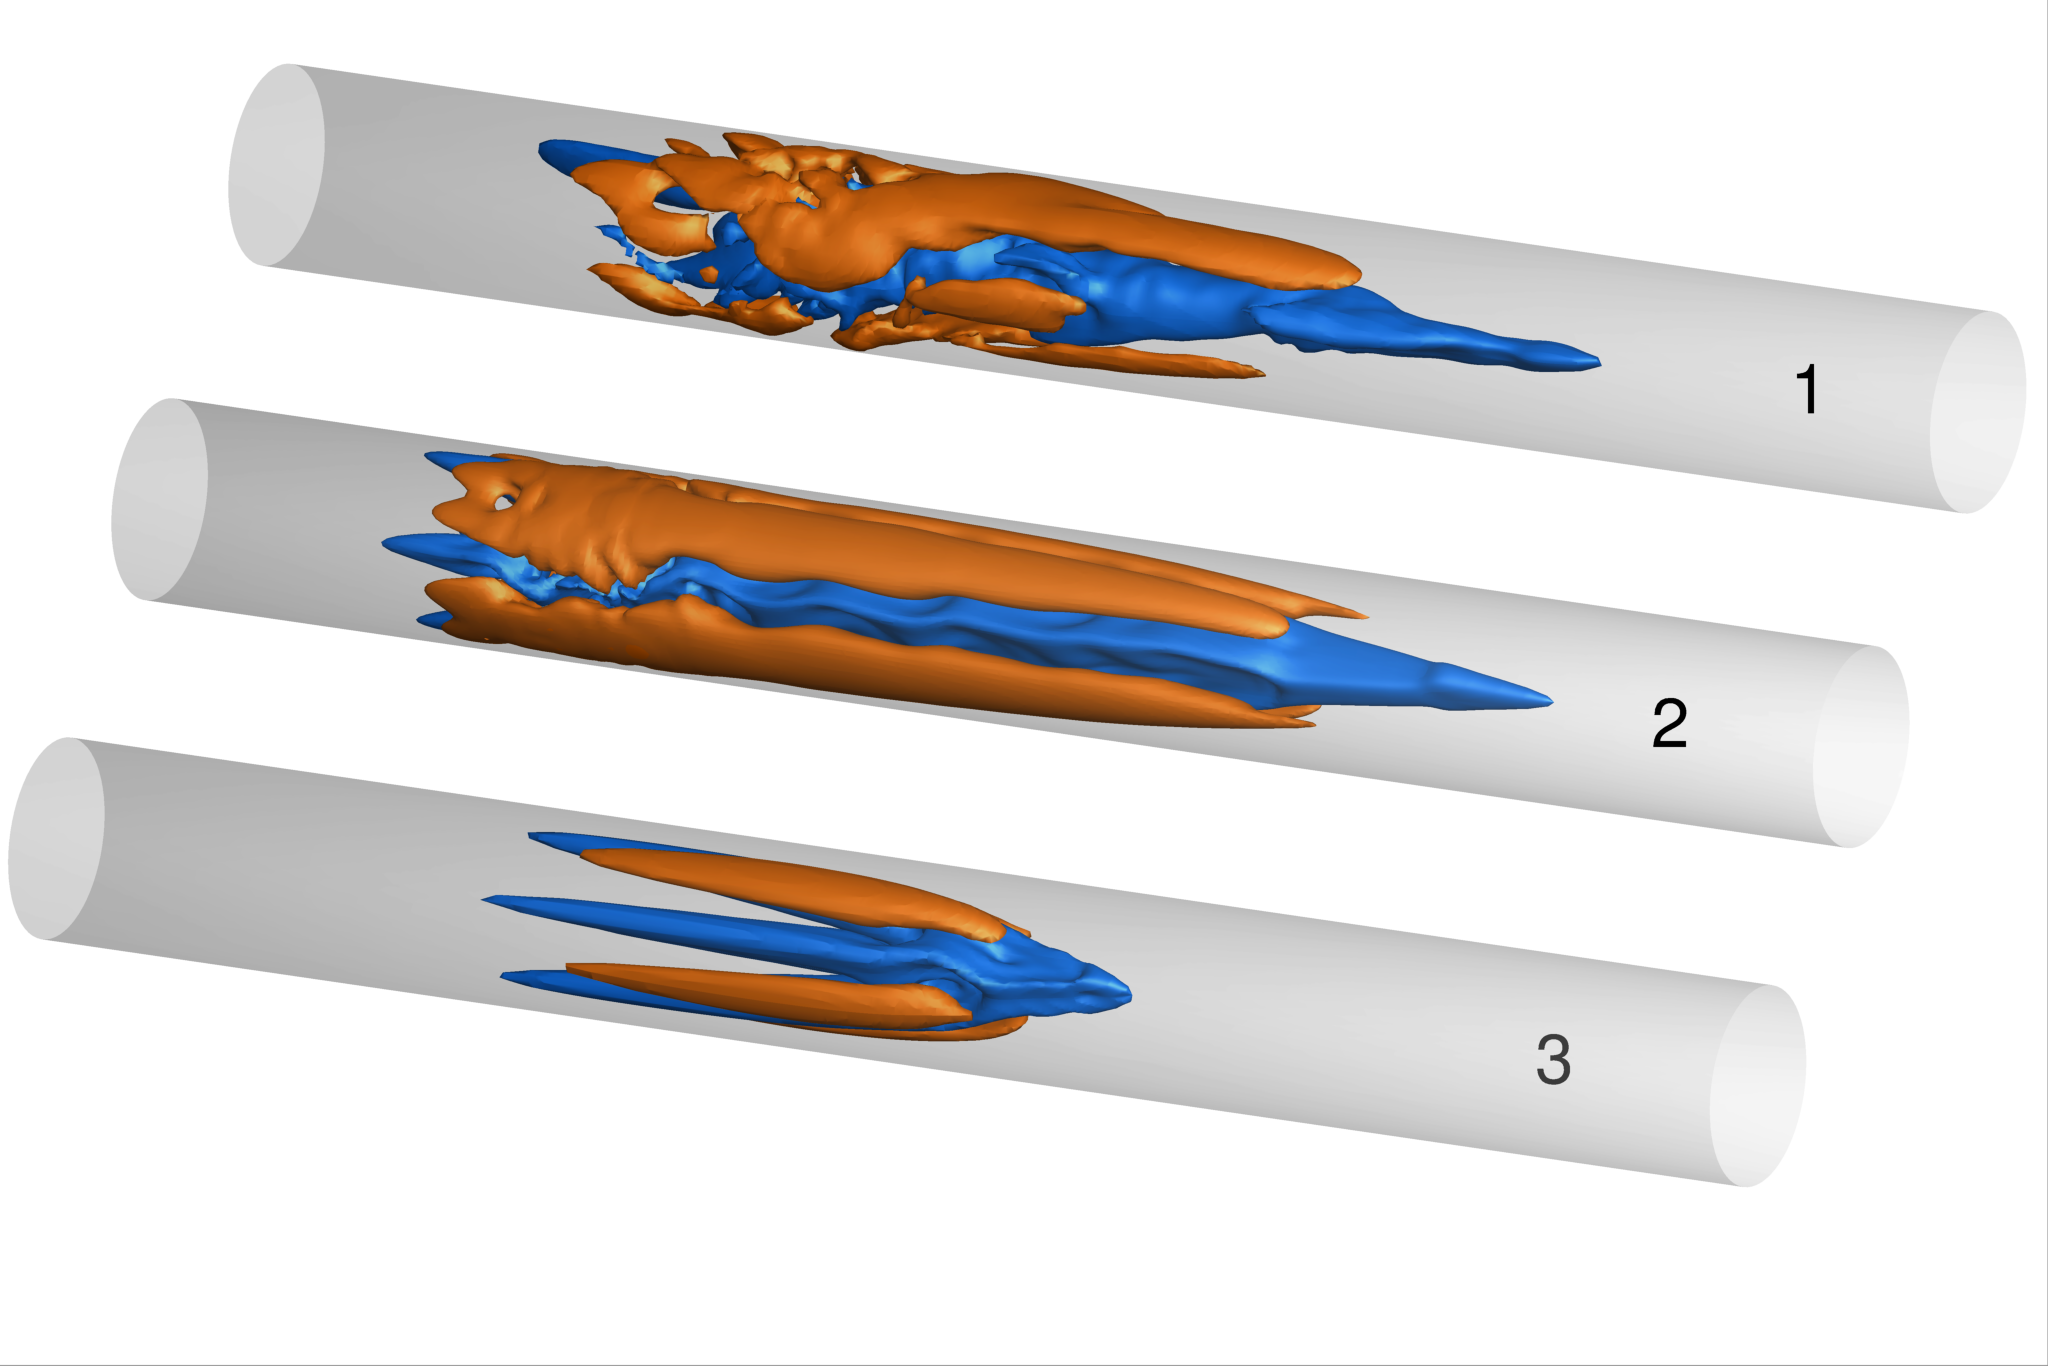
\includegraphics[width=1\linewidth]{3D_cmp.png}}
\caption{Визуализация численных расчетов турбулентных порывов: 1 --- $\Re = 2000$; 2 --- $\Re = 2000$ с учетом \eqref{sym_eq}, \eqref{per_eq}; 3 --- решение на сепаратрисе, $\Re = 2200$. Темным и светлым тоном выделены поверхности скорости $-0.1$ и $+0.1$ относительно скорости течения Пуазейля. Поток направлен слева направо.}
\label{3D_img}
\end{figure}

Предельное решение на сепаратрисе получено при $\Re=2200$. Условие \eqref{per_eq} при \eqref{sym_eq} порождает условие отражения относительно сечения $\theta = \pi/2$, аналогичное условию отражения относительно сечения $\theta = 0$:
\begin{equation} \label{sym2_eq}
(v_x, v_r, v_\theta)(x, r, \pi/2 + \theta, t) = (v_x, v_r, -v_\theta)(x, r, \pi / 2 - \theta, t).
\end{equation}
С учетом \eqref{sym_eq}, \eqref{sym2_eq} расчет проводился для четверти объема трубы $0\leqslant\theta\leqslant\pi/2$. Исходное решение найдено при $L_x = 80$ на сетке, содержащей $512 \times 32 \times  32$ ячеек в продольном, радиальном и угловом направлениях. 

Предварительно найденное турбулентное решение $\v_{turb}(\x,t)$ используется в итерационной процедуре отыскания предельного решения на сепаратрисе. Задача решается с начальным условием
\begin{equation} \label{edge_init_eq}
\v(\x,t=0) = \v_{Pois}(\x)+\alpha(\v_{turb}(\x,t=t_0) - \v_{Pois}(\x)).
\end{equation}
Здесь $\v_{Pois}=(1-r^2,0,0)$ --- течение Пуазейля, $t_0$ --- некоторый фиксированный момент времени, $\alpha \in [0,1]$ --- скалярный параметр. Значение $\alpha=0$ соответствует нулевому возмущению, и решением при $t > 0$ остается течение Пуазейля. Выбирая $\alpha=1$, уже в начальный момент времени реализуется турбулентный режим, который сохраняется при $t > 0$. При промежуточных значениях $\alpha$ происходит стремление решения либо к одному, либо к другому режиму. Применяя метод деления пополам, мы постепенно отыскиваем то значение $\alpha$, при котором решение эволюционирует на сепаратрисе, разделяющей области притяжения двух режимов течения. Суть метода состоит в том, что если при текущем значении $\alpha$ возмущения затухают, то на следующей итерации $\alpha$ увеличивается; если развивается турбулентный режим течения --- $\alpha$ уменьшается. На рисунке \ref{bisection_pic} представлены графики $A(t)$ – среднеквадратичного по всему объему отклонения поля скорости от течения Пуазейля для нескольких значений $\alpha$, демонстрирующие сходимость итерационного процесса. При уточнении значения $\alpha$ продлевается длительность балансирования решения на сепаратрисе.


\begin{figure}
\center{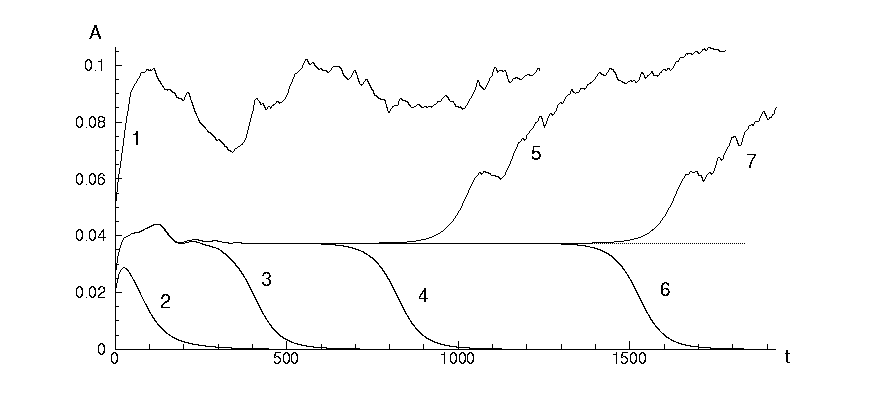
\includegraphics[width=1\linewidth]{bisection.png}}
\caption{Итерационный процесс построения решения на сепаратрисе. 1--7 --- эволюция среднеквадратичной амплитуды возмущений $A(t)$ при уточнении значения $\alpha$.}
\label{bisection_pic}
\end{figure}

С каждой новой итерацией решение проводит на сепаратрисе в среднем на 30 единиц времени больше. В расчетах для представления действительных числе использованы 64-битные числа с плавающей запятой. Это позволило найти около 50 приближений к решению на сепаратрисе. Соответственно, решение удалось удержать на сепаратрисе в течении приблизительно 1500 единиц времени. Из них ориентировочно первые 500 единиц происходит перестройка решения, после чего режим течения устанавливается. В согласии с результатами \cite{Avila2013}, решение на сепаратрисе при $\Re=2200$ постепенно выходит на условно периодический режим. Это решение описывает локализованной в пространстве структуры, которая сносится вниз по потоку с постоянной скоростью. В подвижной системе отсчета поле скорости в каждой точке испытывает периодические колебания. Для скорости сноса и периода колебаний получены значения $c=0.69$ и $T=60$ (в \cite{Avila2013} сообщается о $c=0.76$ и $T=60$). Во всех выполненных расчетах режим течения, устанавливающийся на сепаратрисе, не зависит от исходного турбулентного поля скорости $\v_{turb}$. 

\begin{comment}
Так как скорость сноса модельного порыва заранее не известна, решение на сепаратрисе было найдено в системе отсчета, двигающейся со скоростью $0.5$. После того, как решение на сепаратрисе найдено, изменить скорость перемещения системы отсчета уже не представляется возможным вследствие высокой чувствительности решения к возмущениям, возникающим в данном случае в результате неточностей численного интегрирования. Чтобы получить решение в сопутствующей системе отсчета, метод поиска решения на сепаратрисе применен повторно в системе отсчета, двигающейся с уже известной скоростью перемещения порыва. 
\end{comment}

Сравнение предельного решения на сепаратрисе с турбулентным порывом, представленное на рисунке \ref{3D_img}, показывает качественное согласие этих решений. Во всех структурах имеются протяженные области ускоренного и замедленного движения, концентрирующиеся в пристенной области трубы. Сохраняется и основная качественная особенность порыва --- медленное понижение осевой скорости на переднем фронте и более резкое её восстановление на заднем (смотри рисунок \ref{ucl_cmp_img}). Мы будем называть предельное решение на сепаратрисе {\it модельным порывом}.  

\begin{figure}
\center{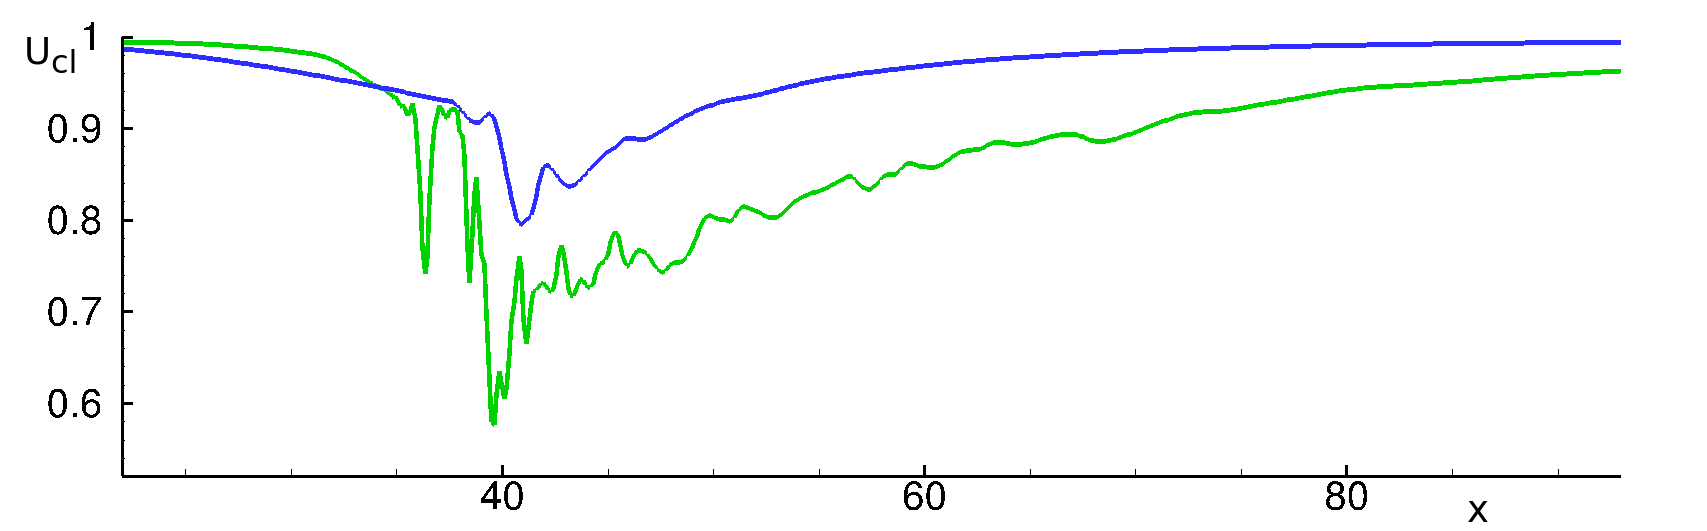
\includegraphics[width=0.7\linewidth]{ucl_cmp.png}}
\caption{Сравнение скорости на оси трубы в турбулентном (1) и модельном (2) порывах.}
\label{ucl_cmp_img}
\end{figure}

Для того, чтобы установить влияние условия периодичности вдоль трубы на предельное решение, решение было найдено в расчетной области вдвое большей протяженности, при $L_x = 160$ (число узлов сетки в продольном направлении также удвоено). Также при исходном значении $L_x = 80$ решение было получено на более подробной сетке, содержащей $1024 \times 64 \times 64$ ячеек (в сравнении с исходной сеткой в каждом направлении число ячеек удвоено). Результаты, полученные на трех сетках, качественно совпадают и количественно близки. Для сравнения, на рисунке \ref{amp_pic} представлены некоторые интегральные характеристики модельного порыва, полученные на различных сетках (подробное описание изображенных величин приведено в следующем разделе). Полученные результаты подтверждают достаточность расчетной сетки и длины расчетной области для адекватного воспроизведения модельного порыва, а также то, что его пространственная локализация не связана с условием периодичности вдоль трубы. Характеристики полученного модельного порыва согласуются с результатами работы \cite{Avila2013}. Это подтверждает, что найденное решение является решением математической задачи и не зависит от численного метода, которым оно было найдено. В работе \cite{Avila2013} решение получено двумя методами --- полностью спектральным \cite{Meseguer2007} и спектрально-конечно-разностным \cite{Willis2009}. Мы применяем конечно-разностный метод \cite{Nikitin2006}. Также, модельный порыв был воспроизведен в работе \cite{Chantry2014} спектрально-конечно-разностным методом \cite{Willis2009}; авторами также сообщается о совпадении результатов с \cite{Avila2013}. 


\section{Основные свойства модельного порыва} \label{edge_char_seq}

При $\Re=2200$ модельный порыв имеет длину около $40R$ и перемещается вдоль трубы со скоростью $c = 0.69U$. В подвижной системе отсчета он является периодическим по времени с периодом $T = 60 R/U$. Характерным свойством модельного порыва является наличие вытянутых вдоль потока областей с повышенным и пониженным значением продольной компоненты скорости, чередующихся в угловом направлении (смотри рисунок \ref{3D_img}). Полосы повышенной скорости целиком расположены около стенки трубы, полосы замедления соединяются в единое целое в приосевой области вблизи переднего фронта. Наличие вытянутых вдоль потока полос ускоренного и замедленного движения --- характерное свойство любого пристенного турбулентного течения. Однако, в отличие от реальной турбулентности, где полосы случайно блуждают во времени и в пространстве, в рассматриваемом решении полосы сохраняют свое положение и форму, лишь слегка искажаясь периодическими колебаниями. 

\begin{figure}
\center{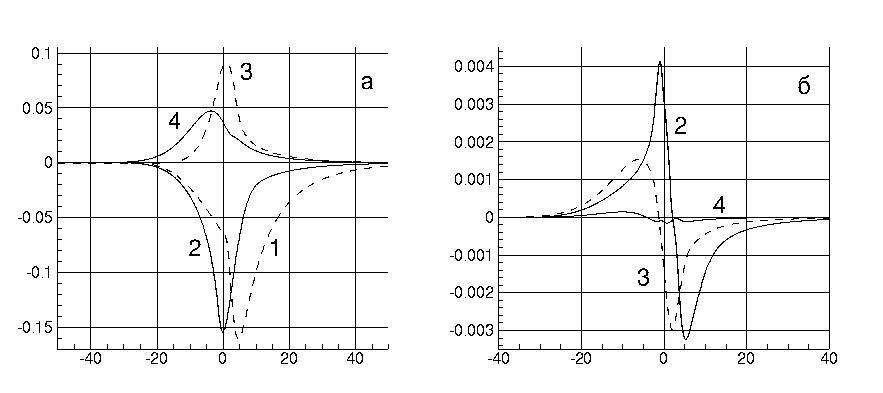
\includegraphics[width=1\linewidth]{U2D.png}}
\caption{Распределения вдоль трубы продольной (a) и радиальной (b) компоненты осесимметричной составляющей скорости $\V_{2D}$ для нескольких расстояний от оси трубы: 1–4 – r = 0, 0.4, 0.7, 0.9}
\label{U2D_pic}
\end{figure}

Для удобства перейдем в подвижную систему координат, перемещающуюся вдоль трубы со скоростью сноса локализованной структуры. В подвижной системе решение представляется в виде суперпозиции стационарной составляющей $\V(\x) = \overline{\v}^t$ и колебательной $\v_n(t,\x) = \v - \V$. Стационарную составляющую, в свою очередь, представим в виде суперпозиции осесимметричной $\V_{2D}(\x) = \overline{\V}^{\theta}$ и трехмерной $\V_{3D}(\x) = \V - \V_{2D}$ составляющих. Распределения продольной компоненты осесимметричной составляющей скорости вдоль трубы $V_{x,2D}(x)$ для нескольких расстояний от оси трубы представлены на рисунке \ref{U2D_pic}(а) (даны отклонения от течения Пуазейля). Начало системы отсчета $x=0$ помещено в сечение, в котором среднее отклонение скорости от течения Пуазейля максимально. Голова структуры, где начинает проявляться отклонение осевой скорости, располагается на расстоянии $x \approx 45$. Хвостовая часть структуры на сепаратрисе очерчена не так четко, как в турбулентных порывах, где восстановление скорости происходит на отрезке длиной в $3-5$ радиусов трубы.  Падение скорости в приосевой области трубы компенсируется ускорением у стенки. Поведение радиальной компоненты $V_{r,2D}$, показанное на рисунке \ref{U2D_pic}(b), соответствует изменению осевой скорости --- в зоне замедления на оси происходит растекание жидкости к стенкам, $V_{r,2D}>0$, в передней части происходит обратный процесс и $V_{r,2D}<0$.

\begin{figure}
\center{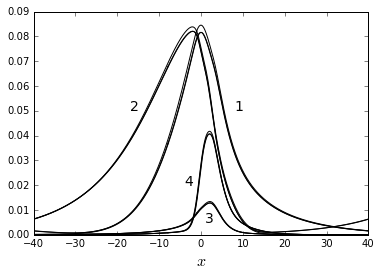
\includegraphics[width=0.6\linewidth]{amp.png}}
\caption{Распределения вдоль трубы среднеквадратичных по сечению амплитуд трех составляющих движения: 1 -- $\V_{2D}$ (отклонение от течения Пуазейля); 2, 3 -- продольная и поперечные компоненты скорости $\V_{3D}$; 4 -- $\v_{n}$. Представлены результаты, полученные на трех расчетных сетках, параметры которых приведены в разделе \ref{edge_seq}. }
\label{amp_pic}
\end{figure}

На рисунке \ref{amp_pic} приведены распределения по $x$ среднеквадратичных по сечению трубы амплитуд трех составляющих движения: стационарной осесимметричной (отклонение от течения Пуазейля) $A_{2D}$, стационарной трехмерной $A_{3D}$ и колебательной $A_n$. Распределение $A_{2D}(x)$ соответствует рисунку \ref{U2D_pic}. Отклонение от течения Пуазейля заметно на значительном отрезке от $x=-30$ до $x=40$. Максимум $A_{2D}$ составляет 8.4\%. Величина $A_{3D}$ характеризует интенсивность полосчатых структур. Как видно на рисунке~\ref{3D_img}, полосчатые структуры появляются на некотором расстоянии вверх по потоку от головы порыва и сохраняются на значительном расстоянии позади него. В соответствии с этим $A_{3D}(x)$ имеет выраженную асимметрию относительно точки $x=-2$, где эта величина достигает максимума. Интенсивность полос быстро падает вниз по потоку и сохраняется на значительном расстоянии в верхней части потока. В отличие от стационарных полосчатых структур, колебательная составляющая движения сосредоточена на сравнительно непротяженном отрезке трубы от $x=-5$ до $x=15$ с максимальной амплитудой в 4\% при $x=2.5$.


\begin{figure}[h]
\center{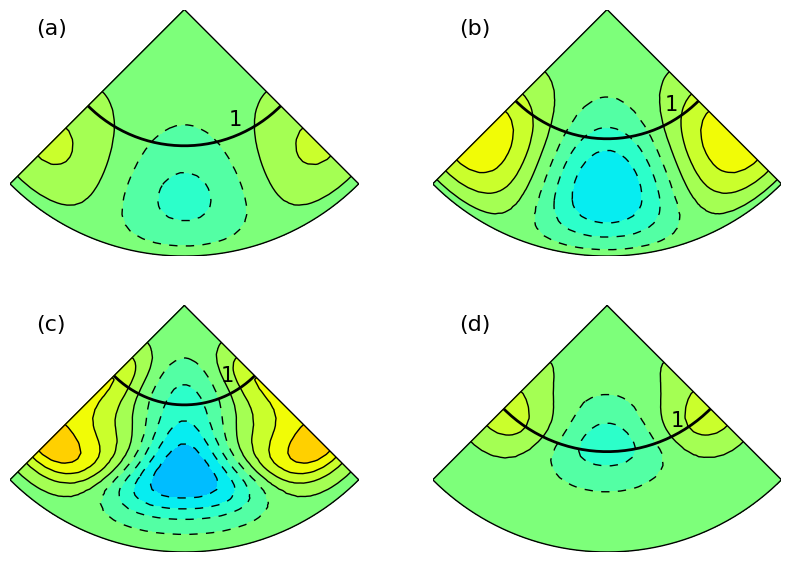
\includegraphics[width=0.8\linewidth]{V3D_cs.png}}
\caption{Распределения продольной составляющей $V_{x,3D}$ в нескольких сечениях трубы: (a)--(d) --- $x = -20, -10, 0, 5$. Сплошные изолинии --- положительная скорость, пунктирные изолинии --- отрицательная скорость, 1 --- линия, на которой относительная скорость жидкости равна нулю ($V_{x} = c$).}
\label{V3D_cs_pic}
\end{figure}


В трехмерную стационарную составляющую движения $\V_{3D}$ попадают полосы повышенной и пониженной скорости. Поле $V_{x,3D}$ в нескольких сечениях трубы изображено на рисунке~\ref{V3D_cs_pic}. В каждом сечении трубы полосы пониженной скорости ($V_{x,3D} < 0$) проходят через центр расчетной области, при $\theta = \pi/4$. Полосы повышенной скорости ($V_{x,3D} > 0$) попадают на границы расчетной области в угловом направлении, находящиеся при $\theta = 0, \pi/2$. Среднее поле скорости оказывается симметрично относительно плоскости, проходящей через центр расчетной области при $\theta = \pi/4$, так как поле скорости решения на сепаратрисе $\v = (v_x, v_r, v_\theta)$ имеет дополнительную симметрию отражения относительно указанной плоскости со сдвигом на половину периода по времени:
\begin{equation}
(v_x, v_r, v_\theta)(x, r, \pi/4 + \theta, t) = (v_x, v_r, -v_\theta)(x, r, \pi/4 - \theta, t + T/2). 
\end{equation} 


\begin{figure}[h]
\center{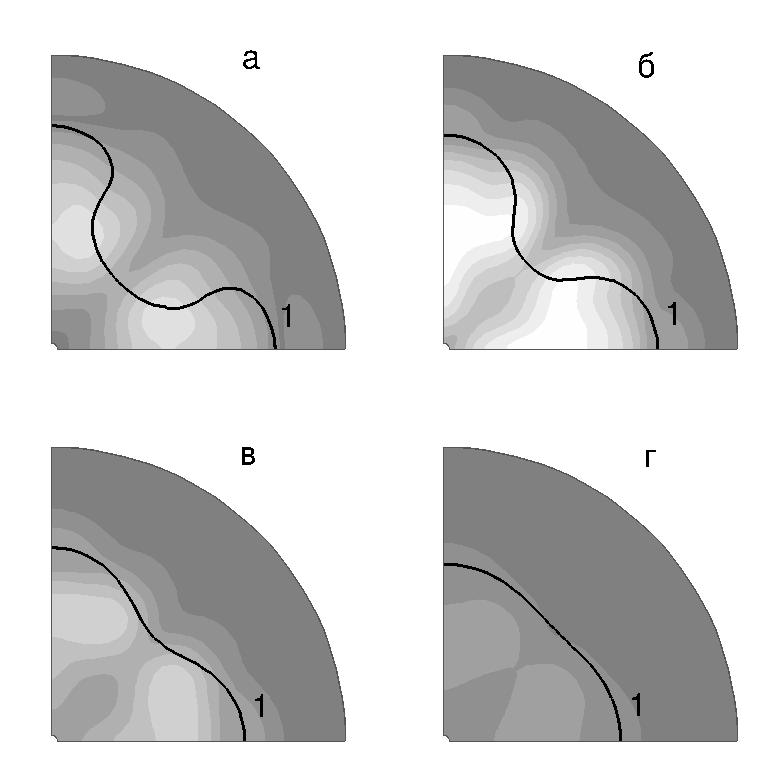
\includegraphics[width=0.8\linewidth]{puls_cs.png}}
\caption{Изолинии среднеквадратичной амплитуды колебаний в нескольких сечениях трубы: (a)--(d) --- x = 0, 2.5, 5, 7.5. В пристенной области амплитуда колебаний близка к нулю. 1 --- линия, на которой относительная скорость жидкости равна нулю ($V_{x} = c$).}
\label{puls_cs_pic}
\end{figure}

Распределения среднеквадратичной амплитуды пульсационной составляющей движения $\v_n$ в нескольких сечениях трубы приведены на рисунке \ref{puls_cs_pic}. Пульсации имеют существенную амплитуду между полосами повышенной и пониженной скорости, а также между полосой ускорения и осью трубы. Пульсационная составляющая движения $\v_n$ по форме напоминает бегущую волну. Её фазовая скорость близка к $0.77U$, что на $0.08U$ выше скорости перемещения порыва. Длина бегущей волны несколько меняется по мере продвижения вниз по потоку. Её можно оценить в $5R$. 


\section{Механизм поддержания полос повышенной и пониженной скорости} 

Все описанные составляющие движения находятся в динамическом взаимодействии друг с другом. Как видно на рисунке \ref{amp_pic} наиболее локализованной вдоль трубы оказывается колебательная составляющая. Доминирующая мода колебательной составляющей пропорциональна $e^{2\pi it/T}$ во времени и $e^{2i\theta}$ в угловом направлении. Нелинейное взаимодействие колебательных мод порождает колебания на высших частотах, а также дает вклад в стационарную составляющую движения. В стационарной составляющей кроме осесимметричной части доминирует мода, пропорциональная $e^{4i\theta}$, обладающая $\pi/2$-периодичностью в угловом направлении. Именно такой периодичности по углу соответствуют четыре пары полосчатых структур, наблюдающихся при решении задачи с условиями \eqref{sym_eq}, \eqref{per_eq}.

Отметим, что непосредственный вклад колебаний в образование полос не велик. Основной механизм роста полос это так называемый лифтап (<<lift-up>>) эффект, связанный с появлением движения в перпендикулярной к основному потоку плоскости. Частицы жидкости, перемещающиеся от стенки в сторону оси трубы, приносят дефект скорости и образуют полосу замедления, а частицы, двигающиеся в противоположном направлении --- от оси к стенке, образуют полосу ускорения. Основная роль колебательной составляющей в этом механизме состоит именно в порождении стационарного движения в поперечной плоскости, распределение среднеквадратичной амплитуды которого $A_{\perp}(x)$ также представлено на рисунке \ref{amp_pic} кривой 3. Как видно, область сосредоточения поперечного движения практически совпадает с областью существования колебаний. Некоторое уклонение $A_{\perp}(x)$ вверх по потоку объясняется конвективным переносом этого движения (поперечное движение в основном возникает в периферийной части сечения трубы, где скорость потока в выбранной системе отсчета отрицательна).

\begin{figure}[h]
\center{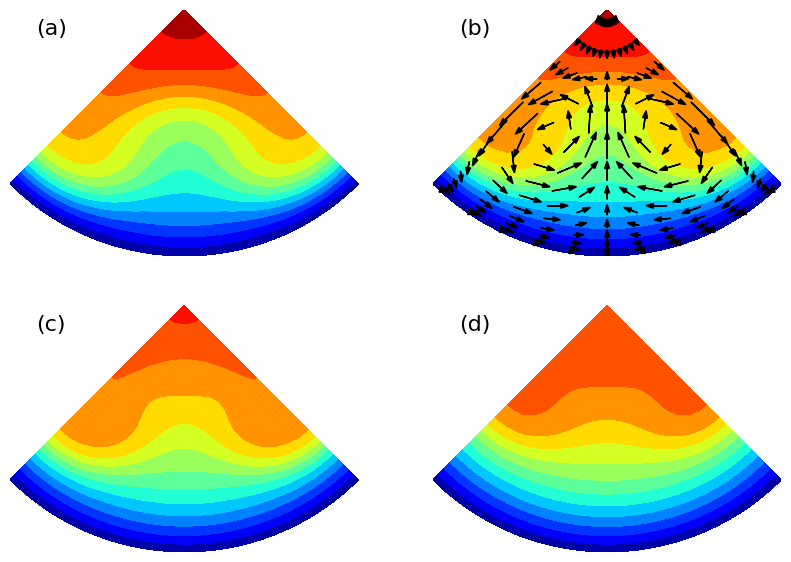
\includegraphics[width=1\linewidth]{VEL_cs.png}}
\caption{Среднее поле скорости $\V$: ряд (a) --- поперечная компонента, ряд~(b)~--- изолинии продольной компоненты. На стенке скорость жидкости равна нулю. Изображено три сечения трубы, $x = 0, 2.5, 5$.}
\label{VEL_cs_pic}
\end{figure}

На рисунке \ref{VEL_cs_pic} приведены поперечная $(V_r, V_\theta)$ и продольная $V_x$ компоненты стационарного течения в области, где пульсации имеют существенную амплитуду. Стационарное поперечное течение соответствует существованию в потоке стационарных продольных вихрей, поддерживающих существование полос. Там, где стационарное поперечное движение направлено от стенки к оси трубы, находятся полосы замедления. Там, где поперечное движение направлено к стенки --- полосы ускорения. 

Формирующиеся в области небольшой протяженности полосчатые структуры переносятся в переднюю и заднюю часть порыва за счет конвекции. На рисунке \ref{V3D_cs_pic} на линии 1 средняя продольная скорости $V_x$ в системе отсчета, связанной с порывом, равна нулю. В приосевой области, ограниченной этой линией, скорость положительна, а в периферийной --- отрицательна. Видно, что полосчатые структуры во всех сечениях (кроме переднего, x = 5) располагаются в области отрицательной относительной скорости. Среднее течение с отрицательной скоростью переносит полосчатые структуры в заднюю часть порыва, где они формируют картину, похожую на вытянутые щупальца медузы (смотри рисунок \ref{3D_img}). При $x > 5$ полосчатые структуры концентрируются в приосевой части трубы и конвектируются вперед положительной скоростью относительного движения, благодаря чему в передней части порыва $A_{3D}$ сохраняет заметную величину, несмотря на отсутствие поперечного движения.


\section{Механизм возбуждения пульсаций}

\begin{figure}
\center{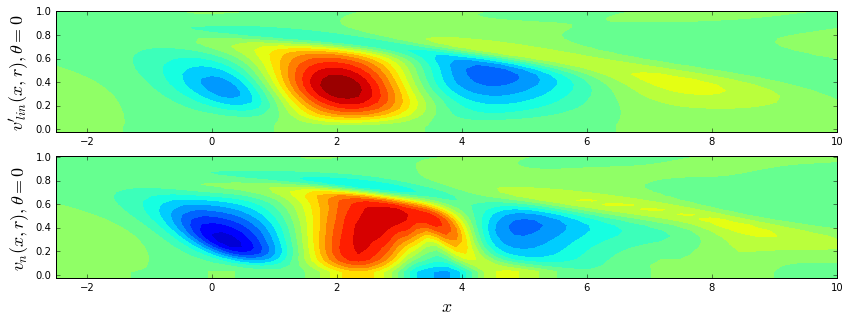
\includegraphics[width=1\linewidth]{lin_ls_cmp.png}}
\caption{Сравнение мгновенного поля продольной скорости пульсаций, возникающих в рамках линеаризованных уравнений, $\v'_1$ (a) и пульсационной составляющей движения $\v_n$ (b) в сечении $\theta = 0$. Сплошные изолинии --- положительные значения, прерывистые --- отрицательные.}
\label{lin_ls_cmp_pic}
\end{figure}

Полосчатые структуры достигают максимальной амплитуды в области $x\in[-5,0]$, где создаются условия для возникновения колебаний. Наиболее вероятный механизм генерации колебаний --- механизм потери устойчивости стационарной составляющей течения. Для проверки этой гипотезы стационарное течение $\V$ было исследовано на устойчивость к малым возмущениям $\v'$. Предположение малости $\v'$ позволяет линеаризовать уравнения. Линеаризованные относительно $\v'$ уравнения Навье-Стокса в подвижной системе координат, связанной с порывом, имеют вид:
\begin{equation} \label{lin_eq}
\frac{\partial \v'}{\partial t} = c \frac{\partial \v'}{\partial x} - (\V \cdot \nabla) \v' - (\v' \cdot \nabla) \V - \nabla p' + \nu \nabla^2 \v'. 
\end{equation}
Здесь $p'$ -- пульсационная составляющая давления. Расход $\v'$ равен нулю. Другие уравнения в постановке задачи линейные и для $\v'$ имеют тот же вид, что и для $\v$. Задача решается с дополнительными условия симметрии \eqref{sym_eq}, \eqref{per_eq}, которым удовлетворяет поле скорости модельного порыва. 

Линеаризованные относительно возмущений уравнения с некоторыми случайными начальными условиями интегрировались по времени до выхода решения на режим экспоненциального изменения. Обнаружено, что действительно поле скорости $\V$ неустойчиво к малым возмущениям. Растущее возмущение $\v'_1 \sim e^{(\lambda+i\omega)t}$ имеет инкремент нарастания $\lambda=0.012$ и частоту $\omega=0.116$, близкую к частоте колебаний $2\pi/60=0.105$ в решении на сепаратрисе. Что более существенно, поле скорости растущего решения $\v'_1$ качественно повторяет основные особенности поля скорости пульсационной составляющей движения модельного порыва $\v_n$. В качестве подтверждения на рисунке \ref{lin_ls_cmp_pic} представлены мгновенные поля скорости $\v'_1$ и $\v_n$ в продольном сечении $\theta = 0$. Моменты времени подобраны так, что фазы решений совпадают. Также на рисунке \ref{lin_amp_cmp_pic} для сравнения представлены амплитуды $\v_1'$ и $\v_n$ в нескольких сечениях трубы. Нет сомнений, что колебания возникают в результате линейной неустойчивости стационарной составляющей движения. Решение линейной задачи обладает дополнительной симметрией отражения относительно плоскости $\theta = \pi/4$, выражаемой формулой:
\begin{equation} \label{dop_sym_eq}
(-v_x, -v_r, v_\theta)(x, r, \pi/4 + \theta, t) = (v_x, v_r, v_\theta)(x, r, \pi/4 - \theta, t). 
\end{equation} 
В целом, поле $\v'_1$ имеет более простую форму, чем $\v_n$. В частности, $\v'_1$ меняется во времени по гармоническому закону. Простота формы $\v'_1$ делает его предпочтительным объектом при исследовании механизмов влияния пульсаций на среднее течение. 


\begin{figure}
\center{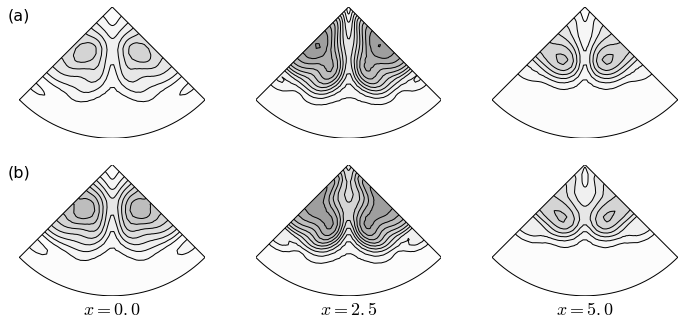
\includegraphics[width=1\linewidth]{lin_amp_cmp.png}}
\caption{Сравнение амплитуды пульсаций, возникающих в рамках линеаризованных уравнений, $\v'_1$ (ряд (a)) и пульсационной составляющей движения $\v_n$ (ряд (b)) в нескольких сечения трубы, $x = 0, 2.5, 5$. Вблизи стенки амплитуда пульсаций близка к нулю.}
\label{lin_amp_cmp_pic}
\end{figure}

В реальном течении пульсационная составляющая движения имеет конечную амплитуду и нелинейными слагаемыми в уравнении, описывающем эволюцию пульсаций, уже нельзя пренебрегать. По-видимому, роль нелинейных слагаемых сводится к тому, что они несколько меняют форму пульсаций так, что рост амплитуды пульсационной составляющей движения прекращается. При этом, именно линейные слагаемые определяют форму пульсаций и ответственны за передачу энергии в пульсационную составляющую движения. 

Отметим, что точки максимального роста колебаний находятся на линии, соответствующей нулевой относительной скорости (линия 1 на рис.~\ref{puls_cs_pic}). По этой причине область порождения колебаний остается неподвижной относительно порыва. Интересно, что в этой же области ($x = 0,\ r \approx 0.4$) происходит смена знака радиальной компоненты осесимметричной составляющей скорости (смотри рисунок~\ref{U2D_pic}(b)). При $x<0$ радиальная скорость положительна, поэтому колебания, возникшие в задней части порыва, относятся в сторону стенки трубы, где относительная скорость отрицательна, и продолжают двигаться вверх по течению. Наоборот, при $x>0$ радиальная скорость направлена к оси трубы. Туда же, в область положительной скорости, сносятся и колебания, обнаруживающиеся в передней части порыва.

Отметим также, что неустойчивость полосчатых структур является неотъемлемой составляющей всех сценариев самоподдержания турбулентности в пристенных течениях. В некоторых работах предполагается, что неустойчивость возникает в пристенных областях полос замедленного движения, где в локальном профиле скорости $V_x(r)$ на фоне наибольшего градиента появляется точка перегиба --- источник неустойчивости в механизме типа Кельвина--Гельмгольца. В частности, именно такой механизм предлагается в качестве механизма возникновения колебаний в турбулентном порыве в \cite{Shimizu2009}. В рассматриваемом нами решении на сепаратрисе это определенно не так. Как видно на рисунке~\ref{puls_cs_pic} в сечении $x=0$, соответствующем максимальной скорости роста колебаний, амплитуда колебаний минимальна как раз в области полосы замедления ($\theta=\pi/4$). Наибольшие колебания развиваются наоборот вблизи полос ускорения, а если быть более точным, в промежуточных областях между полосами. В этих областях стационарная составляющая скорости течения претерпевает наибольшее изменение и имеет точки перегиба, но не как функция радиальной переменной, а как функция угла.



\section{Влияние продольной неоднородности стационарной составляющей движения на форму пульсаций}

Замечено, что в модельном порыве область наибольшей интенсивности пульсаций совпадает с областью резкого падения скорости на его заднем фронте (см. рис. \ref{ucl_cmp_img}, \ref{amp_pic}). Аналогичная особенность отмечена в турбулентном порыве \cite{Hof2010}. Чтобы оценить роль продольной неоднородности среднего течения в процессе формирования пульсаций, в работе выполнен анализ устойчивости однородных вдоль трубы полей скорости $\U_i = \V\big|_{x=x_i}$, повторяющих среднее поле скорости модельного порыва $\V$ в сечениях трубы $x = x_i$. Значения $x_i$, при которых было выполнено исследование поля скорости $\U_i$, принадлежат интервалу $(-8,4)$, где пульсационная составляющая движения получает энергию от среднего течения и имеет существенную амплитуду. Поля скорости $\U_i$ имеют полосчатую структуру и воспроизводят неоднородность среднего поля скорости по координатам $r$ и $\theta$, но теряют неоднородность среднего течения по координате $x$. Сравнение характеристик устойчивости полей скорости $\V$ и $\U_i$ позволяет делать выводы о роли продольной неоднородности в процессе формирования пульсаций. 

Собственные решения линейной задачи устойчивости однородного вдоль трубы поля скорости имеют вид $\v' = \mathrm{Real}\left(\hat \v (r, \theta, t) e^{i \alpha x}\right)$, где функция $\hat \v$ имеет комплексные значения, функция $\mathrm{Real}(z)$ имеет значение действительной части комплексного числа $z$. Постановка задачи линейной устойчивости однородного вдоль трубы поля скорости формулируется относительно $\hat \v$ и является двумерной (пропадает зависимость от $x$). Задача имеет дополнительный параметр $\alpha > 0$, характеризующий волновое число возмущения, устойчивость к которому анализируется. В этой постановке уравнения движения в системе координат, перемещающейся вдоль трубы со скоростью $c$, и уравнение неразрывности имеют вид: 
\begin{equation} \label{hat_NS_eq}
\frac{\partial \hat \v}{\partial t} = i \alpha  c \hat \v - (\U_i \cdot \hat \nabla) \hat \v - (\hat \v \cdot \nabla) \U_i - \hat \nabla \hat p + \nu \hat \nabla^2 \hat \v,
\end{equation}
\begin{equation} \label{hat_div_eq}
\hat \nabla \cdot \hat \v = 0,
\end{equation}
где функция $\hat p = \hat p(r,\theta,t)$ имеет комплексные значения, $p' = \mathrm{Real}\left(\hat p e^{i \alpha x}\right)$ --- пульсационная составляющая давления, оператор $\hat \nabla$ имеет вид: 
\begin{equation*}
\hat \nabla = \left( i\alpha, \frac{\partial}{\partial r}, \frac{\partial}{r \partial \theta} \right).
\end{equation*}
На стенках трубы ставится условие прилипания. На решение накладываются дополнительные условия симметрии \eqref{sym_eq}, \eqref{per_eq}, при которых найден модельный порыва. Условие периодичности вдоль потока \eqref{bc2_eq} снимается. 

\begin{figure}
\center{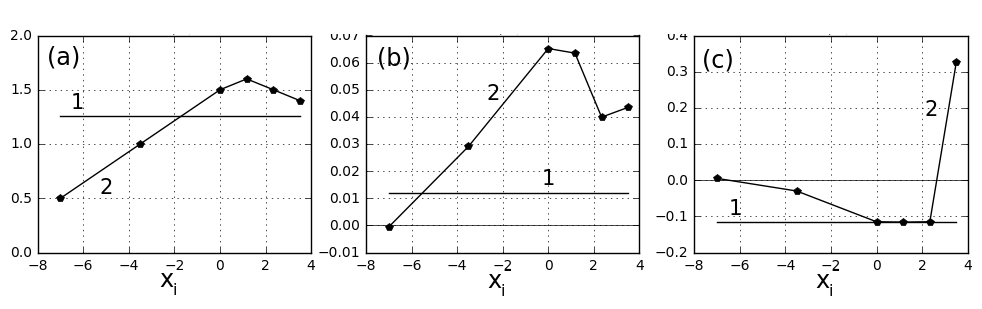
\includegraphics[width=1\linewidth]{cs_lin.png}}
\caption{Значение волнового числа $\alpha$ (a), инкремента нарастания $\lambda$ (b) и угловой частоты $\omega$ (в системе отсчета порыва) (c) для наиболее быстро растущего возмущения поля скорости модельного порыва $\V$ (линия 1) и однородных вдоль потока полей скорости $\U_i$, повторяющих $\V$ в сечении $x = x_i$ (точки на линии 2).}
\label{cs_lin_pic}
\end{figure}

На устойчивость исследованы поля скорости $\U_i = \V\big|_{x=x_i}$ для $x_i = -7.1,$ $-3.5, 0, 1.2, 2.3, 3.5$.  Для каждого исследованного $\U_i$ среди собственных решений линейной задачи устойчивости с различными значениями волнового числа $\alpha >0$ найдено наиболее быстро растущее (медленно затухающее). Наиболее быстро растущее (медленно затухающее) собственное решение линейной задачи устойчивости поля скорости $\U_i$ при фиксированном значении $\alpha$ получено интегрированием уравнений \eqref{hat_NS_eq}, \eqref{hat_div_eq} со случайными начальными данными до выхода на экспоненциальный режим роста, $||\hat \v|| \sim e^{(\lambda + i\omega) t}$. 

На рисунке \ref{cs_lin_pic} приведены полученные значения волнового числа $\alpha$, инкремента нарастания $\lambda$ и угловой частоты $\omega$ для наиболее быстро растущих (медленно затухающих) возмущений поля скорости $\U_i$, как функции $x_i$ (точки на линии 2). Также на рисунке (линией 1) приведены характеристики наиболее быстро растущего возмущения стационарной составляющей поля скорости модельного порыва $\V$ (значение длины волны приблизительное). Угловая частота приведена в системе отсчета, перемещающейся со скоростью порыва. 

Поля скорости $\U_i$ при $x_i \in (-4,4)$ оказываются неустойчивыми, причем скорость роста наиболее быстро растущего возмущения оказывается выше скорости роста возмущений стационарной составляющей движения модельного порыва $\V$. Наибольшей скоростью роста обладают возмущения полей скорости $\U_i$ при $x_i \in (0, 2)$. Следствием этого факта может быть то, что именно при $x \in (0,2)$ пульсационная составляющая движения $\v_n$ достигает наибольшей амплитуды (см. рис. \ref{amp_pic}). Наиболее быстро растущие  возмущения полей скорости $\U_i$ при $x_i \in (0,3)$ повторяют форму пульсационной составляющей движения модельного порыва. В частности, их волновые числа и угловые частоты близки к соответствующим значениям как для наиболее быстро растущих возмущений поля скорости $\V$, так и для пульсационной составляющей движения модельного порыва $\v_n$. Распределения по сечению трубы амплитуды колебаний для наиболее быстро растущих возмущений полей скорости $\U_i$ при $x_i \in (0,3)$, приведенные на рисунке \ref{cs_lin_map_pic}, повторяют распределение амплитуды колебаний в модельном порыве (см. рис. \ref{puls_cs_pic}).


\begin{figure}
\center{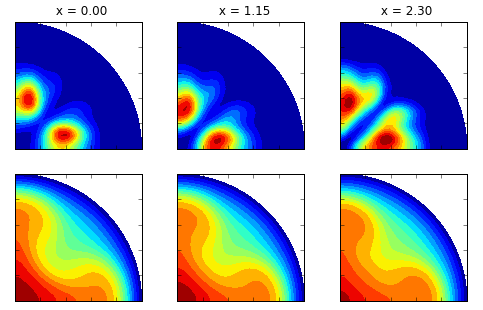
\includegraphics[width=1\linewidth]{cs_lin_map.png}}
\caption{Изолинии амплитуды колебаний для наиболее быстро растущего возмущения однородного вдоль трубы поля скорости $\U_i$ (a) и изолинии продольной компоненты поля скорости $\U_i$ (b), $x_i = 0, 1.2, 2.3$.}
\label{cs_lin_map_pic}
\end{figure}

Если при $x_i \in (0,3)$ наиболее быстро растущее возмущения полей скорости $\U_i$ повторяют качественные особенности пульсационной составляющей движения модельного порыва, то уже при $x_i = 3.5$ наиболее быстрорастущим оказывается возмущение принципиально другой формы. С этим, в частности, связано резкое отличие значения угловой частоты $\omega$, полученного при $x_i = 3.5$, от значений, полученных при меньших $x_i$ (см. рис. \ref{cs_lin_pic}). 

Среди исследованных однородных вдоль трубы полей скорости, имеющих полосчатую структур, найдены неустойчивые, для которых наиболее быстрорастущие возмущения воспроизводят как качественные, так и количественные характеристики пульсационной составляющей движения модельного порыва и имеют даже большую скорость роста, чем наиболее быстрорастущие возмущение средней составляющей движения модельного порыва. Таким образом, может быть сделан вывод, что продольная неоднородность стационарной составляющей движения не является необходимым условием для возникновения пульсаций. Образование пульсаций связано с неоднородностью стационарной составляющей движения в поперечной плоскости. 


\section{Взаимодействие между компонентами движения модельного порыва}

В предыдущих разделах были выделены компоненты движения модельного порыва и основные механизмы взаимодействия между ними. Компоненты движения находятся в динамическом равновесии, поддерживая существование друг друга и, следовательно, самого порыва. Более строго обосновать полученные результаты позволяет анализ баланса кинетической энергии в системе. Вклад каждой из компонент движения в производство кинетической энергии других компонент движения может быть вычислен на основе уравнений движения, и, в зависимости от его величины, могут быть сделаны выводы о положительном или отрицательном влиянии одних компонент движения на другие. 

Ниже приведен вывод уравнений баланса кинетической энергии для каждой компоненты движения. 
Осреднение уравнения Навье-Стокса по времени в системе отсчета, связанной с порывом, дает уравнение баланса импульса стационарной составляющей движения $\V = \overline{\v}^t$:
\begin{equation} \label{VEL_eq}
\pd{\V}{t} = c \pd{\V}{x} - (\V \cdot \nabla) \V - \overline{(\v_n \cdot \nabla) \v_n}^t - \nabla P + \nu \nabla^2 \V.
\end{equation}
Здесь $c$ --- скорость перемещения порыва, $P$ --- стационарная составляющая давления, $\v_n$ --- пульсационная составляющая скорости, черта над выражением с индексом $t$ обозначает осреднение по времени. Формально производная по времени от стационарной составляющей движения равна нулю, однако слагаемое $\partial \V/ \partial t$ сохранено в записи уравнения \eqref{VEL_eq} для удобства восприятия. В сравнении с уравнением Навье-Стокса в \eqref{VEL_eq} возникает новое слагаемое $-\overline{(\v_n, \nabla) \v_n}^t$, выражающее влияние пульсационной составляющей движения на среднее течение. 

Последующее осреднение \eqref{VEL_eq} по угловой координате дает уравнения баланса импульса двумерной компоненты движения $\V_{2D} = \overline{\V}^\theta$:
\begin{multline} \label{V2D_eq}
\pd{\V_{2D}}{t} = c \pd{\V_{2D}}{x} - (\V_{2D} \cdot \nabla) \V_{2D} - \overline{(\V_{3D} \cdot \nabla) \V_{3D}}^{\theta} - \overline{(\v_n \cdot \nabla) \v_n}^{t,\theta} - \\ - \nabla P_{2D} + \nu \nabla^2 \V_{2D}.
\end{multline}
Здесь $P_{2D} = \overline{P}^{\theta}$ --- двумерная составляющая давления, $\V_{3D} = \V - \V_{2D}$ --- трехмерная составляющая скорости, черта над выражением с индексом $\theta$ --- осреднение по угловой переменной. Вычитание \eqref{V2D_eq} из \eqref{VEL_eq} дает уравнение баланса импульса трехмерной составляющей движения $\V_{3D}$:
\begin{multline} \label{V3D_eq}
\pd{\V_{3D}}{t} = c \pd{\V_{3D}}{x} - (\V_{3D} \cdot \nabla) \V_{3D} - (\V_{3D} \cdot \nabla) \V_{2D} - (\V_{2D} \cdot \nabla) \V_{3D} + \\ + \overline{(\V_{3D} \cdot \nabla) \V_{3D}}^{\theta} - \overline{(\v_n \cdot \nabla) \v_n}^{t} + \overline{(\v_n \cdot \nabla) \v_n}^{t, \theta} - \nabla P_{3D} + \nu \nabla^2 \V_{3D}.
\end{multline}
Здесь $P_{3D} = P - P_{2D}$ --- трехмерная составляющая давления. Проектирование уравнения \eqref{V3D_eq} на ось $x$ дает уравнение, описывающее баланс импульса составляющей движения $\V_S = (V_{x,3D}, 0, 0)$, ассоциированной с полосами повышенной и пониженной скорости. Проектирование уравнения \eqref{V3D_eq} на поперечное сечение трубы дает уравнение баланса импульса составляющей движения $\V_V = (0, V_{r,3D}, V_{\theta,3D})$, ассоциированной с продольными вихрями. 
%Стоит отметить, что $\V_{2D}, \V_{3D}, \v_n$ удовлетворяют условию несжимаемости \eqref{eq0_Re}, в то время как $\V_S$ и $\V_V$ не удовлетворяют ему. 

\begin{figure}
\center{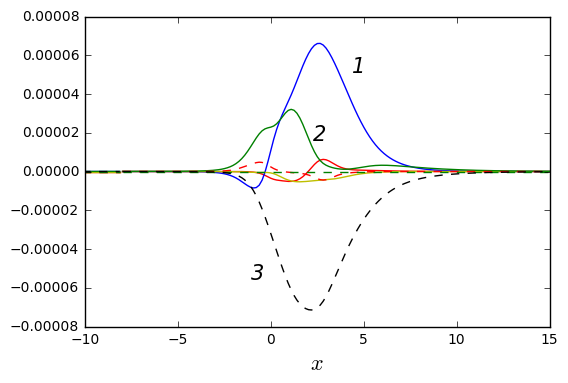
\includegraphics[width=0.6\linewidth]{e1_parts.png}}
\caption{Вклад в производство кинетической энергии пульсационной составляющей движения со стороны: 1 --- $\V_S$; 2 --- $\V_{2D}$; 3 --- вязких слагаемых. Другие слагаемые существенного вклада не дают.}
\label{e1_parts_pic}
\end{figure}

Вычитание \eqref{VEL_eq} из \eqref{NS_eq} дает уравнение эволюции пульсационной составляющей движения $\v_n$: 
\begin{multline} \label{vel1_eq}
\pd{\v_n}{t} = c \pd{\v_n}{x} - (\v_n \cdot \nabla) \v_n + \overline{(\v_n \cdot \nabla) \v_n}^t - (\V_{2D} \cdot \nabla) \v_n - (\V_S \cdot \nabla) \v_n - (\V_V \cdot \nabla) \v_n - \\ - (\v_n \cdot \nabla) \V_{2D} - (\v_n \cdot \nabla) \V_S - (\v_n \cdot \nabla) \V_V - \nabla p_n + \nu \nabla^2 \v_n. 
\end{multline}
Здесь $p_n = p - P$ --- пульсационная составляющая давления, среднее поле скорости представлено в виде суммы компонент движения $\V = \V_{2D} + \V_S + \V_V$, которые оказывают влияние на пульсационную составляющую движения через соответствующие нелинейные слагаемые. Осреднение по времени \eqref{vel1_eq}, умноженного на $\v_n$, дает уравнение изменения кинетической энергии пульсационной составляющей движения $e_n = \overline{\v_n^2/2}^t$: 
\begin{equation}\label{en_eq}
\pd{e_n}{t} = D_n^{2D} + D_n^{S} + D_n^{V} - \overline{\v_n (\v_n \cdot \nabla) \v_n}^t - \overline{\v_n \cdot \nabla p_n}^t + \nu \overline{\v_n \cdot \nabla^2 \v_n}^t,
\end{equation}
где слагаемые $D_n^{2D}$, $D_n^{S}$ и $D_n^{V}$ выражают генерацию $e_n$, обусловленную нелинейным взаимодействием $\v_n$ с компонентами движения $\V_{2D}$, $\V_S$ и $\V_V$, соответственно. Значения $D_n^{2D}$, $D_n^{S}$, $D_n^{V}$ вычисляются по формулам:
$$
D_n^{2D} = c \pd{e_n}{x}  - (\V_{2D} \cdot \nabla) e_n - \overline{\v_n (\v_n \cdot \nabla) }^t \V_{2D},
$$
$$
D_n^{S}  = - (\V_S \cdot \nabla) e_n - \overline{\v_n (\v_n \cdot \nabla)}^t \V_S,
$$
$$
D_n^{V} =  - (\V_V \cdot \nabla) e_n - \overline{\v_n (\v_n \cdot \nabla)}^t \V_V.
$$

На рисунке \ref{e1_parts_pic} приведены графики усреднённых по сечению трубы слагаемых из правой части уравнения \eqref{en_eq}. Наибольший вклад в генерацию кинетической энергии пульсаций $e_n$ дает слагаемое $D_n^S$ (кривая 1), что согласуется с представлениями о возникновении пульсаций вследствие линейной неустойчивости полосчатого движения. Хотя и не определяющий, но существенный положительный вклад дает слагаемое $D_n^{2D}$ (кривая 2). Так как течение $e_n$ не меняется во времен, сумма всех слагаемых в правой части уравнения \eqref{en_eq} равна нулю. Положительный вклад в генерацию $e_n$ со стороны $D_n^S$ и $D_n^{2D}$ компенсируется вязким слагаемым (кривая 3). Влияние других слагаемых оказывается незначительным. 

\begin{figure}
\center{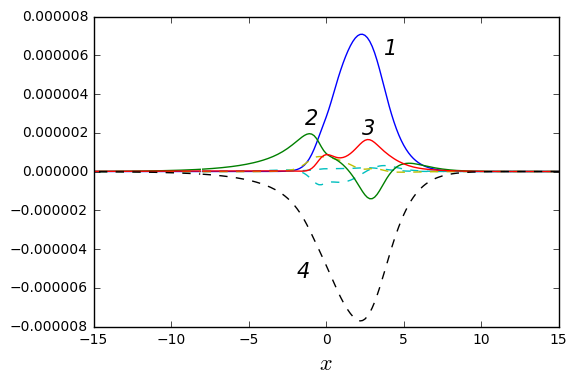
\includegraphics[width=0.6\linewidth]{ev_parts.png}}
\caption{Вклад в производство кинетической энергии движения $\V_V$, ассоциированного с продольными вихрями, со стороны: 1 --- $\v_n$; 2 --- $\V_{2D}$; 3 --- градиента давления; 4 --- вязких слагаемых. Другие слагаемые существенного вклада не дают.}
\label{ev_parts_pic}
\end{figure}

Аналогично, осреднение по $\theta$ уравнения \eqref{V3D_eq}, умноженного на поле скорости $\V_V$, ассоциированного с продольными вихрями, дает уравнение баланса кинетической энергии $E_V = \overline{\V_V^2/2}^\theta$:
\begin{equation}\label{EV_eq}
\pd{E_V}{t} = D_V^{2D} + D_V^{2D,S} + D_V^{S} + D_V^n - \overline{\V_V (\V_V \cdot \nabla) \V_V}^\theta - \overline{\V_V \nabla P_{3D}}^\theta + \nu \overline{\V_V \nabla^2 \V_V}^\theta,
\end{equation}
где слагаемые $D_V^{2D}$, $D_V^{2D,S}$, $D_V^S$, $D_V^n$ описывают влияние на поле скорости $\v_n$ компонент движения $\V_{2D}$, $\V_S$, $\V_n$, обусловленное нелинейным взаимодействие между ними. Значения $D_V^{2D}$, $D_V^{2D,S}$, $D_V^S$, $D_V^n$ вычисляются по формулам:
$$
D_V^{2D} = c \pd{E_V}{x} - (\V_{2D} \cdot \nabla) E_V - \overline{\V_V (\V_V \cdot \nabla)}^\theta \V_{2D},
$$
$$
D_V^{2D,S} = - \overline{\V_V (\V_S \cdot \nabla)}^\theta \V_{2D},
$$
$$
D_V^{S} = - \overline{\V_V (\V_S \cdot \nabla) \V_V}^\theta,
$$
$$
D_V^n = - \overline{\V_V (\v_n \cdot \nabla) \v_n}^{t,\theta}.
$$

Графики усредненных по сечению трубы слагаемых правой части уравнения \eqref{EV_eq} приведены на рисунке \ref{ev_parts_pic}. В соответствии с общими представлениями, наибольший вклад в производство продольных вихрей дает пульсационная составляющая движения. Её вклад в образование кинетической энергии $E_V$ выражает слагаемое $D_V^n$ (линия 1). Также существенный положительный вклад дает градиент давления, однако его интегральный вклад ниже почти в $5$ раз (линия 3). Слагаемое, выражающее вклад градиента давления в производство $E_V$, отлично от нуля, так как поле скорости $\V_V$ не соленоидальное. Также можно отметить влияние $\V_{2D}$, выраженное слагаемым $D_V^{2D}$ (линия 2). При $x > 0$ оно отрицательно, а при $x < 0$ --- положительно. Такое поведение соответствует тому, что продольная завихренность, формирующейся при положительных $x$, сносится вверх по течению вместе с основным потоком вблизи стенки за счет конвекции. Производство кинетической энергии $E_V$ перечисленными слагаемыми компенсируется вязким слагаемым (линия 4). Другие слагаемые в уравнении \eqref{EV_eq} существенного влияния не оказывают. 

\begin{figure}
\center{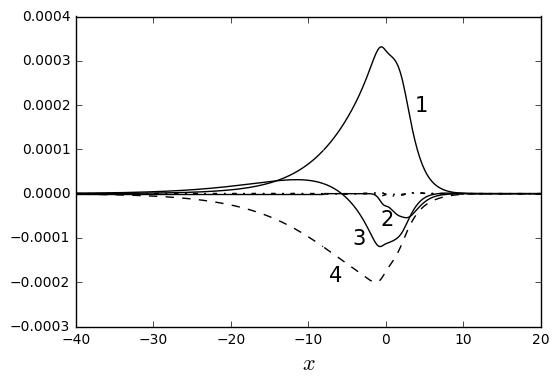
\includegraphics[width=0.6\linewidth]{es_parts.png}}
\caption{Вклад в кинетическую энергию движения $\V_S$, ассоциированного с полосами, со стороны: 1 --- $\V_V$ и $\V_{2D}$; 2 --- $\v_n$; 3 --- $\V_{2D}$; 4 --- вязких слагаемых. Другие слагаемые существенного вклада не дают.}
\label{es_parts_pic}
\end{figure}

Осреднение по переменной $\theta$ уравнения \eqref{V3D_eq}, умноженного на поле скорости $\V_S$,  ассоциированное с полосами, дает уравнение баланса кинетической энергии $E_S = \overline{\V_S^2/2}^\theta$:
\begin{equation}\label{ES_eq}
\pd{E_S}{t} = D_S^{2D} + D_S^{2D,V} + D_S^V + D_S^n - \overline{\V_S (\V_S \cdot \nabla) \V_S}^\theta - \overline{\V_S \nabla P_{3D}}^\theta + \nu \overline{\V_S \nabla^2 \V_S}^\theta.
\end{equation} 
Слагаемые $D_S^{2D}$, $D_S^{2D,V}$, $D_S^V$, $D_S^n$ вычисляются по формулам:
$$
D_S^{2D} = c \pd{E_S}{x} - (\V_{2D} \cdot \nabla) E_S - \overline{\V_S (\V_S \cdot \nabla)}^\theta \V_{2D},
$$
$$
D_S^{2D,V} = - \overline{\V_S (\V_V \cdot \nabla)}^\theta \V_{2D},
$$
$$
D_S^{V} = - \overline{\V_S (\V_V \cdot \nabla) \V_S}^\theta,
$$
$$
D_S^n = - \overline{\V_S (\v_n \cdot \nabla) \v_n}^{t,\theta}.
$$

Графики усредненных по сечению трубы слагаемых правой части уравнения \eqref{ES_eq} приведены на рисунке \ref{es_parts_pic}. В этом случае наибольший вклад дает слагаемое $D_S^{2D,V}$ (линия 1). Оно выражает совместное влияние на $\V_S$ со стороны компонент движения $\V_{2D}$ и $\V_V$ и в скалярных переменных имеет вид:
$$
D_S^{2D,V} =  - V_{x, S} V_{r, V} \pd{V_{x, 2D}}{r}.
$$
Доминирующая роль этого слагаемого согласуется с представлением о том, что продольные вихри формируются за счет <<лифт-ап>> эффекта. Нормальной к стенке трехмерная компонента скорости $V_{r,V} = V_{r,3D}$ перераспределяет продольный импульс двумерного основного течения $V_{x, 2D}$, образуя тем самым трехмерную составляющую продольной скорости $V_{x,3D} = V_{x,S}$. Пульсации оказывают небольшое отрицательное влияние на формирование полос (линия 2). Двумерное течение оказывает отрицательное влияние вблизи нуля, в то время, как в задней части порыва, при $x \sim -10$, его влияние оказывается положительным (линия 3). По-видимому, это связанно с конвективным переносом полос, формирующихся в передней части порыва, в его заднюю часть вблизи стенки, осуществляемое основным течением $\V_{2D}$. Получаемая составляющей движения $\V_S$ энергия компенсируется вязким слагаемым (линия 4). Другие слагаемые существенного влияния не оказывают. 

Полученные в разделе результаты подтверждают существующие представления о взаимодействии между компонентами движения модельного порыва. Также полученные результаты указывают на то, что все существенные взаимодействия между компонентами движения выделены и учтены. Данные о производстве кинетической энергии двумерной компоненты движения в разделе не приведены. За поддержание двумерного течения ответственен внешний перепад давления. Производимая внешним перепадом давления кинетическая энергия компенсируется вязкими слагаемыми. 



\section{Выводы по главе}

В главе представлены результаты численного исследования модельного порыва. Соответствующее модельному порыву решение уравнений Навье-Стокса является предельным состоянием решения, эволюционирующего на сепаратрисе, отделяющей в фазовом пространстве области притяжения решений, соответствующих ламинарному и турбулентному режимам течения. Предельное решение на сепаратрисе описывает локализованную в пространстве структуру, перемещающуюся вниз по потоку с постоянной скоростью. В сопутствующей системе отсчета при наложенных условиях симметрии оно оказывается периодическим по времени. Модельный порыв воспроизводит некоторые характерные особенности турбулентного порыва, а простота временного поведения позволяет выполнить его подробное исследование. Мы полагаем, что исследование модельного порыва может помочь приблизиться к пониманию турбулентного порыва.

При изучении модельного порыва установлены его основные характеристики, такие как скорость перемещения вдоль трубы и период изменения во времени. Составлено представление о внутренней структуре модельного порыва и выделены основные элементы цикла поддержания колебаний. Осреднение по времени в сопутствующей системе отсчета позволило разделить поле скорости модельного порыва на среднюю и пульсационную составляющие. Характерной особенностью среднего течения является наличие вытянутых вдоль трубы полос --- областей, скорость жидкости внутри которых существенно выше или ниже среднего значения. Полосы повышенной и пониженной скорости чередуются в угловом направлении. Показано, что пульсационная составляющая движения возникает в результате линейной неустойчивости среднего течения. Вероятным механизмом образования пульсаций является механизм типа Кельвина-Гельмгольца, так как пульсации возникают в области между полосами повышенной и пониженной скорости, где в среднем течении находятся точки перегиба, если рассматривать его как функцию угловой переменной. Изменение среднего течения вдоль оси $x$ существенного влияния на формирование пульсаций не оказывает. Показано, что полосы образуются за счет так называемого <<лифт-ап>> эффекта. В течении существуют стационарные продольные вихри, перемещающие жидкость в нормальной к основному потоку плоскости. Там, где медленная жидкость перемещается от стенки в основной поток, образуются полосы пониженной скорости. Между полосами пониженной скорости, где жидкость перемещается ближе к стенке, формируются полосы повышенной скорости. Формируясь в области небольшой протяженности, полосы вытягиваются вверх по потоку за счет конвекции. Полученные результаты позволяют сделать вывод о том, что поддержание стационарных продольных вихрей связано с наличием пульсаций. Такое представление подтверждается в следующей главе, посвященной механизму образования продольных вихрей.

Согласованность результатов, полученных на нескольких расчетных сетках, между собой и с результатами других авторов позволяет сделать вывод о том, что полученное предельное решение на сепаратрисе является решением уравнений Навье-Стокса и не зависит от выбора численного метода, которым оно было получено, и параметров расчета.

Выделенный в работе механизм поддержания модельного порыва согласуется с существующими представлениями о поддержании организованных структур в пристенных турбулентных течениях \cite{Hamilton1995, Waleffe1995, Waleffe1997, Jimenez1999, Schoppa2002}. Основным элементом организованных структур являются полосы повышенно и пониженной скорости, наблюдающиеся в буферном слое \cite{Kline1967, Smith1983}. Полосы в турбулентном течении перемещаются вдоль стенки и имеют ограниченное время жизни, но они достаточно хорошо различимы на фоне мелкомасштабных турбулентных пульсаций. Образование пульсаций в потоке связывают с неустойчивостью сдвиговых слоев, присутствующих в полосчатом течении. В работе \cite{Kim1971} сделан вывод о том, что производство турбулентных пульсаций в пристенных течениях практически полностью обусловлено периодически повторяющемся взрывообразным развитием неустойчивости на полосах пониженной скорости (<<bursting phenomenon>>). Считается, что полосы образуются за счет <<лифт-ап>> эффекта, но механизм образования продольных вихрей до сих пор не установлен. 



 

%[2] Kline, S. J., Reynolds, W. C., Schraub, F. A. & Runstadler, P. W. 1967 The structure of turbulent boundary layers. J. Fluid Mech. 30, 741–773.

%[19] Smith, C. R. & Metzler, S. P. 1983 The characteristics of low-speed streaks in the near-wall region of a turbulent boundary layer. J. Fluid Mech. 129, 27–54.

%[20] Kim, H. T., Kline, S. J. & Reynolds, W. C. 1971 The production of turbulence near a smooth wall in a turbulent boundary layers. J. Fluid Mech. 50, 133–160.

%[21] Hamilton, K., Kim, J. & Waleffe, F. 1995 Regeneration mechanisms of near-wall turbulence structures. J. Fluid Mech. 287, 317–348.
%[22] Jimenez, J. & Pinelli, A. 1999 The autonomous cycle of near wall turbulence. J. Fluid Mech. 389, 335–359.
%[23] Schoppa, W. & Hussain, F. 2002 Coherent structure generation in near-wall turbulence. J. Fluid Mech. 453, 57–108.
%[24] Waleffe, F. 1995 Hydrodynamic stability and turbulence: Beyond transients to a self-sustaining process. Stud. Appl. Maths 95, 319–343.
%[25] Waleffe, F. 1997 On a self-sustaining process in shear flows. Phys. Fluids 9, 883–900.













\chapter{Механизм поддержания продольных вихрей}


В предыдущей главе описан метод получения модельного порыва и его основные характеристики. Механизм самоподдержания модельного порыва оказывается связан с бегущей волной, которая может быть в нем выделена. Длина бегущей волны приблизительно равна 5 радиусам трубы $R$. Автором работы было обнаружено, что при условии $5R$ периодичности вдоль трубы метод поиска решения на сепаратрисе дает точную бегущую волну. Она повторяет основные особенности бегущей волны, наблюдаемой в модельном порыве, но является стационарной в сопутствующей системе отсчета. Простота поведения найденного решения позволила выделить нелинейный механизм взаимодействия пульсаций, ответственный за формирование продольных вихрей, и в строгом виде продемонстрировать ряд особенностей движения, обеспечивающих его работу. В этой главе представлены результаты исследования найденной бегущей волны и их обобщение на модельный порыв. 



\section{Характеристики возникающей на сепаратрисе бегущей волны}

Применение метода поиска решения на сепаратрисе, описанного в разделе \ref{edge_seq}, в расчетной области небольшой протяженности при $L_x = 5$, $\Re = 2200$ позволило получить решение типа нелинейной бегущей волны. Возникающая бегущая волна повторяет особенности бегущей волны, наблюдаемой в модельном порыве, однако, в отличии от нее, является точной в том смысле, что её поле скорости строго периодично вдоль трубы и во времени. В сопутствующей системе отсчета новое решение оказывается стационарным, что делает его более доступным для исследования. Фазовая скорость найденной бегущей волны равна $c_{tw} = 0.77$ (<<traveling wave>>), что соответствует скорости перемещения бегущей волны в модельном порыве. Возможно, найденная бегущая волна была получена также в \cite{Chantry2014}, где сообщается о том, что локализованное вдоль трубы решение, соответствующее модельному порыву, порождается некоторой бегущей волной вследствие потери ей симметрии. 

Как при исследовании модельного порыва, разделим поле скорости бегущей волны $\v_{tw}$ на стационарную $\V_{tw} = \overline{\v_{tw}}^{x}$ и пульсационную $\v_{n,tw} = \v_{tw} - \V_{tw}$ составляющие. В модельном порыве осреднение выполняется по времени в сопутствующей системе отсчета, в которой бегущая волна перемещается вниз по потоку. В случае точной бегущей волны такое осреднение эквивалентно осреднению вдоль трубы, что позволяет отказаться от переменной времени. Для того, чтобы представить средние характеристики бегущей волны на иллюстрации, достаточно привести их значение только в одном сечении трубы, так как они не зависят от $x$.

Продольная и поперечная компоненты среднего поля скорости бегущей волны $\V_{tw}$, изображены на рисунке \ref{pipetw_pic}(a,b). Оно повторяет среднее поле скорости модельного порыва в той области, где наблюдаются пульсации. На границах расчетной области, где быстрая жидкость проникает ближе к стенке, расположены полосы повышенной скорости, в центре расчетной области --- полоса пониженной скорости. Поперечное движение может быть ассоциировано с продольными вихрями. В расчетную область попадает пара таких вихрей, поддерживающих существование полос. Пульсационная составляющая, амплитуда которой изображена в на рисунке \ref{pipetw_pic}(с), также повторяет пульсации, наблюдаемые в модельном порыве (смотри рисунок \ref{puls_cs_pic}). Пульсации сосредоточены между полосами повышенной и пониженной скорости и в системе отсчета наблюдателя представляют собой волнообразное смещение области пониженной скорости в угловом направлении. Отметим, что движение жидких частиц может не совпадать с движением области пониженной скорости. Рисунок \ref{pipetw_pic}(d) позволяет сравнить мгновенное поле скорости пульсационной составляющей движения для бегущей волны $\v_{n,tw}$ и для модельного порыва~$\v_n$ (смотри рисунок \ref{puls_ls_pic}). На рисунках изображена продольная компонента скорости в сечении $\theta = 0$. 
 

\begin{figure}
\center{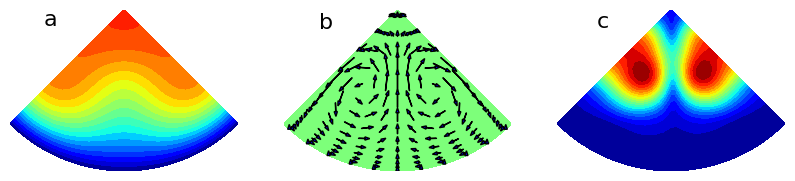
\includegraphics[width=0.9\linewidth]{pipetw_means.png}}
\center{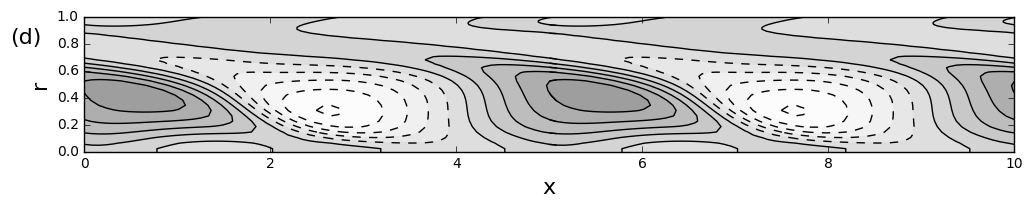
\includegraphics[width=0.9\linewidth]{pipetw_v1_ls.png}}
\caption{Поле скорости бегущей волны, возникающей на сепаратрисе: (a), (b) --- продольная и поперечная компоненты среднего течения $\V_{tw}$, (c) --- амплитуда пульсаций $\v_{n,tw}$, (d) --- продольная компонента пульсаций в сечении $\theta = 0$.}
\label{pipetw_pic}
\end{figure}

Хотя найденная бегущая волна повторяет качественные особенности модельного порыва, наблюдаются существенные количественные отличия. Для сравнения с модельным порывом, на рисунке \ref{pipetw_amp_pic} приведена амплитуда компонент движения бегущей волны, осредненная по времени и по сечению трубы. В отличии от модельного порыва, их значение не зависит от продольной координаты. По аналогии с модельным порывом, в среднем течении $\V_{tw}$ выделена двумерная компонента $\V_{2D,tw} = \overline{\V_{tw}}^\theta$. Трехмерная составляющая движения $\V_{3D,tw} = \V_{tw} - \V_{2D,tw}$ разделена на продольную $\V_{S,tw}$ и поперечную $\V_{V,tw}$, связанные с полосами и продольными вихрями, соответственно. Качественно соотношение между интенсивностью компонент движения сохраняется, однако в модельном порыве они достигают больших значений. Наибольшее отличие демонстрирует поперечное движение $\V_V$, для бегущей волны его значение более, чем в три раза ниже наибольшего значения, достигаемого в модельном порыве. Это может объясняться тем, что решение на сепаратрисе является равновесным. Равновесная интенсивность продольных вихрей в бегущей волне обусловлена необходимостью преодоления диссипирующего влияния вязкости. В модельном порыве необходима большая интенсивность вихрей для того, чтобы не только поддерживать, но и формировать полосы в попадающем внутрь порыва ламинарном течении. 


\begin{figure}
\center{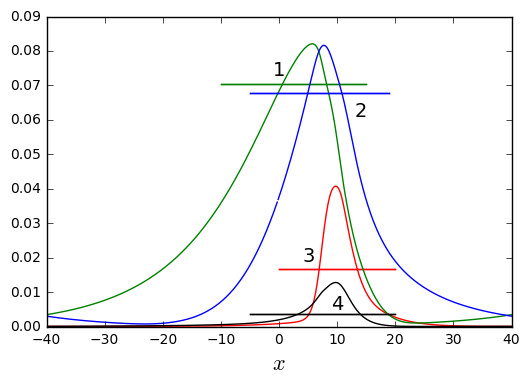
\includegraphics[width=0.5\linewidth]{pipetw_amp.png}}
\caption{Средняя по сечению трубы амплитуда компонент движения бегущей волны (горизонтальные линии) в сравнении с аналогичными величина для модельного порыва (функции переменной $x$): 1 --- движение $\V_S$, ассоциированное с полосами; 2 --- отклонение от течения Пуазейля двумерной компоненты движения $\V_{2D}$; 3 --- пульсационная составляющая движения $\v_n$; 4 --- движение $\V_V$, ассоциированное с продольными вихрями. График повторяет рисунок \ref{amp_pic}.}
\label{pipetw_amp_pic}
\end{figure}

Пульсационная составляющая движения бегущей волны $\v_{n,tw}$ возникает в результате линейной неустойчивости стационарного течения $\V_{tw}$. Наиболее быстро растущее собственное решение линеаризованного уравнения для возмущений \eqref{lin_eq} воспроизводит форму пульсационной составляющей движения и её фазовую скорость. Соответствующий инкремент нарастания $\lambda = 0.0085$. Для сравнения с пульсационной составляющей движения, поле скорости которой представлено на рисунке \ref{pipetw_pic}(c,d), на рисунке \ref{pipetw_lin_pic}(a,b) изображены амплитуда пульсаций, возникающих в линейной задаче, и их мгновенное поле скорости в продольном сечении. Решение линейной задачи имеет более простую форму. Так как среднее течение однородно вдоль трубы и стационарно, линейное решение имеет форму бегущей волны, поле скорости которой меняется по гармоническому закону вдоль трубы и во времени. Как и в случае с модельным порывом, возникающие в рамках линейной задачи пульсации имеют дополнительную симметрию отражения относительно сечения $\theta = \pi/4$, выражаемую уравнением \eqref{dop_sym_eq}. 


\begin{figure}
\center{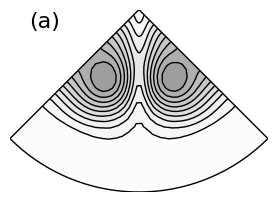
\includegraphics[width=0.3\linewidth]{pipetw_lin_amp.png} 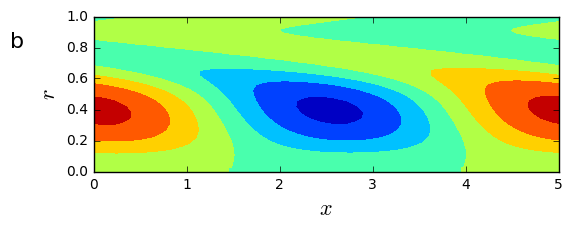
\includegraphics[width=0.6\linewidth]{pipetw_lin_ls.png}}
\caption{Наиболее быстрорастущее собственное возмущение, возникающее на среднем течении $\V_{tw}$: (a) --- амплитуда пульсаций, (b) --- продольная компонента скорости в сечении $\theta = 0$. }
\label{pipetw_lin_pic}
\end{figure}

%\lambda = - 0.0065


Возникающая на сепаратрисе бегущая волна, таким образом, воспроизводит основные элементы цикла самоподдержания модельного порыва, но имеет более простую форму. В сопутствующей системе отсчета её поле скорости оказывается стационарным. В потоке выделяются полосы повышенной и пониженной скорости. Области пониженной скорости имеют зигзагообразную форму. В системе отсчета наблюдателя движение представляет собой периодическое смещение области пониженной скорости в угловом направлении. С периодическим движением может быть ассоциирована пульсационная составляющая поля скорости. Было показано, что она возникает в результате линейной неустойчивости среднего течения, воспроизводящего полосчатый профиль скорости. Среднее течение в этом случае однородно вдоль трубы, что объясняет тот факт, что решение имеет форму бегущей волны. Также в потоке могут быть выделены стационарные продольные вихри, ответственные за образование полосчатого профиля скорости, также не меняющиеся вдоль трубы. Как будет показано далее, простота поведения бегущей волны позволяет выделить некоторые закономерности движения, справедливые также и для модельного порыва, и продемонстрировать их в строго виде. В частности, был выделен механизм нелинейного взаимодействия пульсаций, поддерживающий существование продольных вихрей. 


\section{Механизм образования продольных вихрей на примере точной бегущей волны}

Принято считать, что продольные вихри, ответственные за образование полос, возникают в результате некоторого нелинейного взаимодействия пульсаций, однако его детали не установлены. Прояснить процесс формирования продольных вихрей позволяет анализ уравнения, описывающего эволюцию продольной завихренности, полученного применением оператора Ротора к уравнению Навье-Стокса \eqref{NSeq_cf}:
\begin{equation}\label{ox_eq}
\pd{\omega_x}{t} - \nu\nabla^2 \omega_x =  -  (\v - \c_f, \nabla) \omega_x + (\om, \nabla) v_x
\end{equation}
Здесь $\om = (\omega_x, \omega_r, \omega_\theta) = \rot \v$ --- вектор завихренности, $\c_f$ --- скорость перемещения системы отсчета. Уравнение для стационарной составляющей продольной завихренности получается после осреднения \eqref{ox_eq} вдоль трубы:
\begin{equation}\label{OX_eq}
\pd{\Omega_x}{t} - \nu\nabla^2 \Omega_x = - (\V - \c_f, \nabla) \Omega_x + (\Om, \nabla) V_x - \overline{(\v', \nabla) \omega'_x}^x + \overline{ (\om', \nabla) v'_x }^x
\end{equation}
Здесь  $\Om=(\Omega_x, \Omega_r, \Omega_\theta)$ и $\om'=(\omega'_x, \omega'_r, \omega'_\theta)$ средняя и пульсационная составляющие вектора завихренности. Отметим, что в силу линейности оператора Ротора и осреднения $\Om = \rot \V$, $\om' = \rot \v'$, где $\V$ и $\v'$ --- средняя и пульсационная составляющие поля скорости $\v$. В правой части \eqref{OX_eq} первая пара членов описывает изменение продольной завихренности за счет конвективного переноса и деформации вихревых линий осредненного течения, а вторая пара выражает порождение средней завихренности пульсационным движением. При отсутствии пульсаций продольная завихренность постепенно исчезает под действием вязкости. В рассматриваемом течении система находится в равновесии и стационарная продольная завихренность во времени не меняется. Вязкие диссипация и диффузия компенсируются генерацией завихренности членами в правой части \eqref{OX_eq}.

Для выявления определяющих механизмов генерации средней продольной завихренности удобнее рассмотреть уравнение эволюции квадрата $\Omega_x$, получающееся домножением всех членов \eqref{OX_eq} на $2\Omega_x$. Положительный или отрицательный знак у полученных таким образом выражений в правой части уравнения показывает соответственно положительный или отрицательный вклад этого члена в изменение $\Omega_x^2$, а, следовательно, и в интенсивности поперечного движения. Распределение $\Omega_x^2$ по сечению трубы представлено на рис.~\ref{OXgen_pic}(a). В большей части сечения трубы средняя продольная завихренность близка к нулю. Область концентрации $\Omega_x$ расположена между полосами повышенной и пониженной скорости вблизи области максимальной амплитуды пульсаций.

\begin{figure}
\center{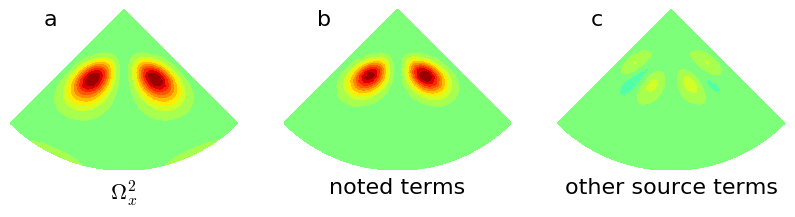
\includegraphics[width=1\linewidth]{pipetw_OXgen.png}}
\caption{Распределение по сечению трубы $\Omega_x^2$ --- (a), вклад в производство $\Omega_x^2$ слагаемых, соответствующих выделенным в \eqref{OXgen_terms} --- (b), вклад остальных слагаемых в правой части \eqref{OX_eq} --- (с). Сплошные линии соответствуют положительным значениям, прерывистые --- отрицательным.}
\label{OXgen_pic}
\end{figure}

При анализе уравнения \eqref{OX_eq} обнаружено, что два слагаемых в правой части вносят определяющий вклад в производство средней продольной завихренности. Они выделены в уравнении ниже:
\begin{equation}\label{OXgen_terms}
\pd{\Omega_x}{t} = - \overline{v'_x \frac{\d \omega'_x}{\d x}}^x + \overline{ \omega'_x \frac{\d v'_x}{\d x} }^x + ... 
\end{equation}
Соответствующее сумме \eqref{OXgen_terms}  распределение в уравнении для $\Omega_x^2$ представлено на рис.~\ref{OXgen_pic}(b), а вклад остальных слагаемых правой части \eqref{OX_eq} показан на рис.~\ref{OXgen_pic}(c). Распределение генерации $\Omega_x^2$ выделенными в \eqref{OXgen_terms} членами практически совпадает по форме с распределением $\Omega_x^2$, тогда как вклад остальных членов не имеет выраженного распределения и на порядок уступает по суммарному вкладу в генерацию $\Omega_x^2$. Таким образом, нет сомнения в том, что стационарные продольные вихри возникают в основном за счет действия выделенной в \eqref{OXgen_terms} пары слагаемых.

Отметим, что пульсации, соответствующие старшей собственной функции линейной задачи об устойчивости среднего стационарного течения, также демонстрируют приведенный выше механизм образования стационарных продольных вихрей. Важно, что это наблюдается только в том случае, когда при анализе устойчивости учитываются как продольная, так и поперечная составляющие среднего течения. Принято считать, что поперечное движение, определяя угловую неоднородность в распределении продольной скорости среднего течения, не может существенным образом влиять на свойства его устойчивости вследствие незначительности своей амплитуды. Поэтому при исследовании линейной устойчивости подобных течений, например, полосчатых структур в турбулентных потоках, наличие поперечного движения обычно не принимается во внимание. В нашем случае пренебрежение поперечным движением приводит к тому, что стационарное течение оказывается линейно устойчивым. Что еще более важно, наименее затухающее возмущение не воспроизводит при этом описанный механизм формирования продольных вихрей. Это связанно с тем, что форма пульсаций продольной завихренности $\omega'_x$ качественно меняется, хотя пульсации продольной скорости $v'_x$ сохраняют свою форму практически неизменной. Тем самым нарушается согласованность  $v'_x$ и $\omega'_x$, необходимая для обеспечения нужного вклада выражения \eqref{OXgen_terms} в производство продольной завихренности.

\begin{figure}
\center{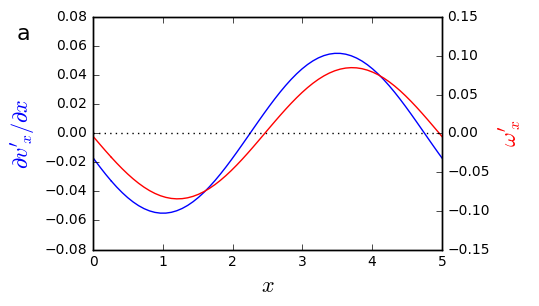
\includegraphics[width=0.5\linewidth]{pipetw_lin_cor.png}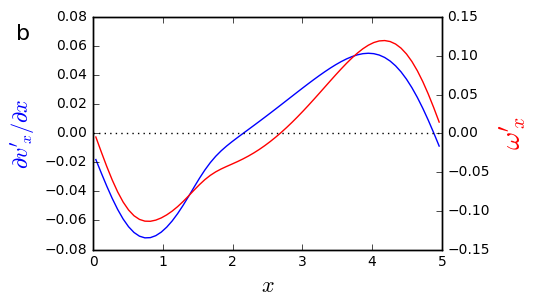
\includegraphics[width=0.5\linewidth]{pipetw_puls_cor.png}}
\caption{Значение $\d v_x' /\d x$ и $\omega_x'$ на прямой, проходящей через область, занятую положительным вихрем, $r = 0.5, \theta = \pi/8$: (a) --- для пульсаций, полученных в линейном приближении; (b) --- для пульсационной составляющей движения $\v_{tw} - \V_{tw}$. }
\label{OXgen_corr_pic}
\end{figure}


Каждое из двух слагаемых в \eqref{OXgen_terms} дает примерно половину общего вклада в производство средней продольной завихренности. Можно показать, что для пульсаций, полученных в рамках линеаризованной постановки, слагаемые \eqref{OXgen_terms} равны друг другу точно. Так как среднее поле скорости $\V_{tw}$ однородно вдоль трубы, возникающие на нем собственные возмущения меняются вдоль трубы по гармоническом закону. При фиксированных значениях $r$ и $\theta$ пусть  $v'_x = a \sin(\alpha x + \phi)$, $\omega_x' = b \sin(\alpha x + \psi)$, тогда:
\begin{equation} \label{OXgen_iterms_1}
 - v'_x \frac{\d \omega'_x}{\d x} = - \alpha a b \sin(\alpha x + \phi) \cos(\alpha x + \psi),
\end{equation}
\begin{equation} \label{OXgen_iterms_2}
\omega'_x \frac{\d v'_x}{\d x} =  \alpha a b \cos(\alpha x + \phi) \sin(\alpha x + \psi),
\end{equation}
\begin{equation} \label{OXgen_iterms_sum}
 - v'_x \frac{\d \omega'_x}{\d x} + \omega'_x \frac{\d v'_x}{\d x} = \alpha a b \sin(\psi - \phi).
\end{equation}
Осредненные вдоль трубы, слагаемые \eqref{OXgen_iterms_1}, \eqref{OXgen_iterms_2} в точности равны друг другу. Более того, сумма \eqref{OXgen_iterms_sum} не зависит от $x$, что, в частности, позволяет упустить знак осреднения вдоль трубы. Эффективность производства  $\Omega_x$ определяется разностью фаз $\psi - \phi$. В области положительного вихря, при $a,b > 0$, наибольшую эффективность как первому, так и второму слагаемому обеспечивает значение $\psi - \phi = \pi/2$. В этом случае $\d v'_x/\d x$ и $\omega'_x$ положительно коррелированы в то время, как $\d v'_x/\d x$ и $\omega'_x$ --- отрицательно. В области отрицательного вихря ситуация меняется на противоположную. Расчет соответствующих коэффициентов корреляции показывает, что они близки к $\pm1$ в соответствующих областях. В качестве подтверждения на рисунке \ref{OXgen_corr_pic}(a) представлены значения $\d v'_x/\d x$ и $\omega'_x$ на прямой, проходящей через область, занятую положительным вихрем, $r = 0.5, \theta = \pi/8$. Фазы выделенных компонент движения практически совпадают. Указанное свойство сохраняется также для пульсационной составляющей движения $\v_{tw} - \V_{tw}$, для которой аналогичные величины изображены на рисунке \ref{OXgen_corr_pic}(b). Объяснить наблюдаемую согласованность фаз позволяет механизм образования пульсаций продольной завихренности, выделенный при исследовании бегущей волны, представленный в следующем разделе. Отметим, что, так как решения являются бегущими волнами, изображенное на рисунке \ref{OXgen_corr_pic} картина течения сохраняется неизменной во времени. 


\section{Механизм образования пульсаций продольной завихренности на примере точной бегущей волны}

Для выявления механизма формирования выделенной связи между пульсациями продольных компонент скорости и завихренности рассмотрим уравнение эволюции $\omega'_x$, получающееся вычитанием \eqref{OX_eq} из \eqref{ox_eq}:
\begin{multline}\label{ox1_eq}
\pd{\omega'_x}{t} - \nu \nabla^2 \omega'_x = - (\V - \c, \nabla) \omega'_x - (\v', \nabla) \Omega_x
+(\Om, \nabla) v'_x + (\om', \nabla) V_x -\\- (\v', \nabla) \omega'_x  + (\om', \nabla) v'_x  + \overline{(\v', \nabla) \omega'_x)}^x  - \overline{(\om', \nabla)}^x
\end{multline}
Работать удобнее с уравнением, описывающим изменение среднего квадрата пульсаций продольной завихренности $\overline{\omega'^2_x}$, получающимся умножением на $2\omega'_x$ каждого из слагаемых в \eqref{ox1_eq} и последующим осреднением вдоль трубы. Слагаемые в этом уравнении не зависят от времени и продольной координаты, сумма слагаемых в правой части балансируется вязким членом в левой части. Как и в предыдущем случае, среди всех слагаемых правой части удается выделить существенные, ответственные за возникновение пульсаций $\omega'_x$.


Распределение $\overline{\omega'_x \omega'_x}^x$ по сечению трубы изображено на рис.~\ref{ox1gen_pic}(a). Основные пульсации $\omega'_x$ наблюдаются в центре расчетной области около оси трубы. На месте расположения продольных вихрей также присутствуют пульсации $\omega'_x$, но меньшей интенсивности. В остальной части трубы их амплитуда близка к нулю. Обнаружено, что за генерацию пульсаций $\omega'_x$ в центральной части трубы и на месте продольных вихрей отвечают два разных механизма. Первый дает пульсации большей амплитуды, однако, за возникновение стационарных продольных вихрей ответственны пульсации, производимые вторым механизмом, так как именно они оказываются согласованными с пульсациями $v'_x$ нужным образом.


\begin{figure}
\center{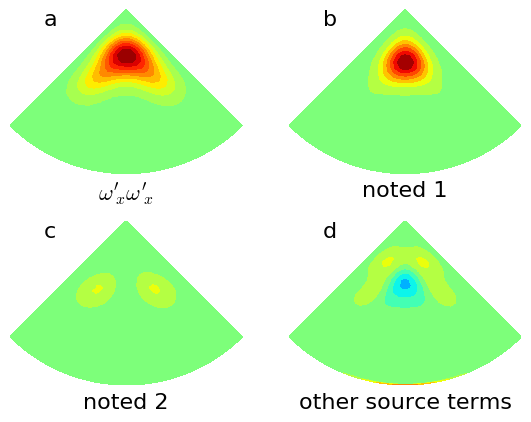
\includegraphics[width=0.66\linewidth]{pipetw_ox1gen.png}}
\caption{Распределение среднего квадрата пульсаций продольной завихренности --- а, вклад в производство $\overline{\omega'_x \omega'_x }^x$ слагаемых \eqref{ox1gen_add_terms} --- (b), слагаемого \eqref{ox1gen_main_terms} --- (c) и суммы остальных слагаемых правой части \eqref{ox1_eq} --- (d).}
\label{ox1gen_pic}
\end{figure}


Первый механизм формирования $\omega'_x$ связан с наличием нормальных к стенке вихрей в пульсационной составляющей движения. Можно провести аналогию между неустойчивостью, возникающей на полосе замедления, и неустойчивостью в следе за телом. Пульсационная составляющая движения напоминает дорожку Кармана. В ней можно выделить последовательность нормальных к стенке вихрей чередующегося знака, двигающихся вниз по полосе пониженной скорости. Им соответствуют области повышенной амплитуды пульсаций радиальной завихренности $\omega'_r$. На рисунке \ref{pipetw_or1_pic} изображена $\omega'_r$ в сечении $r = 0.5$, нормальном к выделенной компоненте завихренности. Приведенные на \ref{pipetw_or1_pic}(a) значения посчитаны по пульсациям, полученным в рамках линеаризованной задачи. Аналогичные значения для пульсационной составляющей движения $\v_{tw} - \V_{tw}$ представлены на рисунке \ref{pipetw_or1_pic}(b). Амплитуда пульсаций продольной завихренности оказывается на порядок ниже амплитуды пульсаций радиальной, угловая завихренность в центральной части трубы также равна нулю в силу симметрии. Таким образом, в центральной части трубы поле завихренности представлено в первую очередь радиальной компонентой и соответствует нормальным к стенке вихрям.

Пульсации продольной завихренности $\omega'_x$ возникают вследствие поворота нормальных к стенке вихрей, происходящего в присутствии градиента продольной скорости $\d V_x/ \d r$, возникающего между полосой замедления и стенкой трубы. Кроме того, наличие радиального градиента $\d V_x/ \d r$ связано с наличием угловой завихренности $\Omega_\theta = \d V_r / \d x - \d V_x / \d r$. Радиальная пульсационная завихренность $\omega'_r = \d v'_x / r \d \theta - \d v'_\theta / \d x$ за счет первого из слагаемых поворачивает стационарные угловые вихри так, что те также приобретают пульсационную продольную составляющую. В уравнении \eqref{ox1_eq} за описанный механизм отвечают слагаемые:
\begin{equation}\label{ox1gen_add_terms}
\frac{\d \omega'_x}{\d t} = \omega'_r \frac {\d V_x}{\d r} + \frac{\Omega_\theta}{r} \frac{\d v'_x}{\d \theta} + ...
\end{equation}
Несмотря на то, что выделенные в \eqref{ox1gen_add_terms} слагаемые имеют противоположные знаки и в значительной степени компенсируют друг друга при сложении, их вклад в производство $\omega'_x$ значителен (смотри рисунок~\ref{ox1gen_pic}(b)). Они определяют форму пульсаций $\omega'_x$ в области между полосой замедления и осью трубы, где пульсации $\omega'_x$ достигают наибольшего значения. Эти пульсации, однако, практически не участвуют в образовании стационарной составляющей продольной завихренности. Это объясняется тем, что колебания $\omega'_x$, рождающиеся в результате описанного механизма, близки по фазе к колебаниям $v'_x$, так что сомножители каждого из слагаемых в выражении \eqref{OXgen_terms} оказываются в противофазе и при осреднении дают близкие к нулю значения.

\begin{figure}
\center{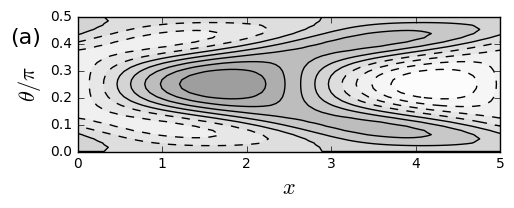
\includegraphics[width=0.45\linewidth]{pipetw_or1_lin.png} 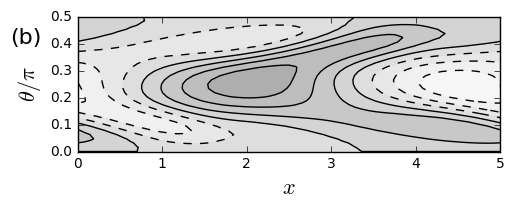
\includegraphics[width=0.45\linewidth]{pipetw_or1.png}}
\caption{Нормальная к стенке компонента завихренности $\omega_r'$ в сечении $r = 0.5$: (а) --- для пульсаций, полученных в рамках линейного приближения; (b) --- для пульсационной составляющей движения $\v_{tw} - \V_{tw}$. }
\label{pipetw_or1_pic}
\end{figure}

Второй механизм образования пульсаций продольной завихренности $\omega'_x$ связан с перераспределением уже существующей стационарной продольной завихренности $\Omega_x$ за счет пульсационной составляющей продольной скорости $v'_x$ (эффект сжатия/растяжения вихревых линий). В уравнении \eqref{ox1_eq} за описываемый механизм отвечает слагаемое
\begin{equation}\label{ox1gen_main_terms}
\frac{\d \omega'_x}{\d t} = \Omega_x \frac {\d v'_x}{\d x} + ...
\end{equation}
Выделенное в \eqref{ox1gen_main_terms} слагаемое стремится произвести пульсации $\omega'_x$, пропорциональные $\d v'_x / \d x$, что обеспечивает наибольшую эффективность образования $\Omega_x$ посредством их нелинейного взаимодействия. Важно, что коэффициентом пропорциональности в \eqref{ox1gen_main_terms} выступает значение средней продольной завихренности, таким образом, механизм включается именно в областях концентрации $\Omega_x$. При этом производимые пульсации $\omega'_x$ положительно пропорциональны пульсациям  $\d v'_x / \d x$ при $\Omega_x>0$ и отрицательно пропорциональны при $\Omega_x<0$, что обеспечивает максимально возможную эффективность производства средней продольной завихренности нужного знака посредством второго из слагаемых выражения \eqref{OXgen_terms}. Очевидно, что пульсации $-v'_x$ и $\d \omega'_x / \d x$ в этом случае также согласованы нужным образом, так что первое слагаемое \eqref{OXgen_terms} близко по значению ко второму.

На рисунке~\ref{ox1gen_pic}(c) приведен вклад выделенного в \eqref{ox1gen_main_terms} слагаемого в производство $\overline{\omega'_x \omega'_x}^x$. Это слагаемое определяет форму пульсаций в области существования продольных вихрей между полосами повышенной и пониженной скорости. Суммарный вклад других слагаемых правой части \eqref{ox1_eq}, не попавших на рис.~\ref{ox1gen_pic}(b,c), изображен на рис.~\ref{ox1gen_pic}(d). Эти слагаемые не имеют существенного значения в процессе генерации $\omega'_x$, их суммарный вклад не превышает нескольких процентов. 

Описанный механизм генерации пульсаций продольной завихренности проявляется в области, где фазовая скорость волны, соответствующей пульсационной составляющей течения, близка по значению к локальной продольной скорости среднего течения. На удалении от точки генерации пульсаций, где фазовая скорость волны существенно отличается от средней скорости, выделенный в \eqref{ox1gen_main_terms} механизм генерации $\omega'_x$ практически не работает. Это объясняется тем, что в системе отсчета, связанной с волной, образующаяся посредством механизма \eqref{ox1gen_main_terms} $\omega'_x$ сносится вдоль трубы средним течением. При этом теряется согласованность фаз между $\d v'_x / \d x$ и $\omega'_x$, что делает её рост невозможным. 


\section{Обобщение полученных при изучении точной бегущей волны результатов на модельный порыв}


\begin{figure}
\center{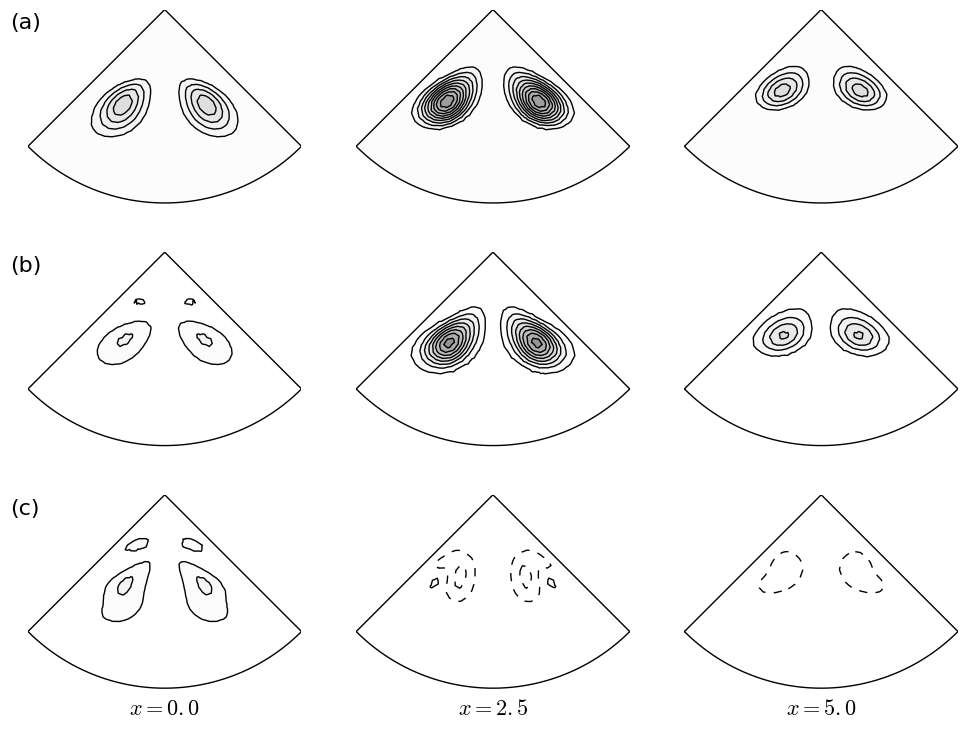
\includegraphics[width=0.9\linewidth]{puff_OXgen.png}}
\caption{В нескольких сечения трубы изображена $\Omega_x^2$ --- в строке (а), а также вклад в образование $\Omega_x^2$ со стороны слагаемых \eqref{OXgen_term} и других слагемых в правой чсти уравнения \eqref{tOX_eq}.}
\label{puff_OXgen_pic}
\end{figure}


Выделенный при изучении бегущей волны, возникающей на сепаратрисе в непротяженной расчетной области, механизм образования продольных вихрей может быть обобщен на модельный порыв. В этом случае осреднение выполняется по времени в системе отсчета, связанной с порывом. Для точной бегущей волны такое осреднение и осреднение вдоль трубы эквивалентны друг другу, так как в системе отсчета порыва она движется. 

Разделим поле завихренности $\om = \rot \v$ на среднюю $\Om = (\Omega_x, \Omega_r, \Omega_\theta) = \overline{\om}^t$ и пульсационную $\om' = (\omega'_x, \omega'_r, \omega'_\theta) = \om - \Om$ составляющие. Как и в случае бегущей волны, поле стационарной продольной завихренности $\Omega_x$ модельного порыва воспроизводит пару продольных вихрей, расположенных по бокам от полосы пониженной скорости. 



Осреднение \eqref{ox_eq} по времени дает уравнение баланса $\Omega_x$: 
\begin{equation} \label{tOX_eq}
\pd{\Omega_x}{t} - \nu\nabla^2 \Omega_x = - (\V - \c_f, \nabla) \Omega_x + (\Om, \nabla) V_x - \overline{(\v', \nabla) \omega'_x}^t + \overline{ (\om', \nabla) v'_x }^t.
\end{equation}

\begin{figure}
\center{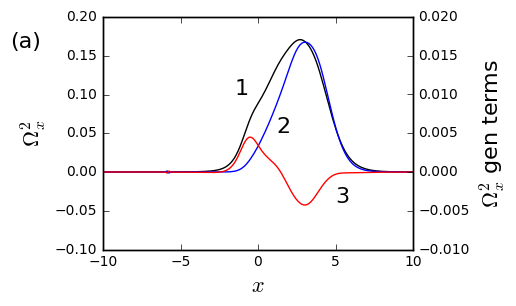
\includegraphics[width=0.5\linewidth]{xline_OXgen.png}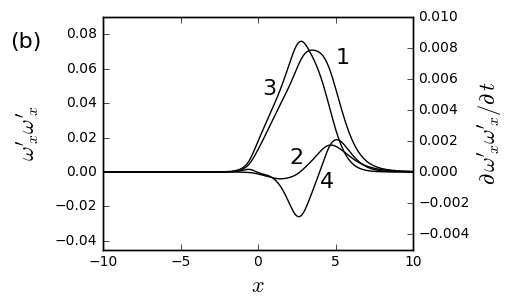
\includegraphics[width=0.5\linewidth]{xline_ox1gen.png}}
\caption{На прямой, проходящей через область, занятую продольным вихрем, при $r = 0.5, \theta = \pi/8$, изображены: (a) --- Квадрат стационарной продольной завихренности (кривая 1) и вклад в его производство со стороны \eqref{OXgen_term} (кривая  2) и других слагаемых в правой части уравнения \eqref{tOX_eq} (кривая  3); (b) --- средний квадрат пульсаций продольной завихренности $\overline{\omega'_x \omega'_x}^t$ (кривая 1) и вклад в его производство со стороны \eqref{ox1gen_term1} (кривая  2), \eqref{ox1gen_term2} (кривая  3) и других слагаемых в правой части уравнения \eqref{tox1gen_eq} (кривая  4).}
\label{xline_oxgen_pic}
\end{figure}


\begin{figure}
\center{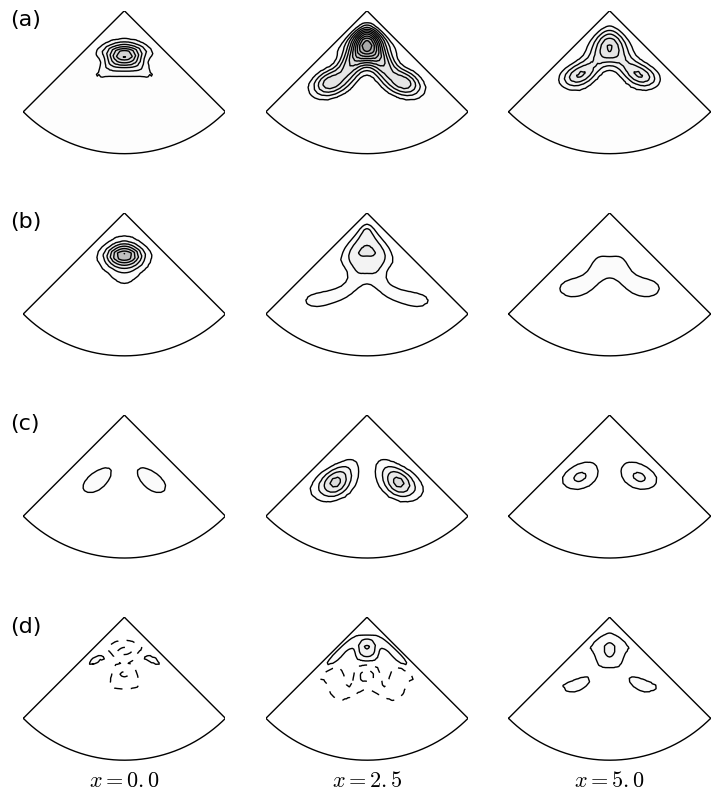
\includegraphics[width=0.9\linewidth]{puff_ox1gen.png}}
\caption{В нескольких сечения трубы изображены: ряд (a) --- интенсивность пульсаций продольной завихренности $\overline{\omega'_x \omega'_x}^t$, ряд (b) --- вклад в образование $\overline{\omega'_x \omega'_x}^t$ со стороны слагаемых \eqref{ox1gen_term1}, ряд (c) --- со стороны слагаемого \eqref{ox1gen_term2}, ряд (d) --- со стороны других других слагаемых в правой части \eqref{tox1gen_eq}. Каждый столбец соответствует одному сечению трубы. }
\label{puff_ox1gen_pic}
\end{figure}

\section{Необходимость учета поперечной компоненты стационарного течения для адекватного воспроизведения формы пульсаций}

Отметим, что пульсации, соответствующие старшей собственной функции линейной задачи об устойчивости среднего стационарного течения, также демонстрируют приведенный выше механизм образования стационарных продольных вихрей. Важно, что это наблюдается только в том случае, когда при анализе устойчивости учитываются как продольная, так и поперечная составляющие среднего течения. Принято считать, что поперечное движение, определяя угловую неоднородность в распределении продольной скорости среднего течения, не может существенным образом влиять на свойства его устойчивости вследствие незначительности своей амплитуды. Поэтому при исследовании линейной устойчивости подобных течений, например, полосчатых структур в турбулентных потоках, наличие поперечного движения обычно не принимается во внимание. В нашем случае пренебрежение поперечным движением приводит к тому, что стационарное течение оказывается линейно устойчивым. Что еще более важно, наименее затухающее возмущение не воспроизводит при этом описанный механизм формирования продольных вихрей. Это связанно с тем, что форма пульсаций продольной завихренности $\omega'_x$ качественно меняется, хотя пульсации продольной скорости $v'_x$ сохраняют свою форму практически неизменной. Тем самым нарушается согласованность  $v'_x$ и $\omega'_x$, необходимая для обеспечения нужного вклада выражения \eqref{OXgen_terms} в производство продольной завихренности.


Описанный механизм генерации пульсаций продольной завихренности объясняет необходимость учета поперечного движения при исследовании устойчивости стационарного течения. Пренебрежение связанной с поперечным движением $\Omega_x$ делает невозможным генерацию $\omega'_x$ в форме, необходимой для сохранения поперечного движения, а следовательно и всего процесса самоподдержания пульсаций.


\section{Выводы по главе}

ы


\chapter{Универсальность полученных результатов}

Представления о механизме поддержания колебаний в течении, описанные в предыдущих главах, получены при изучении только одного решения уравнений Навье-Стокса, найденного при одном числе Рейнольдса. В настоящей главе поднимается вопрос об универсальности полученных результатов. В главе приведены результаты исследования механизма поддержания колебаний в нескольких инвариантных решениях уравнений Навье-Стокса, отличных от модельного порыва. Инвариантными мы называем решения, которые не меняются при переходе к новой системе отчета, отличающейся от исходной некоторым сдвигом во времени и в пространстве. В настоящее время известно достаточно большое число различных инвариантных решений уравнений Навье-Стокса \cite{Kawahara2012}. Наиболее простым примером трехмерных инварианты решений являются бегущие волны. Их поле скорости периодично вдоль потока и стационарно в подходящей подвижной системе отсчета. Более сложным примером являются условно периодические решения, то есть решения, являющиеся в подходящей подвижной системе отсчета периодическими по времени. Частным случаем условно периодического решения является модельный порыв. По аналогии с модельным порывом, может быть выполнено детальное исследование таких решений. 


Опираясь на модельный порыв методом продолжения по параметру в работе найдено семейство условно периодических решений уравнений Навье-Стокса с пространственно локализованной структурой. В соответствии с \cite{Avila2013}, среди найденных таким образом решений существуют решения, по ряду качественных характеристик оказывающиеся ближе к турбулентному порыву, чем модельный порыв.  Также в работе было найдено несколько семейств решений уравнений Навье-Стокса, имеющих вид бегущей волны, описывающих движение жидкости в круглой трубе и в плоском канале. Описаны основные характеристик найденных решений и механизм поддержания колебаний в них. Во всех исследованных решениях основные элементы механизма поддержания колебаний оказываются такими же, как и в модельном порыве, что в некоторой степени говорит об их универсальности. В главе дано описание метода Ньютона-Крылова, позволяющего находить условно периодические решения уравнений Навье-Стокса, а также решения, имеющие вид бегущей волны, как частный случай условно периодических решений. Дано описание метода продолжения по параметру, опирающегося на метод Ньютона-Крылова. Представлены результаты анализа полученных решений. Анализ решений в виде бегущей волны, описывающих движение жидкости в плоском канале, опубликован в работах автора \cite{Vest18, KMU16}. 

\section{Метод Ньютона-Крылова для поиска условно периодических решений уравнений Навье-Стокса}

Условно периодическим мы называем решение уравнений Навье-Стокса, являющееся периодическим по времени в подходящей подвижной системе отсчета. В работе реализован метод Ньютона-Крылова \cite{Sanchez2004, Viswanath2007, Dijkstra2014}, позволяющий численно находить мгновенные поля скорости, соответствующие условно периодическим решениям. Мгновенное поле скорости  $\v_\mathrm{p}(x,r,\theta)$ соответствует условно периодическому решению, если интегрирование уравнений движения с $\v_\mathrm{p}$ в качестве начальных данных в течении времени $T_\mathrm{p}$ в системе отсчета, перемещающейся со скоростью $c_\mathrm{p}$, дает поле скорости, совпадающее с $\v_\mathrm{p}$:
\begin{equation}\label{P_eq}
\phi(\v_\mathrm{p}, T_\mathrm{p}, c_\mathrm{p}, \Re) = \v_\mathrm{p}.
\end{equation}
В этом случае $T_\mathrm{p}$  --- временной период решения, $c_\mathrm{p}$ --- скорость перемещения решения вдоль трубы. Функция $\phi(\v, t, c, \Re)$ имеет значение поля скорости, полученного интегрированием уравнений движения c начальным полем скорости $\v$ в течении времени $t$ в системе отсчета, перемещающейся со скоростью $c$, при числе Рейнольдса $\Re$. Заметим, что при условии несжимаемости давление в каждый момент времени с точностью до константы определяется по мгновенному полю скорости, что позволяет исключить давление из \eqref{P_eq} и других уравнений. 

Если $\v_1(x,r,\theta)$ --- решение \eqref{P_eq}, то $\v_2(x, r, \theta) = \v_1(x + \Delta x, r, \theta)$ и $\v_3 = \phi(\v_1, \Delta t, c, \Re)$ при произвольных $\Delta x$ и $\Delta t$ также являются решениями \eqref{P_eq}, соответствующими одному условно периодическому решению уравнений Навье-Стокса. Для того, чтобы с каждым условно периодическим решением связать только одно поле скорости $\v_\mathrm{p}$, на решения уравнения \eqref{P_eq} накладываются два дополнительных условия, фиксирующих положение решения во времени и в пространстве:
\begin{equation} \label{P1_eq}
\pd{}{t} \big|\big| \phi(\v_\mathrm{p}, t, c, \Re) - \v_\mathrm{Pois} \big|\big|_\mathrm{3D} \Big|_{t=0} = 0,
\end{equation}
\begin{equation} \label{P2_eq}
\pd{}{x} \big|\big| \v_\mathrm{p} - \v_\mathrm{Pois} \big|\big|_\mathrm{2D} \Big|_{x = 0} = 0. 
\end{equation}
В условии \eqref{P1_eq} вычисляется среднее по объему трубы отклонение решения от течения Пуазейля $\v_{\mathrm{Pois}}$ в два близких к нулю момента времени и требуется, чтобы их разность была равна нулю. В \eqref{P2_eq} требуется равенство нулю разности средних отклонений решения от течения Пуазейля в двух близких к $x=0$ поперечных сечениях трубы (в начальный момент времени). Значение $c$ в \eqref{P1_eq} может быть произвольным и на результат не влияет. 


Нелинейное уравнение \eqref{P_eq} с двумя дополнительными условиями решается численно методом Ньютона. Метод Ньютона итерационный и на каждом шаге позволяет уточнить существующее приближение к решению. Для системы $F(x) = 0$ метод Ньютона формулируется следующим образом. Пусть $x_m$ --- приближение к решению на шаге $m$, $x^*$ --- точное решение. Разложение $F(x^*)$ в ряд около точки $x_m$ имеет вид:
\begin{equation}
F(x^*) = F(x_m) + \pd{F}{x}\bigg|_{x=x_m} \Delta x_m^* + O(\Delta x_m^{*2}), 
\end{equation}
где $\Delta x_m^* = x^* - x_m$. Пренебрегая нелинейными относительно $\Delta x_m^*$ слагаемыми, учитывая, что $F(x^*) = 0$, получим линейную систему на поправку к решению:
\begin{equation}\label{Newton_eq}
J \Delta x_m = b,
\end{equation}
где $J$ --- матрица Якоби:
$$
J = \frac{\partial F}{\partial x}\bigg|_{x = x_m},
$$
вектор $b = - F(x_m)$. 
Основной задачей при применении метода Ньютона является решение линейной системы \eqref{Newton_eq}. Новое приближение к решению вычисляется по формуле: 
\begin{equation} \label{end_NK_eq}
x_{m+1} = x_m + \Delta x_m. 
\end{equation}

Для решения линейной системы \eqref{Newton_eq} применяется итерационный алгоритм, в котором приближение к решению находится в подпространствах Крылова $K_i = span\{b, Jb, J^2b, ... , J^ib\}$, где $span\{a_1, ..., a_i\}$ обозначает линейную оболочку векторов $a_1, ..., a_i$. Построение базиса в подпространстве $K_{i+1}$ при условии, что базис в подпространстве $K_i$ уже известен, требует одного умножение уже известного вектора $J^ib$ на $J$ ($K_0 = span\{b\}$). Произведение матрицы Якоби $J$ на вектор единичной длины $e$ равно производной от функции $F$ в соответствующем направлении:
\begin{equation} \label{Je_eq}
Je = \pd{F}{x} e = \pd{F}{e}. 
\end{equation}
Таким образом, построение базиса в подпространствах Крылова сводится к вычислению производных по направлению от функции $F$. Значение производной функции $F$ по направлению $e$ приближается конечной разностью, которая может быть найдена численно:
\begin{equation}\label{fd_eq}
\pd{F}{e} \approx \frac{F(x + \varepsilon e) - F(x)}{\varepsilon}.
\end{equation}
В наших расчетах действительные числа представляются 64-битными числами с плавающей запятой. В этом случае значение $\varepsilon$ рекомендуется выбирать близким к $10^{-7}$ \cite{Viswanath2007}. Метод Ньютона, в котором приближения к решениям системы \eqref{Newton_eq} находятся в подпространствах Крылова, называют также методом Ньютона-Крылова \cite{Sanchez2004}. 

В работе для решения линейной системы \eqref{Newton_eq} применяется метод минимизации невязки \cite{EEbook}. Этот метод также итерационный. На $i$-ом шаге выполнения метода в подпространстве Крылова $K_i$ ищется приближение к решению $x_i$ таким образом, что невязка $r_i = b - Ax_i$ имеет наименьшую длину. Критерием остановки итерационного процесса служит снижение длины невязки ниже заранее заданной величины, либо превышение заранее заданного числа итераций. При поиске условно периодических решений с небольшим числом неустойчивых направлений (менее 10), для уточнения решения на порядок требуется несколько десятков итераций метода минимизации невязки, причем число итераций  практически не зависит от параметров расчетной сетки (при условии, что сетка достаточно подробна для адекватного воспроизведения решения) \cite{Dijkstra2014}. На каждой итерации метода минимизации невязки требуется однократно вычислить значение функции $F$ в новой точке. В нашем случае вычисление функции $F$ связано с численным интегрированием уравнений движения в течении времени $T_p$, что требует значительных вычислительных ресурсов. Сравнительно небольшое число обращений к функции $F$ делает реализованный метод Ньютона-Крылова эффективным инструментом поиска условно периодических решений, имеющих небольшое число неустойчивых направлений.

Для построения подпространств Крылова необходимо, чтобы матрица $J$ была квадратной. Если поле скорости задается $N$ параметрами, то в матрице $N+2$ строки. Соответственно, вместе с полем скорости в число неизвестных необходимо включить два параметра системы, например, временной период $T_p$ и скорость системы отсчета $c_p$. Тогда свободным параметром остается только число Рейнольдса $\Re$. $T_p$ и $c_p$ играют роль собственных значений системы, при которых условно периодическое решение существует. 

Критерием остановки итерационного процесса метода Ньютона может служить снижение нормы невязки ниже заранее заданной величины, либо превышение заранее заданного числа итераций. 


%Невязка имеет наименьшую длину, если она перпендикулярна пространству $AK_i$. Проще всего опустить перпендикуляр из вектора $b$ на подпространство $AK_i$, имея в этом подпространстве ортогональный базис. Построим последовательность векторов $q_1, \dots, q_i$ таким образом, что они образуют базис в подпространстве $K_i$, а вектора $p_1 = Aq_1, \dots, p_i = Aq_i$ образуют ортогональный базис в подпространстве $AK_i$. Тогда легко может быть построено ортоганальное разложение правой части уравнения вида $b = \alpha_1 p_1 + \dots + \alpha_i p_i + r_i$, где $b_i =  \alpha_1 p_1 + \dots + \alpha_i p_i$ лежит в пространстве $AK_i$, а $r_i$ перпендикулярно ему. Коэффициенты разложения дает формула:
%\begin{equation}
%\alpha_k = (b,p_k) / (p_k, p_k),
%\end{equation}
%где $(\ ,\ )$ ---  скалярное произведение, порождающее норму, в которой минимизируется невязка. 
%Так как у каждого вектора $p_k$ известен прообраз $q_k$, линейная комбинация векторов $q_k$ с коэффициентами $\alpha_k$ дает приближение к решению, лежащее в пространстве $K_i$
%\begin{equation}
%\x_i = \alpha_1 q_i + \dots + \alpha_i q_i. 
%\end{equation}
%Переход на $i+1$ итерацию алгоритма связан с построением базиса подпространств $K_{i+1}$ и $AK_{i+1}$. Для построения ортогонального базиса в подпространстве $AK_{i+1}$ базис подпространства $AK_i$ пополняется новым вектором $p_{i+1}$, полученным ортогонализацией с уже известными базисными векторами $p_1, \dots, p_i$ вектора $Ap_i$. В процессе ортогонализации также может быть получен вектор $q_{i+1}$, являющийся прообразом вектора $p_{i+1}$. 

%Критерием остановки итерационного процесса при решении линейной системы может служить снижение величины невязки ниже заранее заданного порогового значения, либо превышение заранее заданного числа итераций. Переход на новый шаг выполнения метода требует однократного вычисления произведения матрицы $A$ на вектор, связанного с вычисление производной функции $F$ вдоль одного направления в соответствии с \eqref{Jl_eq}, \eqref{fd_eq}. В процессе вычислений необходимо хранить две последовательности векторов $p_1, \dots, p_i$ и $q_1, \dots, q_i$. На первой итерации $q_1 = b$, $p_1 = Ab$.  


\section{Продолжение модельного порыва по числу Рейнольдса} \label{contin_sec}

Основной сложностью при нахождении новых условно периодических решений оказывается подбор подходящего начального приближения к решению, с которым метод Ньютона сойдется. Однако если одно условно периодическое решение известно, оно может быть использовано в качестве начального приближения для решения с близкими значениями параметров. Найденное решение, в свою очередь, также может выступать в качестве начального приближения к новому решению при близком значении параметров. Таким образом, может быть построена цепочка решений, связывающая решения с существенно различным значением параметров. Такой метод нахождения новых решений называют методом продолжения по параметру \cite{Viswanath2007, Dijkstra2014}. Для построения приближения к новому решению при условии, что известно уже два или более решений при близких значениях параметров, в работе применялась линейная интерполяция. Такой подход позволяет существенно (приблизительно в 10 раз) увеличить допустимый шаг, с которым выполняется продвижение по параметру от одного решения в другому. 

Продолжая решение, соответствующее модельному порыву, по числу Рейнольдса, удалось получить новые условно периодические решения с пространственно локализованной структурой. На рисунке \ref{local_contin_pic} представлены значения $T_p$, $c_p$ и $\Re$ для найденных таким образом решений. Как показывают расчеты, решения принадлежат однопараметрическому множеству, что согласуется с \cite{Avila2013}. Решения, принадлежащие различным кривым, найдены на различных расчетных сетках. Параметры сеток, на которых выполнены расчеты, приведены в разделе \ref{edge_seq}. Черная точка на каждом из графиков соответствует исходному решению --- модельному порыву. При $\Re = \Re^* = 1400$ обнаружена точка бифуркации, в которой порождаемое модельным порывом семейство решений рождается (в \cite{Avila2013} сообщается о $\Re^* = 1430$). При меньших значениях числа Рейнольдса решений не существует. При больших значениях числа Рейнольдса существует две ветви решений, то есть при каждом значении $\Re$ существует два решения, каждое из которых принадлежит свой ветви. Исходное решение принадлежит нижней ветви (на графиках она оказывается выше). Для решений с нижней ветви характерна меньшая амплитуда колебаний, меньшая интенсивность поперечного движения и большие значения $T_p$ и $c_p$. Для того, чтобы в точке бифуркации перейти с нижней ветви решений на верхнюю, $\Re$ было включено в число определяемых параметров, а продолжение решения было выполнено по $T_p$ или $c_p$. Для того, чтобы адекватно воспроизвести решения с верхней ветви, необходимы более подробные расчетные сетки. Характеристики решений с верхней ветви, полученные на различных сетках, согласуются между собой до $\Re \approx 1700$. При больших $\Re$ между решениями, полученными на различных сетках, начинают проявляться некоторые качественные отличия. Для более подробного анализа верхней ветви выбрано решение с $\Re = 1700$. Мы полагаем, что используемые нами расчетные сетки позволяют адекватно воспроизвести это решение. 


\begin{figure}
\center{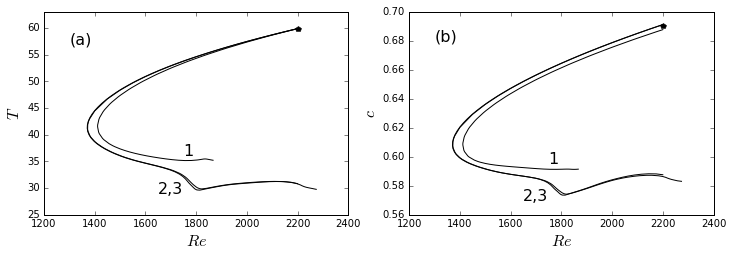
\includegraphics[width=0.9\linewidth]{local_contin.png}}
\caption{Продолжение решения, соответствующего модельному порыву, по числу Рейнольдса: (а) зависимость временного периода $T$ и (b) скорости перемещения порыва вдоль трубы $c$ от числа Рейнольдса $\Re$. Кривые 1, 2 и 3 соответствуют решениям, полученным на различных расчетных сетках. Черные точки соответствует исходному решению, принадлежащему сепаратрисе.}
\label{local_contin_pic}
\end{figure}

Решения с верхней ветви сохраняют пространственно локализованную структуру, но в сравнении с решениями с нижней ветви, имеют большую амплитуду колебаний, большую интенсивность поперечного движения, больший дефект скорости на оси трубы. Скорость перемещения локализованной структуры вдоль трубы для решений, принадлежащих верхней ветви, оказывается ниже, чем для решения, принадлежащих нижней ветви. По всем этим параметрам решения, принадлежащие верхней ветви, оказываются ближе к турбулентному порыву, чем решения, принадлежащие нижней ветви. Это дает основания полагать, что и другие результаты, полученные при изучении решений, принадлежащих верхней ветви, также имеют большее отношение к турбулентному порыву. В решении, принадлежащем верхней ветви, $\Re = 1700$, скорость перемещения локализованной структуры вдоль трубы составляется $0.59U$. Скорость перемещения локализованной структуры в исходном решении, принадлежащем нижней ветви, (модельном порыва) составляет $0.69U$. Скорость перемещения турбулентного порыва приблизительно равна $0.5U$. Временной период решения, принадлежащего верхней ветви, $\Re = 1700$, составляет $34.4 R/U$, что почти в два раза меньше, чем в модельном порыве ($59.6R/U$). 

\section{Исследование верхней ветви порожденного модельным порывом семейства решений}

\begin{figure}
\center{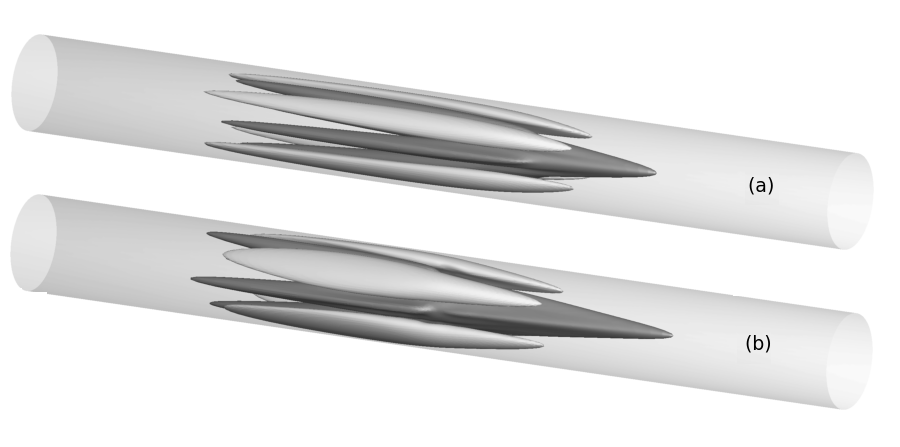
\includegraphics[width=0.9\linewidth]{3D_contin_cmp.png}}
\caption{Среднее поле скорости исходного решения (a) и решения, принадлежащего верхней ветви, $\Re=1700$, (b). Темным и светлым тоном приведены поверхности скорости $-0.1$ и $+0.1$ относительно скорости течения Пуазейля. Поток направлен слева направо.}
\label{3D_contin_cmp_pic}
\end{figure}

Также, как при исследовании модельного порыва, полученного на сепаратрисе, поле скорости $\v_\mathrm{ub}$ модельного порыва, принадлежащего верхней ветви, $\Re = 1700$, представляется в виде суммы средней $\V_\mathrm{ub} = \overline{\v_\mathrm{ub}}^t$ и пульсационной $\v_\mathrm{n,ub} = \v_\mathrm{ub} - \V_\mathrm{ub}$ составляющих; осреднение выполняется по времени в сопутствующей системе отсчета (<<ub>> --- <<up branch>>). Среднее поле скорости $\V_\mathrm{ub}$ представлено на рисунке \ref{3D_contin_cmp_pic} (b). На рисунке (a) для сравнения представлено среднее поле скорости исходного решения. Качественно структура решения не меняется, среднее поле скорости в обоих случаях содержит полосы повышенной и пониженной скорости, вытянутые вдоль стенки. Полосы пониженной скорости объединяются в передней части порыва в приосевой области, формируя центральное ядро пониженной скорости. В случае решения с верхней ветви ядро пониженной скорости имеет большую протяженность, в то время как пристенные полосы оказываются короче. Суммарная длина структуры при этом практически не меняется. 


\begin{figure}
\center{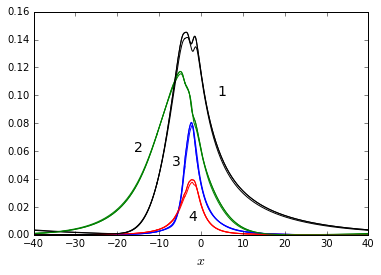
\includegraphics[width=0.6\linewidth]{amp_ub.png}}
\caption{Распределение вдоль трубы амплитуды компонент решения, принадлежащего верхней ветви, $\Re = 1700$: кривая 1 --- $\V_\mathrm{2D,ub}$ (отклонение от течения Пуазейля), кривые 2,4 --- продольная а поперечная компоненты $\V_\mathrm{3D,ub}$, кривая 3 --- амплитуда $\v_\mathrm{n,ub}$. Представлены результаты, полученных на трех расчетных сетках, описанных в разделе \ref{edge_seq}.}
\label{amp_ub_pic}
\end{figure}


На рисунке \ref{amp_ub_pic} изображена средняя по сечению трубы амплитуда различных компонент движения. Как при исследовании модельного порыва, стационарная составляющая движения разделена на двумерную $\V_\mathrm{2D,ub} = \overline{\V_\mathrm{ub}}^{\theta}$ и трехмерную $\V_\mathrm{3D,ub} = \V_\mathrm{ub} - \V_\mathrm{2D,ub}$ составляющие. Продольная и поперечная компоненты трехмерной составляющей движения ассоциируются с полосами и продольными вихрями, соответственно. Качественно, распределение интенсивности различных компонент движения вдоль трубы в рассматриваемом решении, принадлежащем верхней ветви, и в модельном порыве совпадают (см. рис. \ref{amp_pic}), но все компоненты движения в решении, принадлежащем верхней ветви, имеют большую амплитуду. Амплитуда полосчатого движения и пульсаций выше примерно в два раза. Интенсивность продольных вихрей выше почти в четыре раза. На рисунке \ref{amp_ub_pic} представлены результаты, полученные на трех различных расчетных сетках. Параметры расчетных сеток приведены в разделе \ref{edge_seq}. Результаты, полученные на различных сетках, совпадают качественно и близки количественно, что позволяет говорить об адекватности воспроизведения решения в расчетах. 


\begin{figure}
\center{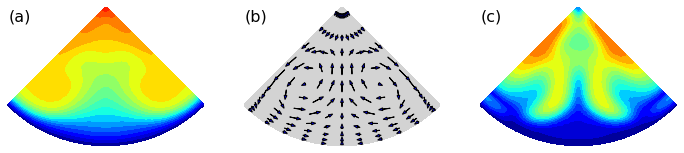
\includegraphics[width=0.9\linewidth]{local_ub_means.png}} 
\center{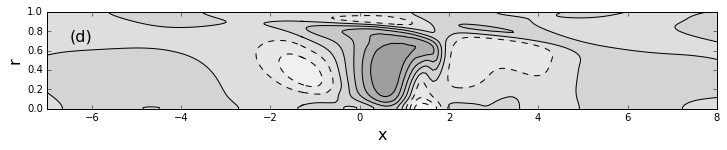
\includegraphics[width=0.9\linewidth]{local_ub_vel1.png}}
\caption{Поле скорости решения, принадлежащего верхней ветви, $\Re = 1700$: в сечении, где пульсации достигают наибольшей амплитуды, приведены изолинии $V_\mathrm{x,ub}$ (a), векторное поле $(V_\mathrm{r,ub}, V_\mathrm{\theta,ub})$ (b), линии равного уровня амплитуды $\v_\mathrm{n,ub}$ (c); в сечении $\theta = 0$ --- изолинии продольной компоненты $\v_\mathrm{n,ub}$ (d). Сплошные линии --- положительные значения, прерывистые --- отрицательные.}
\label{local_ub_means_pic}
\end{figure}

На рисунке \ref{local_ub_means_pic}(a) приведена продольная компонента стационарной составляющей движения $V_\mathrm{x,ub}$ в сечении трубы, где пульсации достигают максимума. В сравнении с исходным решением в решении, принадлежащем верхней ветви, между полосами повышенной и пониженной скорости существуют области, в которых продольная скорость с ростом $r$ (при постоянных $x$ и $\theta$) падает не монотонно. Полосы формируются за счет <<лифт-ап>> эффекта. Векторное поле поперечной компоненты среднего течения $(V_\mathrm{r,ub}, V_\mathrm{\theta,ub})$, приведенное на рисунке (b), соответствует наличию стационарных продольных вихрей между полосами повышенной и пониженной скорости, ответственных за поддержание существования этих полос. На рисунке (с) приведена амплитуда пульсационной составляющей движения $\v_\mathrm{n,ub}$. Пульсации в решении, принадлежащем верхней ветви, имеют более сложную форму, чем в исходном решении, но они также оказываются сконцентрированы между полосой повышенной скорости и осью трубы и между соседними полосами повышенной и пониженной скорости. Форма пульсационной составляющей движения близка к бегущей волне, имеющей в системе отсчета порыва положительную фазовую скорость. Также, как и в модельном порыве, длину этой бегущей волны можно оценить в $5R$. Мгновенное поле скорости пульсационной составляющей движения в продольном сечении трубы $\theta = 0$ приведено на рисунке~(d).  


\begin{figure}
\center{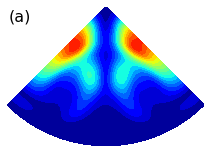
\includegraphics[width=0.3\linewidth]{ub_lin_cs.png} 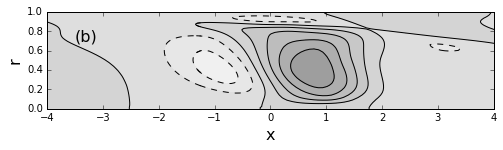
\includegraphics[width=0.6\linewidth]{ub_lin_ls.png}}
\caption{Наиболее быстрорастущее решение линейной задачи устойчивости поля скорости $\V_\mathrm{ub}$:  (а) --- линии уровня амплитуды колебаний в поперечном сечении трубы, где амплитуда колебаний достигает максимума, (b) --- мгновенное поле скорости в сечении $\theta = 0$. Сплошные линии --- положительные значения, прерывистые --- отрицательные.}
\label{ub_lin_pic}
\end{figure}

Также, как в модельном порыве, в решении, принадлежащем верхней ветви, $\Re = 1700$, среднее поле скорости оказывается линейной неустойчиво. Наиболее быстрорастущее решение $\v'_\mathrm{1,ub}$ линейной задачи устойчивости поля скорости $\V_\mathrm{ub}$ воспроизводит форму пульсационной составляющей движения $\v_\mathrm{n,ub}$ и период её изменения во времени, что говорит о том, что пульсационная составляющая движения $\v_\mathrm{n,ub}$ возникает в результате линейной неустойчивости среднего течения. Временной период и инкремент нарастания $\v'_\mathrm{1,ub}$ равны $31.8R/U$ и $0.012U/R$. Временной период $\v_\mathrm{n,ub}$ равен $34.4R/U$. На рисунке \ref{ub_lin_pic}(a) в том же сечении, в котором пульсационная составляющая движения представлена на рисунке \ref{local_ub_means_pic}(c), приведена средняя по времени амплитуда колебаний в решении $\v'_\mathrm{1,ub}$. Распределение амплитуды колебаний для решения линеаризованных и решения полных уравнений достаточно точно совпадают. В $\v'_\mathrm{1,ub}$ колебания также оказываются сконцентрированы между полосой повышенной скорости и осью трубы и между соседними полосами повышенной и пониженной скорости. Мгновенное поле продольной компоненты $\v'_\mathrm{1,ub}$, представленное в продольном сечении $\theta = 0$ на рисунке \ref{ub_lin_pic}(b), также демонстрирует согласие с мгновенным полем скорости $\v_\mathrm{n,ub}$, приведенным на рисунке \ref{local_ub_means_pic}(d). В области расположения полосы повышенной скорости вдоль потока друг за другим следуют области повышенной и пониженной скорости. Суммарная протяженность одной области повышенной скорости и одной области пониженной скорости составляет приблизительно $5R$. Общая протяженность области, в которой пульсации имеют существенную амплитуду, равна примерно $5$--$7R$. По форме пульсации близки к бегущей волне, что согласуется с тем, что они возникают в результате линейной неустойчивости среднего течения, слабо меняющегося вдоль трубы. Отметим, что поле скорости $(V_\mathrm{x,ub}, 0, 0)$ оказывается линейно устойчивым, соответствующий инкремент затухания равен $\lambda = -0.009U/R$. 


\begin{figure}
\center{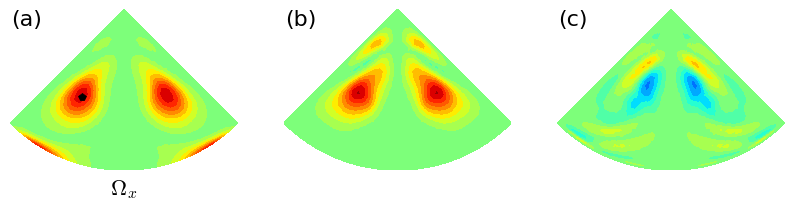
\includegraphics[width=0.9\linewidth]{ub_OXgen_map.png}}
\caption{Механизм поддержания стационарных продольных вихрей в условно периодическом решении, принадлежащем верхней ветви, $\Re = 1700$. В сечении трубы, где пульсации достигают наибольшей амплитуды, приведены линии уровня: (a) --- $\Omega_x^2$, (b) и (c) --- вклад в поддержание $\Omega_x^2$ со стороны слагаемых \eqref{time_OXgen_terms} и суммы других слагаемых в правой части уравнения \eqref{time_OX_eq}. Сплошные линии соответствуют положительным значения, прерывистые --- отрицательным.}
\label{ub_OXgen_pic}
\end{figure}


Механизмы поддержания стационарных продольных вихрей в решении, принадлежащем верхней ветви, и в модельном порыве также согласуются. На рисунке \ref{ub_OXgen_pic}(a) приведен квадрат стационарной продольной завихренности $\Omega_\mathrm{x, ub}^2$ в сечении трубы, где амплитуда пульсаций достигает наибольшей величины. Распределение $\Omega_\mathrm{x,ub}^2$ по сечению трубы соответствует наличию пары продольных вихрей, расположенных между полосами повышенной и пониженной скорости (см. рис. \ref{local_ub_means_pic}(b)). На рисунках \ref{ub_OXgen_pic}(b,c) приведены значения слагаемых \eqref{time_OXgen_terms} и других слагаемых из правой части уравнения \eqref{time_OX1_eq}, умноженные на $2\Omega_\mathrm{x,ub}$. Умножение слагаемых из правой части уравнения \eqref{time_OX1_eq} на $2\Omega_\mathrm{x,ub}$ дает вклад этих слагаемых в поддержания поля $\Omega_\mathrm{x,ub}^2$. Слагаемые \eqref{time_OXgen_terms} определяют форм поля стациоанрной продольной завихренности, вклад других слагаемых в правой части \eqref{time_OX1_eq} оказывается отрицательным. Нет сомнения, что за образование стационарных продольных вихрей в уравнении \eqref{time_OX1_eq} ответственны слагаемые \eqref{time_OXgen_terms}. Дополнительно, на рисунке \ref{ub_oxgen_lines_pic}(a) приведено значение $\Omega_x^2$ и слагаемых, отвечающих за его формирование, на прямой, проходящей через область, занятую положительным вихрем, $r = 0.6, \theta = \pi/10$. Картина течения в этом случае значительно сложнее, чем в модельном порыве (см. рис. \ref{xline_oxgen_pic}(a)). Тем не менее, графики на рисунке \ref{ub_oxgen_lines_pic}(a) также подтверждают представление о том, что за образование продольных вихрей ответственно слагаемое \eqref{time_OXgen_terms}. 
 

\begin{figure}
\center{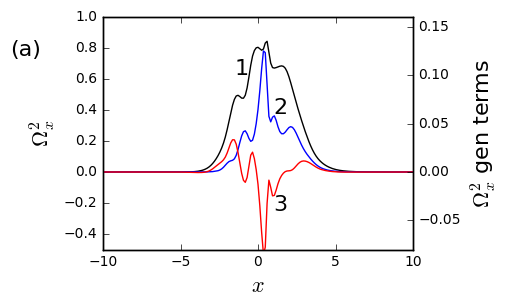
\includegraphics[width=0.5\linewidth]{ub_OXgen_lines.png}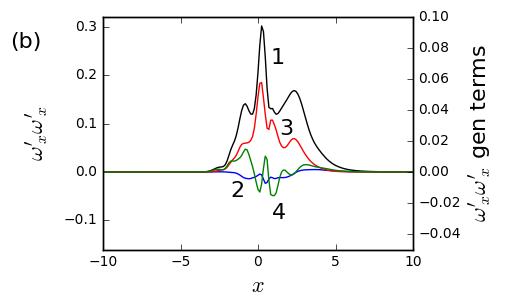
\includegraphics[width=0.5\linewidth]{ub_ox1gen_lines.png}}
\caption{Механизм поддержания продольных вихрей в условно периодическом решении, принадлежащем верхней ветви, $\Re = 1700$. На прямой, проходящей через область, занятую положительным вихрем, $r = 0.6$, $\theta = \pi/10$, приведены значения: (a) --- $\Omega_x^2$ (кривая 1) и вклад в его поддержание со стороны слагаемых \eqref{time_OXgen_terms} (кривая 2) и других слагаемых в правой части \eqref{time_OX1_eq} (кривая 3); (b) --- $\overline{\omega'_x\omega'_x}^t$ (кривая 1) и вклад в её поддержание со стороны слагаемого \eqref{time_ox1gen_term2} (кривая 2) и других слагаемых в правой части уравнения \eqref{time_ox1_eq} (кривая~3).} 
\label{ub_oxgen_lines_pic}
\end{figure}


То, что слагаемые \eqref{time_OXgen_terms} не равны нулю, говорит о наличии согласованности между пульсациями продольной скорости и пульсациями продольной завихренности. Объяснить наличие согласованности позволяет механизм образования пульсаций продольной завихренности, выделенный в рассматриваемом решении. Механизмы образования пульсаций продольной завихренности в рассматриваемом решении и в модельном порыве также согласуются. В уравнении \eqref{time_ox2_eq}, описывающем эволюцию пульсаций продольной завихренности $\omega'_\mathrm{x,ub}$, за образование $\omega'_\mathrm{x,ub}$ в области расположения продольных вихрей отвечает слагаемое \eqref{time_ox1gen_term2}. На рисунке \ref{ub_oxgen_lines_pic}(b) также, как на рисунке (a), приведено значение амплитуды пульсационной составляющей движения $\overline{\omega'_\mathrm{x,ub}\omega'_\mathrm{x,ub}}^t$ и вкладов в её образование со стороны слагаемых \eqref{time_ox1gen_term2} и других слагаемых в правой части уравнения \eqref{time_ox2_eq}. Вклад слагаемых уравнения \eqref{time_ox2_eq} в поддержание $\overline{\omega'_\mathrm{x,ub}\omega'_\mathrm{x,ub}}^t$ получен их домножением на $2\omega'_\mathrm{x,ub}$ с последующим осреднением по времени. Слагаемое \eqref{time_ox1gen_term2} дает определяющий вклад в производство  $\overline{\omega'_\mathrm{x,ub}\omega'_\mathrm{x,ub}}^t$ в то время, как другие слагаемые в правой части уравнения \eqref{time_ox2_eq} оказываются преимущественно отрицательное влияние. Механизм образования пульсаций продольной завихренности, выраженный слагаемым \eqref{time_ox1gen_term2}, состоит в сжатии и растяжении вихревых нитей, соответствующих стационарным продольным вихрям, пульсациями продольной скорости. Детали механизма образования стационарных продольных вихрей и пульсаций продольной завихренности приведены в разделе \ref{edge_oxgen}.

Продолжая модельный порыв по числу Рейнольдса, удалось достичь точки бифуркации, в которой рождаются две ветви решений, и перейти с нижней ветви на верхнюю. Двигаясь по верхней ветви решений в сторону увеличения числа Рейнольдса удалось получить новые условно периодические решения с локализованной структурой, по ряду качественных характеристик оказывающихся ближе к турбулентному порыву, чем исходное решение. Были описаны основные характеристики решения с верхней ветви и механизм поддержания колебаний в нем. Все основные элементы цикла поддержания колебаний в решении, принадлежащем верхней ветви, и в модельном порыве совпадают. Периодичность решения по времени в сопутствующей системе отсчета позволяет разделить его поле скорости на среднюю и пульсационную составляющие осреднением по времени. Показано, что пульсационная составляющая движения возникает в результате линейной неустойчивости среднего течения. В среднем течении выделяются полосы повышенной и пониженной скорости, вытянутые вдоль потока. Пульсации оказываются сконцентрированы между полосами повышенной и пониженной скорости, где в среднем течении находятся точки перегиба, если рассматривать его как функцию угловой координаты. Вероятно, механизм образования пульсаций является механизмом типа Кельвина--Гельмгольца. В потоке существуют стационарные продольные вихри, поддерживающие существование полос. Существование продольных вихрей, в свою очередь, поддерживается нелинейным взаимодействием пульсаций продольной скорости и пульсаций продольной завихренности. В области расположения продольны вихрей пульсации продольной завихренности образуются за счет сжатия и растяжения существующих вихревых нитей пульсациями продольной скорости. Таким образом, формируется необходимая для поддержания продольных вихрей согласованность между пульсациями продольной скорости и пульсациями продольной завихренности. 

\section{Семейство трехмерных бегущих волн в течении Гагена-Пуазейля}

Решение уравнений Навье-Стокса, соответствующее модельном порыву, является предельным состоянием решения, эволюционирующего на сепаратрисе, отделяющей области притяжения решений, соответствующих ламинарному и турбулентному режимам течения. При дополнительном условии $5R$ периодичности вдоль потока предельное решение на сепаратрисе имеет еще более простое предельное поведение, а именно, имеет вид бегущей волны. Как показано в разделе \ref{pipe_tw_seq}, это решение в более простой форме воспроизводит все основные элементы цикла поддержания колебаний, выделенные при изучении модельного порыва. Среднее поле скорости бегущей волны не зависит от продольной координаты, благодаря чему полосы повышенной и пониженной скорости и продольные вихри в бегущей волне имеют бесконечную протяженность, в то время как в модельном порыве их протяженность ограничена. 

\begin{figure}
\center{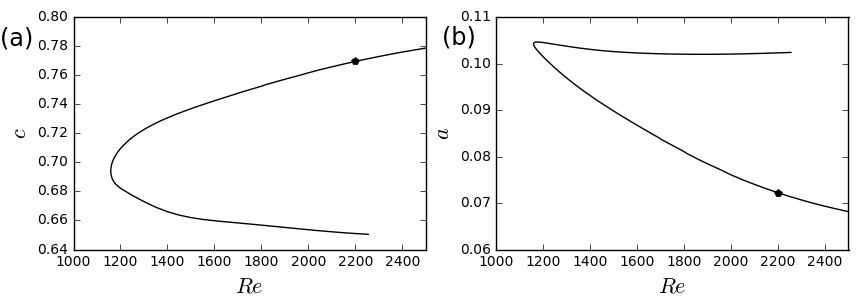
\includegraphics[width=0.9\linewidth]{pipeTW-contin.png}}
\caption{Продолжение решения уравнений Навье-Стокса, имеющего вид бегущей волны, по числу Рейнольдса: (а) зависимость фазовой скорости и (b) амплитуды трехмерной составляющей движения от числа Рейнольдса. Точка соответствует исходному решению, найденному на сепаратрисе.} 
\label{pipeTW_contin_pic}
\end{figure}

Продолжение по числу Рейнольдса решения, имеющего вид бегущей волны, найденного на сепаратрисе, позволило получить новые решения в виде бегущей волны. На рис. \ref{pipeTW_contin_pic} приведены значения фазовой скорости $c_\mathrm{tw}$ и средней по объему трубы амплитуды трехмерной составляющей движения $\V_\mathrm{3D} = \v - \overline{\v}^{x,\theta}$. Как и условно периодические решения, порожденные модельным порывом, решений в виде бегущей волны принадлежат однопараметрическому множеству. Семейство решений, порожденное бегущей волной, найденной на сепаратрисе, возникает в результате бифуркации при $\Re \approx 1200$. При меньших числах Рейнольдса решений из этого семейства не существует. При больших числах Рейнольдса существует две ветви решений. В точке бифуркации производная по числу Рейнольдса от характеристик решения обращается в бесконечность, что не позволяет перейти с одной ветви решения на другую, продлевая решение по числу Рейнольдса. Для того, чтобы перейти с одной ветви решения на другу, вблизи от точки бифуркации продолжение решения было выполнено по фазовой скорости $c_\mathrm{tw}$. Число Рейнольдса, при этом, было включено в число определяемых параметров. Ветвь, которой принадлежит исходное решение, найденное на сепаратрисе, принято называть нижней, так как для нее характерна меньшая интенсивность колебаний (см. рис. \ref{pipeTW_contin_pic}(b)). Решения с верхней ветви по амплитуде колебаний оказываются ближе к турбулентному течения, что делает их привлекательными для исследования. 

\begin{figure}
\center{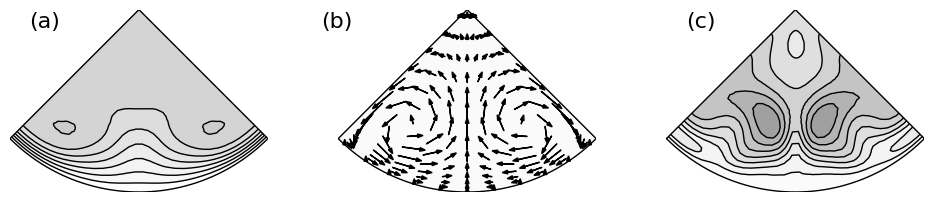
\includegraphics[width=1\linewidth]{pipeTW-1700ub-means.png}}
\center{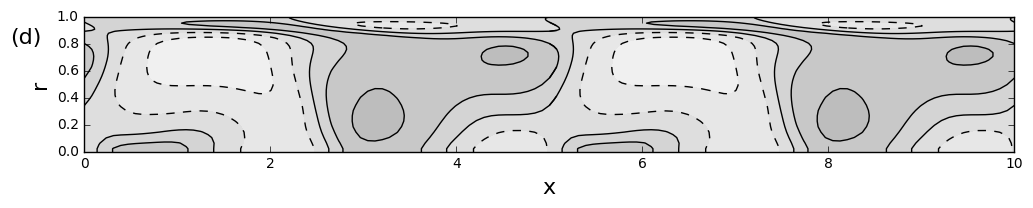
\includegraphics[width=1\linewidth]{pipeTW-1700ub-puls.png}}
\caption{Поле скорости решения, имеющего вид бегущей волны, принадлежащего верней ветви, $\Re = 1700$: (a) --- изолинии средней продольной скорости, (b) --- средняя поперечная скорость, (c) --- линии уровня амплитуды пульсаций, (d) --- изолинии продольной компоненты пульсационной составляющей движения в сечении $\theta = 0$ (продольный период $L_x = 5$). Сплошные линии --- положительные значения, прерывистые -- отрицательным. } 
\label{pipeTWub_means_pic}
\end{figure}

Исходная сетка, на которой были найдены решения, содержит $32 \times 32 \times 32$ ячеек в продольном, радиальном и угловом направлениях. Протяженность расчетной области составляет $L_x = 5R$. Для того, чтобы установить влияние расчетной сетки на результат, решения были пересчитаны на более подробной сетке, содержащей вдвое большее число ячеек в каждом направлении ($64 \times 64 \times 64$). В радиальном направлении введено растяжение сетки таким образом, что высота ячейки вблизи сетки в 4 раза меньше, чем вблизи оси трубы. Таким образом, разрешение сеток, на которых получены решения в виде бегущих волн, точно совпадает с разрешением сток, на которых получен модельный порыв (см. раздел \ref{edge_seq}). Для адекватного воспроизведения решений с верхней ветви требуются более подробные расчетные сетки, чем для решений с нижней ветви. Расчеты, проведенные на двух расчетных сетках, показали, что до $\Re \approx 2000$ решение на верхней ветви воспроизводится адекватно. Также, как при исследовании верхней ветви семейства решений, порожденного модельным порывом, характеристики верхней ветви решений, имеющих вид бегущей волны, будут представлены на примере решения с $\Re = 1700$. Это решение оказывается устойчивым (при наложенных дополнительных условиях симметрии \eqref{sym_eq}, \eqref{per_eq}, \eqref{bc2_eq}). Его фазовая скорость равна $c_\mathrm{tw,ub} = 0.66U$, где $U$ --- удвоенная расходная скорость, совпадающая с максимальной скоростью в течения Пуазейля с аналогичным расходом. 

\begin{figure}
\center{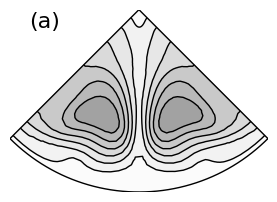
\includegraphics[width=0.33\linewidth]{pipeTW-1700ub-lin-map.png} 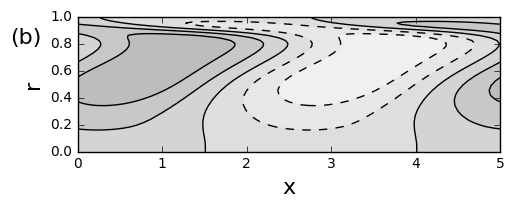
\includegraphics[width=0.6\linewidth]{pipeTW-1700ub-lin-puls.png}}
\caption{Наиболее быстро растущее собственное решение линейной задачи устойчивости поля скорости $\V_\mathrm{tw,ub}$: (a) --- линии уровня амплитуды колебаний; (b) --- изолинии продольной компоненты скорости в сечении $\theta = 0$. Сплошные линии --- положительные значения, прерывистые --- отрицательные.}
\label{pipeTWub_lin_pic}
\end{figure}

Также, как при анализе бегущей волны, найденной на сепаратрисе, выполненном в разделе \ref{pipe_tw_seq}, разделим поле скорости выбранной для анализа бегущей волны $\v_\mathrm{tw,ub}$ на среднюю $\V_\mathrm{tw,ub} = \overline{\v_\mathrm{tw,ub}}^x$ и пульсационную $\v'_\mathrm{tw,ub} = \v_\mathrm{tw,ub} - \V_\mathrm{tw,ub}$ составляющие путем осреднения в продольном направлении $x$, обозначенного чертой над выражением с соответствующим индексом.  Для бегущей волны осреднение в продольном направлении эквивалентно осреднению по времени (при условии, что оно выполнено в системе отсчета, скорость перемещения которой не совпадает с фазовой скоростью волны). Среднее поле скорости зависит только от двух координат, $r$ и $\theta$, что делает его удобным объектом для исследования. 

Также, как и в других исследованных решениях, среднее поле скорости включает полосы повышенной и пониженной скорости, вытянутые вдоль потока. Распределение средней продольной скорости приведено на рис. \eqref{pipeTWub_means_pic}(а). В центральной части трубы, где медленная жидкость проникает ближе к центру трубы, находится полоса пониженной скорости. При большем и меньшем значении $\theta$ находятся полосы повышенной скорости. Отметим, что скорости жидкости в области расположения полос повышенной скорости оказывается даже выше, чем на оси трубы. Существование поло поддерживает слабое движение жидкости в нормальной к основному потоку плоскости. Распределение средней поперечной скорости, приведенное на рис. \ref{pipeTWub_means_pic}(b), соответствует наличию продольных вихрей, поддерживающих существование полос. Там, где медленная жидкость движется от стенки, находятся полосы пониженной скорости. Там, где жидкость движется ближе к стенке --- полосы повышенной скорости. 

\begin{figure}
\center{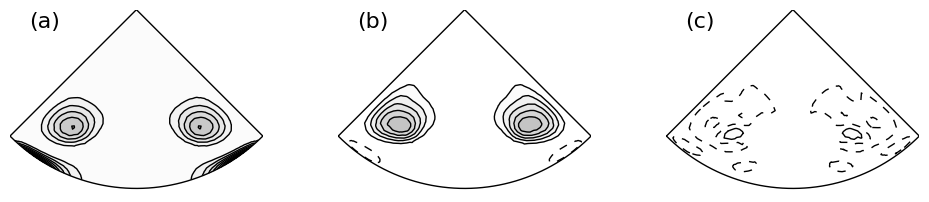
\includegraphics[width=1\linewidth]{pipeTW-1700ub-OXgen.png}}
\caption{Образование продольных вихрей в решении, имеющем вид бегущей волны, принадлежащем верхней ветви, $\Re = 1700$: значение $\Omega_x^2$ (a), вклад в генерацию $\Omega_x^2$ со стороны слагаемых, соответствующих \eqref{OXgen_terms}, (b) и другим слагаемым в правой части \eqref{OX_eq} (с). Сплошные линии --- положительные значения, прерывистые --- отрицательные.}
\label{pipeTWub_OXgen_pic}
\end{figure}

Пульсации оказываются сосредоточены между полосами повышенной и пониженной скорости и, в несколько меньшей степени, в области расположения полос повышенной скорости (см. рис. \ref{pipeTWub_means_pic}(c)). Отметим, что распределения средней скорости и пульсаций в этом случае значительно отличаются от аналогичных распределений для решения с верхней ветви семейства решений, порожденного модельным порывом (см. рис. \ref{local_ub_means_pic}). В решении, порожденном модельным порывом, скорость на оси трубы оказывается выше, чем в полосах повышенной скорости, пульсации достигают максимума между полосами повышенной скорости и осью трубы, интенсивность пульсаций между полосами разных знаков оказывается значительно ниже. По-видимому, это объясняется наличием продольной неоднородность в пространственно-локализованном решении. Мы полагаем, что механизм образования пульсаций в случае рассматриваемой бегущей волны также, как и в других случаях, является линейным. Хотя среднее поле скорости $\V_\mathrm{tw,ub}$ оказывается линейно устойчивым, собственная функция, соответствующая наиболее медленно затухающему собственному решению, $\v'_1$ повторяет форму пульсационной составляющей движения и скорость ее перемещения вдоль трубы. Амплитуда колебаний $\v'_1$ приведена на рис. \ref{pipeTWub_lin_pic}(a). Как и в пульсационной составляющей движения, колебания $\v'_1$ оказываются сосредоточены между полосами повышенной и пониженной скорости, а также, от части, в области расположения полос повышенной скорости. Распределения мгновенной продольной скорости, приведенные для пульсационной составляющей движения $\v'_\mathrm{tw,ub}$ на рис. \ref{pipeTWub_means_pic}(d), а для $\v'_1$ на рис. \ref{pipeTWub_lin_pic}(b), также согласуются друг с другом. Фазовая скорость $\v'_1$ равна $c_1 = 0.63U$, декремент затухания $\lambda_1 = -0.0085U/R$. Линейная устойчивость среднего течения не противоречит тому, что механизм передачи энергии в пульсационную составляющую движения является линейный. Амплитуда колебаний в рассматриваемом решении оказывается достаточно велика и достигает $0.15U$. Полосы повышенной и пониженной скорости в решении смещаются в боковом направлении с достаточно существенной амплитудой, в результате чего среднее течение недостаточно точно воспроизводит форму полос --- угловые градиенты продольной скорости в среднем течении оказываются ниже, чем в неосредненном поле скорости $\v_\mathrm{tw,ub}$, и скорость роста возмущений на среднем поле скорости может оказаться ниже, чем на неосредненном.

\begin{figure}
\center{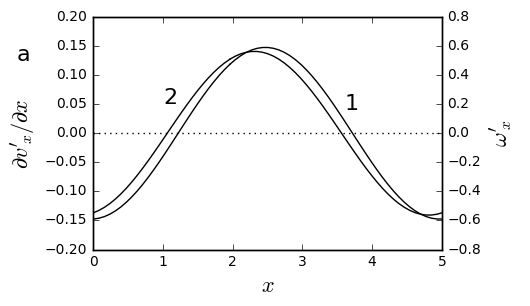
\includegraphics[width=0.5\linewidth]{pipeTW-1700ub-corrA.png}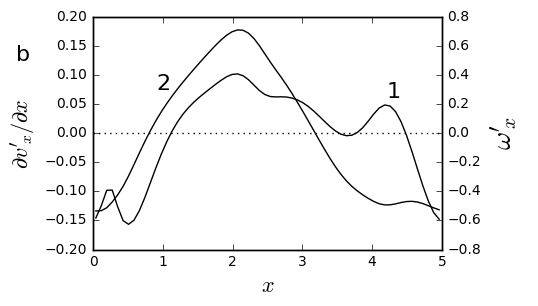
\includegraphics[width=0.5\linewidth]{pipeTW-1700ub-corrB.png}}
\caption{Значения $\d v_x' /\d x$ (кривая 1) и $\omega_x'$ (кривая 2) на прямой, где $\Omega_x$ достигает максимума, $r = 0.75, \theta = \pi/10$: (a) --- для пульсаций, полученных в линейном приближении; (b) --- для пульсационной составляющей движения. }
\label{pipeTWub_corr_pic}
\end{figure}

Существование продольных вихрей, формирующих полосы повышенной и пониженной скорости, объясняется наличием пульсаций. Продольным вихрям, имеющих различные направления вращения, соответствуют области концентрации положительной и отрицательной средней продольной завихренности $\Omega_x$, $(\Omega_x, \Omega_r, \Omega_\theta) = \mathrm{rot} \V_\mathrm{tw,ub}$. Как и в других исследованных решениях, в рассматриваемом решении в уравнении баланса средней продольной завихренности \eqref{OX1_eq} за образование продольных вихрей ответственны слагаемые \eqref{OXgen_terms}, описывающие нелинейное взаимодействие пульсаций продольной скорости и пульсаций продольной завихренности. Работать удобнее с уравнением баланса квадрата средней продольной завихренности $\Omega_x^2$, получаемым умножением уравнения \eqref{OX1_eq} на $2\Omega_x$. Положительное значение источниковых членов в этом уравнении говорит об их положительном вкладе, а отрицательное значение --- об отрицательном. Значение слагаемых \eqref{OXgen_terms}, умноженных на $2\Omega_x$, приведено на рис. \ref{pipeTWub_OXgen_pic}(b). Значение суммы других слагаемых в правой части \eqref{OX1_eq}, умноженных на $2\Omega_x$, приведено на рис. \ref{pipeTWub_OXgen_pic}(c). Слагаемые \eqref{OXgen_terms} определяет форму поля $\Omega_x$ в области расположения продольных вихрей (см. рис. \ref{pipeTWub_OXgen_pic}(a)), другие источниковые слагаемые дают преимущественно отрицательный вклад в подержание продольной завихренности и по амплитуде значительно уступает выделенному слагаемому. Таким образом, нет сомнений, что и в этом случае за образование продольных вихрей отвечают слагаемые \eqref{OXgen_terms}. 

\begin{figure}[h]
\center{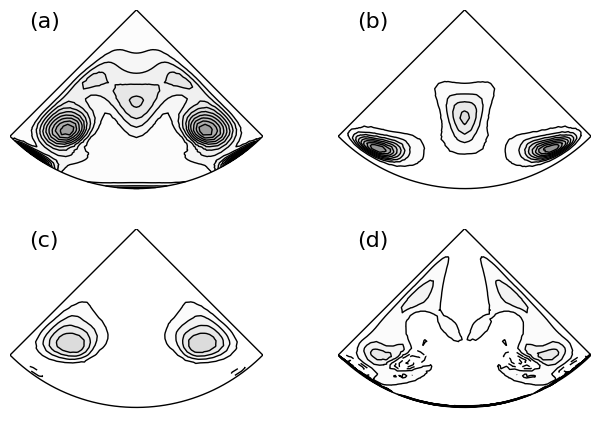
\includegraphics[width=0.66\linewidth]{pipeTW-1700ub-ox1gen.png}}
\caption{Образование пульсаций продольной завихренности в решении, имеющем вид бегущей волны, принадлежащем верхней ветви, $\Re = 1700$: средний квадрат пульсаций продольной завихренности $\overline{\omega'_x \omega'_x }^x$ (а), вклад в производство $\overline{\omega'_x \omega'_x }^x$ слагаемых, соответствующих \eqref{ox1gen_add_terms}, (b), слагаемого, соответствующего \eqref{ox1gen_main_terms}, (c) и слагаемого, соответствующего сумме остальных слагаемых в правой части \eqref{ox2_eq} (d). Сплошные линии --- положительные значения, прерывистые --- отрицательные.}
\label{pipeTWub_ox1gen_pic}
\end{figure}

Пульсации, полученные в рамках линеаризованных уравнений, $\v_1$ также воспроизводят описанный механизм образования продольных вихрей, но имеют более простую форму (их поле скорости меняется вдоль трубы по гармоническому закону), что делает их привлекательным объектом для анализа. Между собой слагаемые \eqref{OXgen_terms} оказываются равны в силу периодичности поля скорости вдоль потока, поэтому мы ограничимся анализом второго из слагаемых. Отличие от нуля этого слагаемого говорит о наличие корреляции между пульсациями продольной скорости и пульсациями продольной завихренности, причем эта корреляция такова, что в области расположения положительного вихря $\omega'_x$ и ${\partial v'_x}/{\partial x}$ имеют положительную корреляцию, а в области расположения отрицательного вихря --- отрицательную, что позволяет поддерживать существование этих вихрей. Для того, чтобы продемонстрировать наличие корреляции, на рис. \ref{pipeTWub_corr_pic} приведено значение $\omega'_x$ и ${\partial v'_x}/{\partial x}$ на прямой, параллельной оси $x$, проходящей через центр положительного вихря ($\Omega_x$ достигает максимума), $r = 0.75, \theta = \pi/10$. На рисунке (a) приведены значения для пульсаций, полученных в рамках линеаризованных уравнений, $\v'_1$. Кривые меняются вдоль потока по гармоническому закону и оказываются в фазе друг с другом, что обеспечивает наибольшую эффективность производства $\Omega_x$. На рисунке (b) приведены аналогичные значения для пульсационной составляющей движения $\v'_\mathrm{tw,ub}$. Хотя графики имеют значительно более сложную форму, чем в линейном случае или в случае аналогичного решения с нижней ветви (см. рис. \ref{OXgen_corr_pic}), они также согласованы друг с другом (кривые достигают наибольшего и наименьшего значения в близких точках). Наличие корреляции объясняется механизмом образования пульсаций продольной завихренности $\omega'_x$, согласующемся в рассматриваемом решении и в других исследованных решениях (см. раздел \ref{ox1gen_seq}). 

В уравнении \eqref{ox2_eq} за образование пульсаций продольной завихренности $\omega'_x$ в области расположения продольных вихрей ответственно слагаемое \eqref{ox1gen_main_terms}, отписывающее эффект сжатия и растяжения существующих в потоке вихревых трубок, вызванного пульсациями продольной скорости. Для того, чтобы продемонстрировать вклад слагаемого \eqref{ox1gen_main_terms} в образование $\omega'_x$, обратимся к уравнению баланса среднего квадрата пульсаций продольной завихренности $\overline{\omega'_x\omega'_x}^x$, полученного умножением \eqref{ox2_eq} на $2\omega'_x$ с последующим определением по $x$. Слагаемые в этом уравнении зависят только от $r$ и $\theta$, положительное значение источниковых членов в этом уравнении говорит об их содействии образованию $\omega'_x$, а отрицательное --- о противодействии. На рис. \ref{pipeTWub_ox1gen_pic} приведено значение $\overline{\omega'_x\omega'_x}$ (a) и вклада в его образование со стороны слагаемых, соответствующих \eqref{ox1gen_add_terms}, (b), слагаемого, соответствующего \eqref{ox1gen_main_terms}, (c) и слагаемых, соответствующих сумме других слагаемых в правой части уравнения \eqref{ox2_eq}. Наибольший вклад в образование $\omega'_x$ дают слагаемые \eqref{ox1gen_add_terms}, отвечающие за поворот нормальных к стенке вихревых нитей на фоне нормального к стенке градиента скорости. Хотя эти слагаемые имеют существенное значение вблизи области расположения продольных вихрей, они не участвуют в поддержании продольных вихрей, так как пульсации, формируемые этими слагаемыми, согласованы с пульсациями продольной скорости таким образом, что их нелинейное взаимодействие отсутствует (см. раздел \ref{ox1gen_seq}). Образование пульсаций $\omega'_x$ в области расположения продольных вихрей связано со слагаемым \eqref{ox1gen_main_terms}. Именно это слагаемое обеспечивает необходимую для поддержания продольных вихрей согласованность между пульсациями продольной скорости и пульсациями продольной завихренности. Другие источниковые слагаемые в области расположения продольных вихрей имеют как положительное, так и отрицательное значение, и существенного влияния на образование $\omega'_x$ в интересующей нас области не оказывают. 

Таким образом, для рассмотренного решения, имеющего вид бегущей волны, принадлежащего верхней ветви, механизм образования колебаний оказывается таким же, как и для других исследованных решений за тем исключением, что среднее поле скорости оказывается линейно устойчивым. Тем не менее, эта особенность решения не говорит о том, что механизм передачи энергии в пульсационную составляющую движения отличается от линейного. 



\begin{comment}
Re2200ub:
lin: cf = 0.44473618074359494, lambda = -0.0085
vwz: cf = 0.6470799307435949, lambda = -0.021

Re1700ub:
lin: cf = 0.633021694959945, lambda = -0.02
vwz: cf = 0.651179838899339, lambda = -0.028 (unsym)
        Осесимметричное возмущение, lambda = -0.028
\end{comment}

\section{Семейство решений уравнений Навье-Стокса в виде бегущих волн в плоском течении Пуазейля}

Кроме движения жидкости в круглой трубе в работе также было исследованы некоторые случаи движения жидкости в плоском канале Пуазейля. Постановка задачи в этом случае близка к постановке в круглой трубе. В области течения вводится ортогональная системы координат $(x,y,z)$. Ось $x$ направлена вдоль потока, ось $y$ --- по нормали к стенке, ось $z$ --- в трансверсальном направлении. Движение жидкости полагается удовлетворяющем уравнениям Навье-Стокса \eqref{NSeq_Re} и условию несжимаемости \eqref{eq0_Re}. На твердой стенке, расположенной при $y = 0$, ставятся условия прилипания:
\begin{equation}
\v = 0 \text{, при } y = 0
\end{equation}
При $y = 1$ ставится условие проскальзывания, аналогичное условию на оси трубы при дополнительных условиях симметрии в угловом направлении \eqref{sym_eq} и \eqref{per_eq}. Условие проскальзывания имеет вид:
\begin{equation}
\pd{u}{y} = v = \pd{w}{y} = \pd{p}{y} = 0 \text{, при } y = 1
\end{equation}
Здесь $(u,v,w)$ --- компоненты вектора скорости в декартовой системе координат. В качестве единицы длины, таким образом, выступает полуширина канала. Вдоль потока и в трансверсальном направлении ставятся условия периодичности с периодом $L_x$ и $L_z$ соответственно:
\begin{equation}\label{duct_xper_eq}
(\v,p)(x,y,z) = (\v,p)(x+L_x,y,z)
\end{equation}
\begin{equation}\label{duct_zper_eq}
(\v,p)(x,y,z) = (\v,p)(x,y,z+L_z)
\end{equation}
Также, по аналогии с постановкой задачи в трубе, в трансверсальном направлении ставится условие отражения относительно плоскости $z = 0$:
\begin{equation}\label{duct_sym_eq}
(u,v,w,p)(x,y,z) = (u,v,-w,p)(x,y,-z)
\end{equation}
Условия \eqref{duct_zper_eq} и \eqref{duct_sym_eq} могут быть заменены условиями проскальзывания при $z = 0$ и $z = L_z/2$, имеющим вид:
\begin{equation}
\pd{u}{z} = \pd{v}{z} = w = \pd{p}{z} = 0 \text{, при } z = 0, L_z/2 
\end{equation}
Таким образом, расчетная область представляет собой параллелепипед размера $L_x \times 1 \times L_z/2$. Жидкость приводится в движение внешним перепадом давления, определяемым из условия постоянства удельного расхода. В качестве единицы скорости выступает наибольшая скорость в течении Пуазейля. Условие постоянства удельного расхода в безразмерном виде имеет в этом случае вид:
\begin{equation}
\frac{1}{S}\int_{S} u\,dy\,dz = 2/3
\end{equation}
Здесь $S$ --- поперечное сечение трубы и его площадь. Задача поставлена. 


\begin{figure}
\center{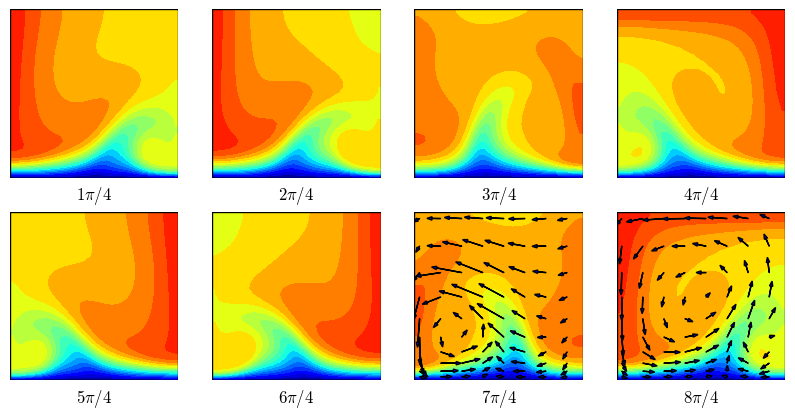
\includegraphics[width=1\linewidth]{duct_turb_map.png}}
\caption{Поле скорости бегущей волны, выделенной из турбулентного течения в плоском канале. Приведена продольная скорости в поперечном сечении в различные фазы течения. На последних двух изображениях приведена также поперечная компонента движения. Твердая стенка находится внизу.} 
\label{duct_turb_tw_pic}
\end{figure}

Было обнаружено, что в расчетной области небольшого размера при небольших значениях числа Рейнольдса турбулентное движение напоминает некоторую бегущую волну. Турбулентное поле скорости оказалось удачным начальным приближением для точной бегущей волны, с которым метод Ньютона сходится. Бегущую волну можно рассматривать, как частный случай условно периодического по времени решения. Для её нахождения может быть использован код, написанный для поиска периодических решений. Параметр $T$, выступающий в качестве периода решения по времени, в данном случае выступает в качестве параметра расчета, не влияющего на результат. Однако отметим, что увеличения значения $T$ позволяет существенным образом сократить число итераций метода решения линейной системы, выполняемого на каждом шаге метода Ньютона. 


\begin{figure}
\center{\includegraphics[width=0.45\linewidth]{duct_turb_tw_cf.png}\includegraphics[width=0.45\linewidth]{duct_turb_tw_umean.png}}
\caption{(a) --- зависимость фазовой скорости волны $c$ от числа Рейнольдса $\Re$, черной точкой обозначено исходное решение, принадлежащее верхней ветви; (b) --- средний профиль скорости решения типа бегущей волны с нижней и верхней ветвей, $\Re = 1400$.} 
\label{duct_turb_tw_contin}
\end{figure}


Бегущая волна из турбулентного течения выделена при $L_x = 5$, $L_z = 2$, $\Re = 1400$. Её фазовая скорости равна $c_{tw} = 0.73$. Расчетная сетка, на которой было найдено решение, содержит $64 \times 40 \times 32$ ячеек. Форму бегущей волны позволяет представить рисунок \ref{duct_turb_tw_pic}. На нем изображена продольная скорость в нескольких сечениях трубы, покрывающих один период изменения решения в пространстве (а также во времени). В центре расчетной области около стенки можно выделить полосу замедления, смещающуюся периодическим образом в направлении $z$. Она возникает за счет действия вихрей, расположенных по бокам от полосы замедления в шахматном порядке. Для того, чтобы продемонстрировать существование вихрей, на рисунке \ref{duct_turb_tw_pic} в двух сечения представлена также поперечная компонента скорости. Хотя основные элементы цикла самоподдержания в бегущей волне присутствуют, повторить рассуждения, разработанные при исследовании модельного порыва, для этого решения в полной мере не удается. Амплитуда смещения полосы замедления оказывается слишком велика, так что стандартный метод разделения поля скорости на среднюю и пульсационную составляющие не дает ожидаемого результата. Среднее течение, полученное таким образом, не адекватно воспроизводит форму полос. Метод продления решения по параметру позволяет перевести выделенную бегущую волну к тем значениям параметров, при которых стандартный метод разделения на среднюю и пульсационную составляющие движения дает ожидаемый результат. 




Продлевая выделенную бегущую волну в сторону снижения числа Рейнольдса, удалось достичь точки бифуркации при $\Re = 630$, в которой рождается две ветви решения, и перейти с верхней ветви решения на нижнюю. Зависимость фазовой скорости волны $c_{tw}$ от числа Рейнольдса $\Re$ приведена на рисунке \ref{duct_turb_tw_contin}(a). Для нижней ветви характерны меньшая амплитуда пульсаций, большая фазовая скорость, однако структура решения сохраняется. На рисунке \ref{duct_turb_tw_contin}(b) приведен средний профиль скорости для исходного решения и решения с нижней ветви при том же числе Рейнольдса $\Re = 1400$. Профиль скорости наполненный, на нижней и верхней ветви отличается мало и напоминает профиль скорости в турбулентном потоке. Для дальнейшего анализа выбрано решение, для которого также $\Re = 1400$, $c_{tw} = 0.8$. 

\begin{figure}
\center{\includegraphics[width=0.9\linewidth]{duct_turb_low_tw_map.png}}
\caption{Нижняя ветвь решения типа бегущей волны, $\Re = 1400$. Приведены: (a) --- средняя продольная компонента скорости $U$, (b) --- средняя поперечная компонента скорости $(V,W)$, (c) --- амплитуда пульсаций $\v_n$.} 
\label{duct_turb_tw_pic}
\end{figure}

Поле скорости $\v$ решения с нижней ветви разделяется на среднюю $\V = \overline{\v}^x$ и пульсационную $\v_n = \v - \V$ составляющие осреднением вдоль трубы. В этом случае среднее поле скорости воспроизводит полосы пониженной и повышенной скорости. Продольная компонента среднего поля скорости $U$ изображена на рисунке \ref{duct_turb_tw_pic}(a). Полоса замедления проходит через центр расчетной области вблизи стенки. Полосы ускорения расположены на границах расчетной области при $z = 0$ и $z = 1$. Полосы возникают с результате действия продольных вихрей. На рисунке \ref{duct_turb_tw_pic}(b) представлена поперечная компонента скорости среднего течения $(V,W)$. Поперечное движение может быть ассоциировано с парой продольных вихрей, расположенных по бокам от полосы замедления. Пульсационная составляющая движения возникает в результате периодического смещения полосы замедления в угловом направлении. Амплитуда пульсаций приведена на рисунке \ref{duct_turb_tw_pic}(c). Они сосредоточены в областях между полосами пониженной и повышенной скорости. Как и в других случаях, пульсационная составляющая движения в этом случае возникает в результате линейной неустойчивости среднего течения. Можно отметить, что и в этом случае поле скорости $(U,0,0)$ оказывается линейно устойчиво, так что пренебрежение поперечным движением качественно меняет характеристики устойчивости среднего течения. 

\begin{figure}
\center{\includegraphics[width=0.9\linewidth]{duct_turb_tw_OXgen.png}}
\caption{Механизм генерации $\Omega_x$ для бегущей волны в плоском канале. Приведено значение $\Omega_x^2$ (a) и вклад в его образование со стороны слагаемых \eqref{OXgen_terms} (b) и суммы других слагаемых в правой части уравнения \eqref{OX_eq} (c).} 
\label{duct_turb_tw_OXgen_pic}
\end{figure}

Выделенное решение позволяет наиболее ярко продемонстрировать механизм образования продольной завихренности. Продольным вихрям соответствуют области повышенной амплитуды стационарной продольной завихренности $\Omega_x$. Квадрат стационарной продольной завихренности изображен на рисунке \ref{duct_turb_tw_OXgen_pic}(a). Форму поля продольной завихренности определяет слагаемое \eqref{OXgen_terms}. Его вклад в $\Omega_x^2$ приведен на рисунке \ref{duct_turb_tw_OXgen_pic}(b). Вклад других слагаемых в правой части уравнения \eqref{OX_eq} представлен на рисунке \ref{duct_turb_tw_OXgen_pic}(с). Их суммарное влияние незначительно, хотя оказывается положительным. Таким образом, нет сомнения, что за образование продольных вихрей ответственны слагаемые \eqref{OXgen_terms}, как и в предыдущих случаях. 

\begin{figure}
\center{\includegraphics[width=1\linewidth]{duct_turb_tw_ox1gen.png}}
\caption{Механизм генерации $\omega_x'$ для бегущей волны в плоском канале. Приведено значение $\overline{\omega'_x \omega'_x}^x$ (a) и вклад в его образование со стороны слагаемых \eqref{ox1gen_add_terms} (b), \eqref{ox1gen_main_terms} (c) и других слагаемых в правой части уравнения \eqref{ox1_eq} (d).}
\label{duct_turb_tw_ox1gen_pic}
\end{figure}

Образование пульсаций продольной завихренности $\omega'_x$ также происходит в соответствии с выделенным в работе механизмом. Средний вдоль трубы квадрат $\omega'_x$ приведен на рисунке \ref{duct_turb_tw_ox1gen_pic}(a). Как и в предыдущих случаях, на месте продольных вихрей определяющий вклад дает слагаемое \eqref{ox1gen_main_terms}. Его вклад в $\overline{\omega'_x \omega'_x}$ изображен на рисунке  \ref{duct_turb_tw_ox1gen_pic}(c). На рисунке \ref{duct_turb_tw_ox1gen_pic}(b) приведен вклад слагаемого \eqref{ox1gen_add_terms}, связанного с наклоном нормальных к стенке вихрей, возникающих в пульсационной составляющей движения. В отличии от случае модельного порыва, в этом случае на месте продольных вихрей вклад этого слагаемого пренебрежимо мал, что гарантирует, что оно не участвует в образовании продольных вихрей. Вклад других слагаемых, приведенных на рисунке \ref{duct_turb_tw_ox1gen_pic}(с) оказыватеся отрицательным на месте продольных вихрей. Это вновь может говорить о неточности при разделении слагаемых уравнения \eqref{ox1_eq} на связанные и несвязанные с образование продольной завихренности группы.



В плоском канале может быть найдено решение на сепаратрисе. Метод поиска решения на сепаратрисе в непротяженной расчетной области в постановке, приведенной в предыдущем разделе, позволяет получить бегущую волну, представляющую еще одно семейство решений. Расчеты были выполнены при $L_x = 5$, $L_z = 2.4$, $\Re = 2000$. Возникающая на сепаратрисе бегущая волна в этом случае имеет фазовую скорость $c_{tw} = 0.97$, что близко к максимальной скорости в потоке. Средний профиль её скорости мало отличается от профиля ламинарного течения. Интенсивность пульсаций и движения в поперечной плоскости в этом случае на порядок ниже, чем в бегущей волне, выделенной из турбулентного течения. Тем не менее, структура течения оказывается такой же, как и в других исследованных течениях. В потоке может быть выделена полоса замедления, проходящая через центра расчетной области. Продольная компонента среднего поля скорости $U$ приведена на рисунке \ref{duct_edge_tw_means_pic}(a). В этом случае полоса замедления, как и другие особенности решения, оказывается значительно удалена от твердой стенки. За образование полосы замедления ответственно вторичное течение. Поперечная компонента среднего течения приведена на рисунке \ref{duct_edge_tw_means_pic}(b). Она соответствует паре продольных вихрей, расположенных по бокам от полосы замедления, поддерживающих её существование. Пульсационная составляющая движения сосредоточена в центре канала, и соответствует периодическому смещению области замедления в направлении $z$. Амплитуда пульсаций представлена на рисунке \ref{duct_edge_tw_means_pic}(с). Как и в предыдущих случаях, пульсационная составляющая движения возникает вследствие линейной неустойчивости среднего течения. Кроме того, учет поперечных компонент среднего течения при исследовании его на устойчивость необходим, так как поле скорости $(U,0,0)$ линейной устойчиво. 


\begin{figure}
\center{\includegraphics[width=0.9\linewidth]{duct_edge_tw_means.png}}
\caption{Бегущая волна, возникающая на сепаратрисе в плоском канале, $\Re = 2000$. Приведена стационарная продольная составляющая скорости $U$ (a), стационарная поперечная составляющая скорости $(V,W)$ (b) и амплитуда пульсаций $\v_n$ (с).} 
\label{duct_edge_tw_means_pic}
\end{figure}

Механизм образования продольных вихрей в этом случае также согласуется с уже существующими представлениями. Продольные вихри соответствуют областям повышенной концентрации продольной завихренности $\Omega_x$. Квадрат стационарной продольной завихренности $\Omega_x^2$ изображен на рисунке \ref{duct_edge_tw_OXgen_pic}(a). Нет сомнений, что за образование стационарных продольных вихрей ответственны слагаемые \eqref{OXgen_terms}. Их вклад в формирование $\Omega_x^2$ представлен на рисунке \ref{duct_edge_tw_OXgen_pic}(b). Он значительно превосходит по величине вклад других слагаемых, приведенный на рисунке \ref{duct_edge_tw_OXgen_pic}(c), и определяет форму поля $\Omega_x^2$. Механизм образования пульсаций продольной завихренности $\omega'_x$ в этом случае также согласуется с уже разобранными случаями. 

\begin{figure}
\center{\includegraphics[width=0.9\linewidth]{duct_edge_tw_OXgen.png}}
\caption{Механизм генерации продольных вихрей в бегущей волне, возникающей на сепаратрисе. Приведено значение $\Omega_x^2$ (a) и вклада в его образование со стороны слагаемых \eqref{OXgen_terms} (b) и суммы других слагаемых в правой части уравнения \eqref{OX_eq} (c).}
\label{duct_edge_tw_OXgen_pic}
\end{figure}


\section{Выводы по главе}

В работе, кроме модельного порыва, были найдены и другие инвариантные решения, также допускающие строгое исследование. Их анализ в некоторой степени позволяет установить общность полученных при исследовании модельного порыва результатов. Для всех исследованных решений основные элементы цикла самоподдержания сохраняются, что говорит об их универсальности и позволяет надеяться, что в некотором виде они могут быть найдены в пристенном турбулентном течении непосредственно. 

Продлевая модельный порыв по числу Рейнольдса удалось получить новое условно периодическое локализованное в пространстве решение. Его характеристики оказываются ближе к характеристикам турбулентного порыва, и мы полагаем, что полученные при его исследовании результаты имеют большее отношение к турбулентности. Его анализ показал, что все особенности движения, выделенные при изучении модельного порыва, в полной мере справедливы для найденного решения. Так как оба решения являются представителями одного семейства, можно ожидать, что они воспроизводят общий физический механизм самоподдержания. Тем не менее, полученный результат говорит о том, что механизм самоподдержания сформулирован нами в подходящих терминах; выделенные особенности движения связаны с механизмом самоподдержания существенным образом. 

Также, в плоском канале удалось выделить бегущую волну непосредственно из турбулентного течения. Можно ожидать, что найденное решение воспроизводит особенности, характерные для пристенной турбулентности, хотя её динамика была значительным образом редуцирована наложением условий периодичности в продольном и трансверсальном направлениях. Это может привести к формированию в течении структур, не характерных для свободного турбулентного течения. Важно, что кроме дополнительных условий периодичности, других условий, навязывающих структуру течению, нет. В потоке естественным образом формируется полоса пониженной скорости, расположенная вблизи стенки трубы. Она подвержена значительным по амплитуде колебаниям, что не позволяет, применяя стандартный метод, разделить поле скорости на среднюю и пульсационную части. Однако выделенное решение продлением по числу Рейнольдса было приведено к параметрам, при которых амплитуда пульсаций снижается до уровня, при котором стандартный метод разделения дает желаемый результат. Для полученного таким образом решения справедливы все особенности движения, связанные с числом самоподдержания, выделенные в работе.

Также в плоском канале было была получена бегущая волна, принадлежащая сепаратрисе. Для неё характерна низкая амплитуда вторичного течения и пульсаций, её среднее поле скорости существенно отличается от поля скорости бегущей волны, выделенной в турбулентном течении, однако и в этом решении основные особенности движения, связанные с циклом самоподдержания, выделены. Кроме представленных в главе решений, в работе были получены некоторые другие инвариантные решения. В частности, удалось выделить бегущую волну из турбулентного течения в круглой трубы. Оказалось, что выделенная бегущая волна принадлежит тому же семейству, которому принадлежит бегущая волна, возникающая на сепаратрисе, но если вторя принадлежит нижней ветви, то первая -- верхней. Бегущая волна с верхней ветви повторяет форму бегущей волны, возникающую внутри модельного порыва на верхней ветви. В силу свой избыточности, результаты для неё в главе не приведены. 

Можно отметить, что в ряде случаев есть основания полагать, что слагаемые, отвечающие за формирование продольных вихрей, выделены не точно. Вероятно, уточнить их позволит развитие представлений о физическом механизме, ответственном за этот процесс. Кроме того, метод разделения на среднюю и пульсационную составляющие течения оказался не эффективным при исследовании бегущей волны, выделенной из турбулентного течения. Вероятно, аналогичные сложности могут возникнуть при изучении турбулентного течения непосредственно. Для преодоления возникшего затруднения необходимо разработать новый метод разделения течения на компоненты, пригодный для потоков с большой амплитудой пульсаций.

То обстоятельство, что выделенный при изучении течения в трубе механизм самоподдержания справедлив также и для течений в плоском канале говорит о том, что он связан с кривизной стенки существенным образом. 

Отметим также, что все исследованные решения найдены при условии отражения в трансверсальном направлении. Существует вероятность, что такое условие навязывает некоторую структур течению, не характерную для свободных потоках. 







\addcontentsline{toc}{chapter}{Заключение}
\chapter*{Заключение} 

%В заключении диссертации излагаются 1) итоги выполненного исследования, 2) выводы, 3) рекомендации, 4) перспективы дальнейшей разработки темы.

В геометрии течения в круглой трубе рассчитан модельный порыв --- условно периодическое решение уравнений Навье-Стокса с пространственно-локализованной структурой, являющееся предельным состоянием решения, эволюционирующего на сепаратрисе, разделяющей в фазовом пространстве области притяжения решений, соответствующих ламинарному и турбулентному режимам течения. Описана внутренняя структура модельного порыва и его основные характеристики. Показано, что модельный порыв воспроизводит ряд качественных особенностей турбулентных порывов, наблюдаемых в круглых трубах при переходных числах Рейнольдса. Также, как в турбулентном порыве, в модельном порыве можно выделить вытянутые вдоль потока полосы повышенной и пониженной скорости, но если в первом случае эти полосы перемещаются вдоль стенки и их сплошность разрываются флуктуирующей составляющей движения, то во втором случае они сохраняют свое положение в пространстве и подвержены лишь небольшим колебаниям. Простое временное поведение модельного порыва позволило выполнить его детальное исследование. Полученные при исследовании модельного порыва результаты, мы полагаем, будут полезны для понимания турбулентного порыва. 

Установить универсальность наблюдаемых в модельном порыве закономерностей движения позволяет анализ других инвариантных решений Навье-Стокса, рассчитанных в работе. Методом продолжения по параметру рассчитано соответствующее модельному порыву семейство условно периодических решений уравнений Навье-Стокса с пространственно-локализованной структурой. В частности, найдены решения, оказывающиеся по ряду качественных характеристик ближе к турбулентному порыву, чем модельный порыв. Можно ожидать, что выводы, сделанные на основе исследования модельного порыва и этих решений имеют большее отношение к турбулентному порыву, чем выводы, сделанные при исследовании только модельного порыва. Также в геометрии течения в круглой трубе и течения в плоском канале найдено три семейства решений, имеющих вид бегущей волны. Анализ всех найденных решений позволяет сформулировать идеализированный цикл поддержания колебаний в такого рода решениях. 

Поле скорости каждого решения может быть представлено в виде суммы средней и пульсационной составляющих. Во всех исследованных решениях в среднем течении существуют вытянутые вдоль потока полосы повышенной и пониженной скорости, чередующиеся в угловом (поперечном) направлении. В случае решения в виде бегущей волны среднее поле скорости не зависит от продольной координаты и, соответственно, полосы имеют неограниченную протяженность. В случае решений с пространственно-локализованной структурой полосы имеют ограниченную протяженность. Возбуждение пульсаций связано с линейной неустойчивостью среднего течения. Колебания оказываются сконцентрированы в промежуточных областях между соседними полосами повышенной и пониженной скорости. В этих областях распределение среднее продольной скорости имеет точки перегиба, если рассматривать его как функцию угловой (поперечной) координаты, что позволяет связать неустойчивость среднего течения с неустойчивость струйных течений с точками перегиба. За поддержание полос ответственны продольные вихри, перемещающие жидкость в нормальной к основному потоку плоскости. 

Существенным результатом работы является описание нелинейного механизма поддержания продольных вихрей. Показано, что во всех решениях продольные вихри образуются в результате нелинейного взаимодействия пульсаций продольной скорости и пульсаций продольной завихренности. Пульсации продольной завихренности в области расположения продольных вихрей образуются за счет сжатия и растяжения существующих вихревых трубок пульсациями продольной скорости, что обеспечивает необходимую для поддержания продольных вихрей согласованность фаз между этими пульсациями. Отметим, что продольные вихри образуются в областях возникновения пульсаций, между полосами повышенной и пониженной скорости, так как именно в этих областях пульсации имеют наибольшую амплитуду и средняя скорость жидкость совпадает с фазовой скоростью пульсаций, что необходимо для образования пульсаций продольной завихренности описанным механизмом. Таким образом, продольные вихри образуются в промежуточной области между полосами повышенной и пониженной скорости, оказываясь расположенными наиболее удачным образом для поддержания существования этих полос. 

Наиболее быстрорастущее решение линейной задачи устойчивости среднего течения также воспроизводит описанный механизм поддержания продольных вихрей, но только в том случае, если при анализе среднего течения на устойчивость учтена не только продольная но и поперечная компоненты средней скорости. Принято считать, что поперечная компонента движения, поддерживая угловую (поперечную) неоднородность среднего течения, не оказывает существенного влияния на характеристики устойчивости среднего течения. Мы видим, что учет поперечной компоненты среднего течения необходим для адекватного воспроизведения механизма поддержания колебаний. 

Полосчатые структуры являются неотъемлемым элементом всех сценариев самоподдержания турбулентности в пристенных течениях, что говорит о вероятной близости выделенного в работе механизма с механизмом самоподдержания однородной (нелокализованной) пристенной турбулентности. На следующем этапе выполнения работы необходимо установить применимость сделанных выводов к турбулентному порву, и к более широкому классу пристенных турбулентных течений. Для этого, по-видимому, необходимо разработать метод промежуточного осреднения, позволяющий выделить в реальном турбулентном течении крупномасштабные и мелкомасштабные структуры. Это позволит обобщить рассуждения, применяемые в работе, на такого рода течения. Имея представления о механизме поддержания колебаний можно предложить эффективные стратегии управления турбулентными течениями с целью снижения или увеличения интенсивности колебаний. Эти стратегии также могут быть опробованы на реальных пристенных турбулентных течениях (численно), и в зависимости от их эффективности могут быть сделаны выводы о роли выделенных механизмов в поддержании такого рода режимов течения. В случае, если разработанные стратегии управления турбулентными потоками покажут себя эффективными, они имеют собственную значительную ценность. 







\newcommand{\listpub}{Список литературы}
\renewcommand{\bibname}{\listpub}

\phantomsection
\addcontentsline{toc}{chapter}{\tocsecindent{\listpub}}
\bibliography{bib/base,bib/rus,bib/books,bib/my}


\end{document}
